% ---------------------------------------------------------------------------------------------------------------
% TEMPLATE PARA TRABALHO DE CONCLUSÃO DE CURSO
% Universidade Federal do Sul e Sudeste do Pará - UNIFESSPA
% Customização da classe abnTeX2 (http://www.abntex.net.br/) para as normas da UTFPR
%
% Projeto hospedado em: <link git>
% Autores: Warley Junior
%
%----------------------------------------------------------------------------------------------------------------
% Codificação: UTF-8
% LaTeX:  abnTeX2          
% ---------------------------------------------------------------------------------------------------------------


% CARREGA CLASSE PERSONALIZADA DA UNIFESSPA--------------------------------------------------------------------------
\documentclass[%twoside,                   % Impressão em frente e verso
    	        oneside,                   % Impressão apenas frente
]{configuracoes/utfpr-abntex2}


% INCLUI ARQUIVOS DE CONFIGURAÇÕES-------------------------------------------------------------------------------
% REFERÊNCIAS------------------------------------------------------------------
\usepackage[%
    alf,
    abnt-emphasize=bf,
    bibjustif,
    recuo=0cm,
    abnt-url-package=url,       % Utiliza o pacote url
    abnt-refinfo=yes,           % Utiliza o estilo bibliográfico abnt-refinfo
    abnt-etal-cite=3,
    abnt-etal-list=3,
    abnt-thesis-year=final
]{abntex2cite}                  % Configura as citações bibliográficas conforme a norma ABNT

% PACOTES----------------------------------------------------------------------
\usepackage[utf8]{inputenc}                                 % Codificação do documento
\usepackage[T1]{fontenc}                                    % Seleção de código de fonte
\usepackage{booktabs}                                       % Réguas horizontais em tabelas
\usepackage{color, colortbl}                                % Controle das cores
\usepackage{float}                                          % Necessário para tabelas/figuras em ambiente multi-colunas
\usepackage{array,multirow,graphicx}                                       % Inclusão de gráficos e figuras
\usepackage{icomma}                                         % Uso de vírgulas em expressões matemáticas
\usepackage{indentfirst}                                    % Indenta o primeiro parágrafo de cada seção
\usepackage{microtype}                                      % Melhora a justificação do documento
\usepackage{multirow, array}                                % Permite tabelas com múltiplas linhas e colunas
\usepackage{subeqnarray}                                    % Permite subnumeração de equações
\usepackage{lastpage}                                       % Para encontrar última página do documento
\usepackage{verbatim}                                       % Permite apresentar texto tal como escrito no documento, ainda que sejam comandos Latex
\usepackage{amsfonts, amssymb, amsmath}                     % Fontes e símbolos matemáticos
\usepackage[algoruled, portuguese]{algorithm2e}             % Permite escrever algoritmos em português
%\usepackage[scaled]{helvet}                                % Usa a fonte Helvetica
\usepackage{times}                                          % Usa a fonte Times
%\usepackage{palatino}                                      % Usa a fonte Palatino
%\usepackage{lmodern}                                       % Usa a fonte Latin Modern
\usepackage[bottom]{footmisc}                               % Mantém as notas de rodapé sempre na mesma posição
\usepackage{ae, aecompl}                                    % Fontes de alta qualidade
\usepackage{latexsym}                                       % Símbolos matemáticos
\usepackage{lscape}                                         % Permite páginas em modo "paisagem"
%\usepackage{picinpar}                                      % Dispor imagens em parágrafos
%\usepackage{scalefnt}                                      % Permite redimensionar tamanho da fonte
%\usepackage{subfig}                                        % Posicionamento de figuras
%\usepackage{upgreek}                                       % Fonte letras gregas

% Redefine a fonte para uma fonte similar a Arial (fonte Helvetica)
%\renewcommand*\familydefault{\sfdefault}

\usepackage{float}

\usepackage{subfig}

\usepackage{array}
\newcolumntype{C}[1]{>{\centering\arraybackslash}p{#1}}

% marcadores especiais para a as tabelas
\usepackage{pifont}
\newcommand{\xmark}{\ding{55}}
\newcommand{\cmark}{\ding{51}}

\usepackage{enumitem}

\usepackage{tabularx}
\usepackage{svg}

\usepackage{pdfpages}

% CONFIGURAÇÕES DE APARÊNCIA DO PDF FINAL--------------------------------------
\makeatletter
\hypersetup{%
    portuguese,
    colorlinks=false,   % true: "links" coloridos; false: "links" em caixas de texto
    linkcolor=blue,    % Define cor dos "links" internos
    citecolor=blue,    % Define cor dos "links" para as referências bibliográficas
    filecolor=blue,    % Define cor dos "links" para arquivos
    urlcolor=blue,     % Define a cor dos "hiperlinks"
    breaklinks=true,
    pdftitle={\@title},
    pdfauthor={\@author},
    pdfkeywords={abnt, latex, abntex, abntex2}
}
\makeatother

% ALTERA O ASPECTO DA COR AZUL--------------------------------------------------
\definecolor{blue}{RGB}{41,5,195}

% REDEFINIÇÃO DE LABELS---------------------------------------------------------
\renewcommand{\algorithmautorefname}{Algoritmo}
\def\equationautorefname~#1\null{Equa\c c\~ao~(#1)\null}

% CRIA ÍNDICE REMISSIVO---------------------------------------------------------
\makeindex

% HIFENIZAÇÃO DE PALAVRAS QUE NÃO ESTÃO NO DICIONÁRIO---------------------------
\hyphenation{%
    qua-dros-cha-ve
    Kat-sa-gge-los
}



% INCLUI ARQUIVOS DO TRABALHO DE CONCLUSÃO DE CURSO (PRÉ-TEXTUAIS, TEXTUAIS, PÓS-TEXTUAIS)-----------------------

% INSERE CAPA E FOLHA DE ROSTO
% CAPA---------------------------------------------------------------------------------------------------

% ORIENTAÇÕES GERAIS-------------------------------------------------------------------------------------
% Caso algum dos campos não se aplique ao seu trabalho, como por exemplo,
% se não houve coorientador, apenas deixe vazio.
% Exemplos: 
% \coorientador{}
% \departamento{}

% DADOS DO TRABALHO--------------------------------------------------------------------------------------
\titulo{KeeMe: Sistema Web para o Gerenciamento de Atividades Curriculares Complementares}
\titleabstract{Title in English}
\autor{\textbf{GUSTAVO CARVALHO SILVA}}
\autorcitacao{SILVA, Gustavo Carvalho} % Sobrenome em maiúsculo
\local{\textbf{Marabá - PA}}
\data{\textbf{2021}}

% NATUREZA DO TRABALHO-----------------------------------------------------------------------------------
% Opções: 
% - Trabalho de Conclusão de Curso (se for Graduação)
% - Dissertação (se for Mestrado)
% - Tese (se for Doutorado)
% - Projeto de Qualificação (se for Mestrado ou Doutorado)
\projeto{\textbf{Trabalho de Conclusão de Curso}}

% TÍTULO ACADÊMICO---------------------------------------------------------------------------------------
% Opções:
% - Bacharel ou Tecnólogo (Se a natureza for Trabalho de Conclusão de Curso)
% - Mestre (Se a natureza for Dissertação)
% - Doutor (Se a natureza for Tese)
% - Mestre ou Doutor (Se a natureza for Projeto de Qualificação)
\tituloAcademico{Bacharel de Sistemas de Informação}

% ÁREA DE CONCENTRAÇÃO E LINHA DE PESQUISA---------------------------------------------------------------
% Se a natureza for Trabalho de Conclusão de Curso, deixe ambos os campos vazios
% Se for programa de Pós-graduação, indique a área de concentração e a linha de pesquisa
\areaconcentracao{}
\linhapesquisa{}

% DADOS DA INSTITUIÇÃO-----------------------------------------------------------------------------------
% Se a natureza for Trabalho de Conclusão de Curso, coloque o nome do curso de graduação em "programa"
% Formato para o logo da Instituição: \logoinstituicao{<escala>}{<caminho/nome do arquivo>}
\instituicao{\textbf{UNIVERSIDADE FEDERAL DO SUL E SUDESTE DO PARÁ}}
\departamento{\textbf{INSTITUTO DE GEOCIÊNCIAS E ENGENHARIAS}}
\programa{\textbf{Faculdade de Computação e Engenharia Elétrica}}
\curso{\textbf{Bacharelado em Sistemas de Informação}}

%\logoinstituicao{0.2}{dados/figuras/logo-instituicao.png} 

% DADOS DOS ORIENTADORES---------------------------------------------------------------------------------
\orientador{Prof. Dr. Warley Muricy Valente Junior}
%\orientador[Orientadora:]{Nome da orientadora}
%\instOrientador{Instituição do orientador}

%\coorientador{Nome do coorientador}
%\coorientador[Coorientadora:]{Nome da coorientadora}
%\instCoorientador{Instituição do coorientador}

% FOLHA DE ROSTO--------------------------------------------------------------------------------------------------------

% TRABALHO DE CONCLUSÃO DE CURSO
 \preambulo{{\imprimirprojeto} apresentado a Universidade Federal do Sul e Sudeste do Pará, como parte dos requisitos necessários para obtenção do Título de {\imprimirtituloAcademico}.}

% DISSERTAÇÃO DE MESTRADO
% \preambulo{{\imprimirprojeto} apresentada ao Programa de \mbox{Pós-graduação} da {\imprimirinstituicao}, como requisito parcial para obtenção do título de {\imprimirtituloAcademico}.}

% TESE DE DOUTORADO
% \preambulo{{\imprimirprojeto} apresentada ao Programa de \mbox{Pós-graduação} da {\imprimirinstituicao}, como requisito parcial para a obtenção do título de {\imprimirtituloAcademico}.}

% PROJETO DE QUALIFICAÇÃO DE MESTRADO OU DOUTORADO
%\preambulo{{\imprimirprojeto} apresentado ao Programa de \mbox{Pós-graduação} da {\imprimirinstituicao}, como requisito parcial para a obtenção do título de {\imprimirtituloAcademico}.}

% OBSERVAÇÕES-----------------------------------------------------------------------------------------------------------
% Altere este arquivo APENAS comentando as linhas que não se aplicam ao tipo de trabalho acadêmico desejado.


% -----------------------------------------------------------------------------
% Folha de Aprovação
% -----------------------------------------------------------------------------

\textopadraofolhadeaprovacao{Esta folha deverá ser substituída pela cópia digitalizada da folha de aprovação fornecida.}

% -----------------------------------------------------------------------------
% Este documento foi mantido apenas para preservar a paginação do trabalho
% acadêmico final, após a inserção da folha de aprovação fornecida
% -----------------------------------------------------------------------------


\usepackage{xcolor}
% Definindo novas cores
\definecolor{verde}{rgb}{0.25,0.5,0.35}
\definecolor{jpurple}{rgb}{0.5,0,0.35}
% Configurando layout para mostrar codigos Java
\usepackage{listings}
\lstset{
  language=Java,
  basicstyle=\ttfamily\footnotesize,breaklines=true, 
  keywordstyle=\color{jpurple}\bfseries,
  stringstyle=\color{red},
  commentstyle=\color{verde},
  morecomment=[s][\color{blue}]{/**}{*/},
  extendedchars=true, 
  showspaces=false, 
  showstringspaces=false, 
  numbers=left,
  numberstyle=\tiny,
  breaklines=true, 
  backgroundcolor=\color{cyan!10}, 
  breakautoindent=true, 
  captionpos=b,
  xleftmargin=0pt,
  tabsize=4
}

%\DisemulatePackage{setspace}
%\usepackage{setspace}
%\onehalfspace

\pagestyle{empty}
\usepackage{setspace}

% \graphicspath{{dados/figuras}}

\begin{document}


\pretextual
\imprimircapa % Comando para imprimir Capa
\imprimirfolhaderosto{} % Comando para imprimir Folha de rosto

% INSERE ELEMENTOS PRÉ-TEXTUAIS
% DEDICATÓRIA------------------------------------------------------------------

\renewcommand{\dedicatorianame}{DEDICATÓRIA}

\begin{dedicatoria}

Dedico este trabalho primeiramente à minha família, que sempre me apoiou e me motivou a nunca desistir.

Dedico também aos meus amigos que estiveram comigo durante toda essa caminhada, e que foram peças importantes para que eu conseguisse chegar até aqui.

\end{dedicatoria}
 % Dedicatória

% AGRADECIMENTOS---------------------------------------------------------------

\begin{agradecimentos}[AGRADECIMENTOS]

Agradeço primeiramente a Deus, por me dar forças e sustento durante todo o caminho até aqui.

Aos meus pais, que sempre me guiaram no caminho da educação, fazendo de tudo para que eu pudesse ter as melhores oportunidades, me dando o apoio quando eu precisei me mudar para iniciar a vida acadêmica.

À minha irmã, e aos meus familiares que sempre me incentivaram a continuar me dedicando nos estudos.

A todos os professores da Faculdade de Computação e Engenharia Elétrica, em especial ao professor Warley Muricy Valente Junior pela orientação repleta de paciência, dedicação e sabedoria.

Por fim também aos meus amigos, que sempre estiveram ao meu lado, me apoiando nos momentos difíceis e me influenciando a dar o melhor de mim. E também aos meus colegas da turma de Sistemas de Informação de 2017, por toda ajuda que me deram no decorrer do curso.

\end{agradecimentos}
 % Agradecimentos
 % EPÍGRAFE---------------------------------------------------------------------

\renewcommand{\epigraphname}{EPÍGRAFE}

\begin{epigrafe}
``Algo que você recebe por ter sorte e algo que você ganha por ser reconhecido são coisas totalmente diferentes" 

Kōhei Horikoshi

\end{epigrafe}

% OBSERVAÇÕES------------------------------------------------------------------
% Altere o texto para inserir a epígrafe do seu trabalho

 % Epígrafe
% RESUMO--------------------------------------------------------------------------------

\begin{resumo}[RESUMO]
\begin{SingleSpacing}

As Atividades Curriculares Complementares (ACCs) são componentes obrigatórios de qualquer curso de graduação. A Secretaria da Educação Superior do Ministério da Educação caracteriza as atividades complementares como tendo a finalidade de enriquecer o processo de ensino-aprendizagem, bem como o desenvolvimento profissional e social através da interação dos discentes com a prática associada àquilo que aprendem em sala de aula. A gestão dessas atividades gera um desafio enorme às faculdades, que recorrem a estratégias tradicionais como o envio dos certificados por correio eletrônico por parte do discente, ou mesmo a entrega presencial destes. A Faculdade de Computação e Engenharia Elétrica (FACEEL) também sofre o desafio da gestão dessas atividades, exigindo que os discentes enviem os certificados nos últimos períodos do curso, que é quando a matéria de atividades complementares é ofertada. Os problemas gerados por isso são o gargalo durante a avaliação das atividades, pois a coordenação da faculdade terá que fazer a validação e integralização de todos os discentes no mesmo período; há também a falta de acompanhamento dos discentes quanto à pontuação exata que eles possuem, o que causa o receio de se chegar nos semestres finais do curso e não haver carga horária suficiente para integralização da matéria. Diante dos desafios citados, propôs-se o projeto e desenvolvimento de uma ferramenta web para gestão automatizada de atividades complementares dos discentes dos cursos da FACEEL, denominado KeeMe, que é uma abreviação de \textit{"Keep it to Me"} ou "Guarde isso para mim". O trabalho envolve as etapas de coleta e análise de requisitos necessários para o sistema, passando pela parte de modelagem até a codificação da ferramenta propriamente dita. Serão mostradas as estratégias utilizadas para o desenvolvimento da ferramenta, tecnologias aplicadas, além dos resultados da avaliação de qualidade do sistema proposto.

\end{SingleSpacing}

\textbf{Palavras-chave}: Atividades Complementares; Gestor de Informação; Engenharia de Software; Sistema Web;

\end{resumo}

% OBSERVAÇÕES---------------------------------------------------------------------------
% Altere o texto inserindo o Resumo do seu trabalho.
% Escolha de 3 a 5 palavras ou termos que descrevam bem o seu trabalho 

             			   % Resumo em Português
% ABSTRACT--------------------------------------------------------------------------------

\begin{resumo}[ABSTRACT]
\begin{SingleSpacing}

Complementary Curricular Activities (ACCs) are mandatory components of any undergraduate course. The Higher Education Secretariat of the Ministry of Education characterizes complementary activities as having the purpose of enriching the teaching-learning process, as well as professional and social development through the interaction of students with the practice associated with what they learn in the classroom. The management of these activities creates an enormous challenge for the faculties, which resort to traditional strategies such as the sending of certificates by e-mail by the student, or even their face-to-face delivery. The Faculty of Computing and Electrical Engineering (FACEEL) also faces the challenge of managing these activities, requiring students to send certificates in the last periods of the course, which is when the subject of complementary activities is offered. The problems generated by this are the bottleneck during the evaluation of activities, since the coordination of the faculty will have to validate and pay all students in the same period; there is also a lack of monitoring by students as to the exact score they have, which causes the fear of arriving in the final semesters of the course and not having enough hours to complete the material. In view of the aforementioned challenges, it was proposed to design and develop a web tool for automated management of complementary activities for students of FACEEL courses, called KeeMe, which is an abbreviation of "Keep it to Me". The work involves the steps of collecting and analyzing requirements necessary for the system, going from the modeling part to the coding of the tool itself. The strategies used for the development of the tool, applied technologies, as well as the results of the quality assessment of the proposed system will be shown.


\end{SingleSpacing}

\textbf{Keywords}: Complementary activities; Information Manager; Software development; Web application;

\end{resumo}

% OBSERVAÇÕES---------------------------------------------------------------------------
% Altere o texto inserindo o Abstract do seu trabalho.
% Escolha de 3 a 5 palavras ou termos que descrevam bem o seu trabalho 
             		           % Resumo em Inglês
% Lista de Figuras----------------------------------------------------------------

\pdfbookmark[0]{\listfigurename}{lof}
\listoffigures*
\cleardoublepage

% OBSERVAÇÕES---------------------------------------------------------------------
% Este arquivo não precisa de ser alterado, pois a lista é gerada automaticamente.
   % Lista de Figuras
%% LISTA DE QUADROS----------------------------------------------------------------

\renewcommand{\listofquadrosname}{LISTA DE QUADROS}

\pdfbookmark[0]{\listofquadrosname}{loq}
\listofquadros*
\cleardoublepage

% OBSERVAÇÕES---------------------------------------------------------------------
% Este arquivo não necessita de ser editado. A lista é gerada automaticamente.
   % Lista de Quadros
% LISTA DE TABELAS-------------------------------------------------------------

\pdfbookmark[0]{\listtablename}{lot}
\listoftables*
\cleardoublepage

% OBSERVAÇÕES-------------------------------------------------------------------
% Este arquivo não precisa ser alterado, pois a lista é gerada automaticamente.
         		   % Lista de Tabelas
% LISTA DE ABREVIATURAS E SIGLAS----------------------------------------------------------

\begin{siglas} 
    \item [AC] Atividade Complementar
    \item [ACs] Atividades Complementares
    \item [ACC] Atividade Curricular Complementar
    \item [ACCs] Atividades Curriculares Complementares
    \item [ACGs] Atividades Curricularesde Graduação
    \item [CAAd] Coordenadoria de Acompanhamento Acadêmico
    \item [FACEEL] Faculdade de Computação e Engenharia Elétrica
    \item [HTML] \textit{HyperText Markup Language}
    \item [IFRS] Instituto  Federal  do  Rio  Grande  do  Sul
    \item [IGE] Instituto de Geociências e Engenharias
    \item [JWT] \textit{JSON Web Token}
    \item [MEC] Ministério da Educação
    \item [ORM] \textit{Object-relational mapping}
    \item [SEO] \textit{Search Engine Optimization}
    \item [SQL] \textit{Standard Query Language}
    \item [REST] \textit{REpresentational State Transfer}
    \item [RF] Requisito Funcional
    \item [RNF] Requisito Não Funcional
    \item [SAAMS] Sistema  de  Assistência  Estudantil  e  Acompanhamento  Acadêmico)
    \item [SIGAA] Sistema Integrado de Gestão de Atividades Acadêmicas
    \item [SQL] \textit{Structured Query Language}
    \item [UFF] Universidade Federal Fluminense
    \item [UFRN] Universidade Federal do RioGrande  do  Norte
    \item [UML] \textit{Unified Modeling Language}
    \item [UNIFESSPA] Universidade Federal do Sul e Sudeste do Pará
    
\end{siglas}

% OBSERVAÇÕES-----------------------------------------------------------------------------
% Altere a lista acima para definir os acrônimos e siglas utilizados neste trabalho
          		   % Lista de Abreviaturas e Siglas
%% LISTA DE SÍMBOLOS------------------------------------------------------------

\begin{simbolos}
    \item[$ \Gamma $] Letra grega Gama
    \item[$ \lambda $] Comprimento de onda
    \item[$ \in $] Pertence
\end{simbolos}

% OBSERVAÇÕES-------------------------------------------------------------------
% Altere a lista acima para definir os símbolos utilizados no trabalho
        		   % Lista de Símbolos
%% LISTA DE ALGORITMOS----------------------------------------------------------

\newcommand{\algoritmoname}{Algoritmo}
\renewcommand{\listalgorithmcfname}{LISTA DE ALGORITMOS}

\floatname{algocf}{\algoritmoname}
\newlistof{listofalgoritmos}{loa}{\listalgoritmoname}
\newlistentry{algocf}{loa}{0}

\counterwithout{algocf}{chapter}
\renewcommand{\cftalgocfname}{\algoritmoname\space}
\renewcommand*{\cftalgocfaftersnum}{\hfill--\hfill}

\pdfbookmark[0]{\listalgorithmcfname}{loa}
\listofalgorithms
\cleardoublepage

% OBSERVAÇÕES------------------------------------------------------------------
% Este arquivo não precisa ser alterado, pois a lista é gerada automaticamente.
   % Lista de Algoritmos
% SUMÁRIO----------------------------------------------------------------------

\renewcommand{\contentsname}{SUMÁRIO}

\pdfbookmark[0]{\contentsname}{toc}
\tableofcontents*
\cleardoublepage

% OBSERVAÇÕES-------------------------------------------------------------------
% Este arquivo não precisa ser alterado, pois o sumário é gerado automaticamente.
               			   % Sumário

\textual
% INSERE ELEMENTOS TEXTUAIS
% INTRODUÇÃO---------------------------------------------------------------
\chapter{INTRODUÇÃO}
\label{chap:introducao}

Segundo o \cite{min_educ_perguntas} as Atividades Complementares “têm a finalidade de enriquecer o processo de ensino-aprendizagem, privilegiando a complementação da formação social e profissional”. Tais atividades são obrigatórias dentro de qualquer curso e tem como objetivo fazer uma associação entre a teoria aprendida dentro da sala de aula e a prática. Tais atividades podem ser divididas em três categorias, sendo estas Ensino, Pesquisa e Extensão.

As Atividades Complementares dentro da Faculdade de Computação e Engenharia Elétrica (FACEEL) são denominadas Atividades Curriculares Complementares e são regidas pela Resolução FACEEL - IGE 002/2014 desenvolvida por \cite{faceel2014regulamento} que faz a medição das atividades utilizando um sistema de pontos, fixando em 61 (sessenta e um) o mínimo necessário para integralização da matéria. A matéria deverá ser realizada no 7º semestre no curso de Sistemas de Informação e no 10º nos cursos de Engenharia Elétrica e Engenharia da Computação.

O controle dessas ACCs é um desafio tanto para a coordenação da FACEEL quanto para os discentes. A coordenação, ao final dos semestres precisa receber os certificados de ACC de todos os alunos, fazer a validação desses certificados e por último fazer o cálculo da pontuação gerada pelas ACCs. Já os discentes acabam tendo que guardar todos os certificados obtidos por eles no decorrer do curso, além de fazerem um cálculo por si próprios para analisar se já possuem a pontuação mínima, o maior problema gerado aos discentes é a incerteza do total de pontos que ele possui.

Diante dos desafios citados, foi necessária a criação de uma ferramenta que informatizasse esse processo e o torna-se simplificado. A ferramenta proposta deveria ser capaz de armazenar os certificados enviados pelos discentes, fazer a contagem dos seus pontos, e permitir aos coordenadores fazer a validação da pontuação dos discentes. Esse trabalho abordará a construção dessa solução, iniciando pela fase da coleta dos requisitos com as partes interessadas, após isso será mostrado as estratégias de desenvolvimento do projeto e artefatos criados durante a modelagem e prototipação da solução, e detalhes sobre a codificação em si da ferramenta, além das métricas utilizadas para se avaliar a sua eficiência.

\section{Motivação}

A motivação deste trabalho se encontra na resolução de uma problemática relacionada à gestão de Atividades Curriculares Complementares nos cursos da na Faculdade de Computação e Engenharia Elétrica (FACEEL). Os discentes devem reunir os certificados das Atividades Curriculares Complementares (ACCs) até os últimos semestres dos cursos, fazendo por si só o controle dos pontos obtidos. Tal cenário gera um desafio à coordenação que terá que avaliar e integralizar os certificados gerados por vários discentes no mesmo período, gerando um gargalo nessa avaliação. Os discentes também são afetados pois, por mais que possuam o controle de pontos obtidos, há o receio de que se chegar ao último semestre sem possuir a quantidade exigida de pontos. Tais desafios motivaram a criação de uma solucação capaz de informatizar o processo de obtenção das ACCs e torná-lo simples e transparente aos discentes e à coordenação.

\section{Objetivo Geral}

O objetivo geral deste trabalho é a coleta de requisitos, a modelagem e o desenvolvimento de um sistema web que seja capaz de informatizar o gerenciamento das ACCs (Atividades Curriculares Complementares) dos discentes, permitindo que estes tenham um acompanhamento transparente de suas pontuações. Em conjunto a isso, a solução deverá permitir a avaliação das ACCs por parte dos coordenadores dos cursos da FACEEL.

\section{Objetivos Específicos}

\begin{itemize}
    \item Coletar os requisitos funcionais e não-funcionais;
    \item Definir a estratégia para se implementar as atuais regras de ACC da FACEEL;
    \item Realizar a modelagem e desenvolvimento do sistema proposto; 
    \item Avaliar a qualidade da ferramenta proposta utilizando métricas voltadas a sistemas web.
    
\end{itemize}

\section{Estrutura do Trabalho}

Este trabalho está estruturado em 7 capítulos que estão organizados da seguinte forma:

\begin{description}
    \item[\textbf{Capítulo II}] Apresenta uma revisão literária acerca da engenharia de software, e da gestão da informação, tópicos importantes dentro do contexto da proposta criada.
    \item[\textbf{Capítulo III}] Mostra alguns trabalhos relacionados com a proposta da monografia, destacando suas principais contribuições e temáticas abordadas.
    \item[\textbf{Capítulo IV}] Descreve a metodologia utilizada, explanando sobre o ambiente de desenvolvimento e as ferramentas utilizadas.
    \item[\textbf{Capítulo V}] Discorre sobre a proposta criada, fazendo pontuações sobre a forma como o sistema está estruturado, e sobre a forma que as informações interagem na aplicação.
    \item[\textbf{Capítulo VI}] Descreve os resultados encontrados na avaliação da ferramenta proposta.
    \item[\textbf{Capítulo VII}] Apresenta as considerações finais da monografia.
\end{description}
                		           % Introdução
% REVISÃO DE LITERATURA--------------------------------------------------------

\chapter{FUNDAMENTAÇÃO TEÓRICA}
\label{chap:fundamentacaoTeorica}

Este capítulo tem como objetivo criar uma fundamentação teórica acerca dos conceitos utilizados na criação da ferramenta proposta neste trabalho. A Seção \ref{sec:engsoft} irá explicar os principais conceitos da Engenharia de Software assim como sua importância no desenvolvimento de uma aplicação. Já a Seção \ref{sec:aplicacoesWeb} discorrerá sobre as especificidades inerentes às chamadas Aplicações Web. Enquanto isso, a Seção \ref{sec:gesinfo} abordará sobre a Gestão da Informação, e como a gestão correta pode impactar nos processos de uma organização. E por último, a Seção \ref{sec:regulamentoaccs} irá descrever sobre o que são as Atividades Curriculares Complementares, e como elas estão presentes na Faculdade de Computação e Engenharia Elétrica.

\section{Engenharia de Software}
\label{sec:engsoft}

A Engenharia de Software, de acordo com \cite{pressman2009engenharia}, engloba processos, métodos e ferramentas que possibilitam a construção de sistemas complexos baseados em computador dentro do prazo e com qualidade, os princípios Engenharia de Software podem ser aplicados em qualquer processo de desenvolvimento de software, sendo que sua utilização aumenta grandemente as chances de sucesso do software desenvolvido. \cite{pressman2009engenharia} explica ainda que o processo da criação de um software engloba cinco atividades estruturais, sendo estas:

\begin{itemize}
    \item Comunicação: antes de se iniciar um projeto, é necessário que haja a comunicação com as partes interessadas para que se saiba quais as suas necessidades;
    \item Planejamento: nesta atividade, é feito um planejamento de como se dará o processo de desenvolvimento de software, quais as estratégias utilizadas e o caminho que deve ser seguido;
    \item Modelagem: os modelos, como descrito por \cite{pressman2009engenharia} podem ser vistos como esboços do projeto que está sendo criado, e tem como objetivo tornar claro o que deverá ser desenvolvido;
    \item Construção: envolve tanto a codificação da aplicação quanto os testes a serem realizados no software.
    \item Emprego: após concluídas as ações anteriores, o software é então entregue às partes interessadas que avaliam o produto e retorna um \textit{feedback} de sua utilização.
\end{itemize}

\cite{pressman2009engenharia} explica que essas ações não precisam ser seguidas à risca, mas que são adaptáveis conforme as necessidades da equipe de desenvolvimento. A Engenharia de Software faz a especificação das atividades apresentadas, separando entre etapas do processo de desenvolvimento de um software.

\subsection{Engenharia de Requisitos}

\cite{elgabry2016requirements} descreve a engenharia de requisitos como sendo o processo de coletar e definir quais serviços serão providos por um sistema de software. A Engenharia de Requisitos serve então para identificar as necessidades das partes interessadas, e transformar essas necessidades em algo que seja útil através de algum tipo de padronização, e então validar os requisitos com as partes interessadas para se determinar se é aquilo que elas realmente precisam.

A primeira ação dentro da Engenharia de Requisitos é a de coleta de requisitos, \cite{pmbok2017} descreve a coleta de requisitos como sendo o processo de determinar, documentar e gerenciar as necessidades das partes interessadas a fim de atingir um objetivo. Quanto mais claros estiverem os requisitos mais simples será a etapa de modelagem e consequentemente maior vai ser a qualidade do produto final em relação à entrega de algo que supra as necessidades das partes interessadas.

Os requisitos de um software estão separados entre funcionais, que conforme descrito por \cite{elgabry2016requirements} se tratam das funcionalidades que um sistema possuirá, e não funcionais, relacionadas aos limites das funcionalidades providas por um sistema, são requisitos como o mínimo de processamento necessário para que o sistema funcione, a resolução mínima que um computador ou celular precisa possuir para acessar o sistema, entre outros.


Dentro do contexto de software voltado para web, \cite{casteleyn2009engineering} descreve os requisitos funcionais como sendo:

\begin{itemize}
    \item Requisitos da Organização: que representa as diferentes visões da organização ou ambiente que uma aplicação será desenvolvida;
    \item Requisitos de Domínio da Aplicação: é aquilo que é necessário que uma aplicação possua de funcionalidades;
    \item Requisitos de Navegação: representa os requisitos necessários para se organizar os diferentes blocos de informação dentro de uma aplicação web;
    \item Requisitos de Interação: refere-se às interfaces com os quais um usuário poderá interagir com a aplicação;
\end{itemize}
	
Os requisitos não funcionais de um software web são classificados por \cite{casteleyn2009engineering} como;

\begin{itemize}
    \item Requisitos do Produto: refere-se ao comportamento da aplicação, como a quantidade de memória necessária para o seu funcionamento, qual a largura de banda de internet mínima necessária, entre outros fatores voltados a arquitetura onde a aplicação funcionará;
    \item Requisitos Organizacionais do Projeto: relacionado a como o projeto está organizado, à forma que equipe de desenvolvimento está estruturada, qual a linguagem de programação utilizada, entre outros fatores organizacionais;
    \item Requisitos Externos: esse requisito está relacionado à fatores externos da organização onde a aplicação está sendo desenvolvida, um exemplo é a capacidade da aplicação estar sempre disponível ao ser hospedada em um site de terceiros, o que não é algo totalmente controlável;
\end{itemize}

\subsection{Modelagem de Requisitos}

\cite{pressman2009engenharia} descreve a modelagem como sendo algo que "abrange tanto análise quanto projeto, descrevendo representações do software que se tornam progressivamente mais detalhadas". Seu objetivo, portanto, é tornar claro o escopo da aplicação, e fazer com que seus requisitos se tornem compreensíveis durante o desenvolvimento da aplicação. Assim, a etapa de modelagem da aplicação tem o objetivo de transformar os dados coletados pela engenharia de requisitos em algo que possa ser entendido e construído pela equipe de desenvolvimento. \cite{casteleyn2009engineering} pontua que nem todos os requisitos precisam ser coletados antes que se dê início à modelagem do software, sendo possível realizar as duas ações de forma paralela.
\cite{pressman2009engenharia}  faz a separação dos modelos de software em quatro tipos:

\begin{itemize}
    \item Modelos baseados em cenários: organiza os requisitos através de cenários que descrevem quais ações os “atores” do sistema terão, e como será o fluxo dessas ações;
    \item Modelos baseados em classes: a modelagem baseada em classes descreve a forma em que os objetos irão estar organizados dentro da aplicação e como esses objetos se comunicam e interagem entre si;
    \item Modelos comportamentais:  este modelo irá indicar o comportamento do software ao receber estímulos ou eventos externos;
    \item Modelos de fluxo: o diagrama de fluxo aborda a forma como os uma visão entrada-processo-saída do sistema, tendo como foco mostrar quais os dados que entram em determinado processo, como esse dado é transformado e qual será a saída resultante do processo;
\end{itemize}

\cite{pressman2009engenharia} divide ainda os modelos em duas visões, a primeira sendo chamada de análise estruturada, e tem como objetivo mostrar como os dados são transformados à medida que são trafegados pelos processos do sistema, já a segunda visão é denominada análise orientada a objetos, e se concentra em indicar quais são as entidades de um sistema e como essas entidades relacionam-se. Apesar de muitas equipes optarem por uma das duas visões excluindo a outra, é possível utilizar ambas se atentando àquilo que agrega valor na modelagem da aplicação.

\section{Aplicações Web}
\label{sec:aplicacoesWeb}

Desde sua criação, a internet tem passado por grandes transformações em sua infraestrutura e na forma como se apresenta àqueles que a acessam, deixando de ser apenas um conjunto de textos e links estáticos e passando a ser composta por aplicações complexas que manipulam grandes quantidades de dados. Tem sido raro encontrar empresas que não utilizam sua infraestrutura seja como forma de divulgação, de prestação se serviços, ou mesmo de gerenciamento de processos. Essa demanda criou uma nova categoria de aplicações, chamadas de \textit{WebApps} ou “Aplicações Web”.

Segundo \cite{casteleyn2009engineering} as aplicações web são normalmente divididas entre uma camada de dados, uma camada de aplicação e uma camada de apresentação. Na camada de dados o desenvolvedor deve entender qual a melhor estrutura para os dados gerados na aplicação, como eles serão relacionados e quais os dados externos à aplicação serão usados. Na camada de aplicação é onde está a maior parte da complexidade do software, ela envolve tanto a implementação da linguagem de programação e da linguagem de marcação utilizada pelo software, como os modelos e protocolos, além de definir a forma como a navegação entre as páginas funcionará. Por último temos a camada de apresentação, onde os desenvolvedores focam seu trabalho no desenvolvimento de interfaces que implementam conceitos de usabilidade e acessibilidade, buscando serem atraentes aos utilizadores.

Há características inerentes à aplicações web que as separam de softwares em geral. Em seu livro, CASTELEYN faz a explanação dessas características:

\begin{itemize}
    \item Alta Acessibilidade de Informação e Serviços: diferente de software desenvolvidos para computadores, as aplicações web devem ser capazes de ser acessadas por qualquer tipo de dispositivo, e diferentes visões e estruturações de informações devem ser feitas de forma a proporcionar essa acessibilidade;
    \item Interface de Hipertexto Centrada no Documento: as informações devem ser mapeadas através da utilização de hipertextos. Há a interação entre diferentes páginas, e deve haver uma preocupação com a forma que o hipertexto é estruturado e exibido ao usuário;
    \item Gerenciamento de Dados, Acesso dos Dados e Tecnologias de Processamento Diferentes: as aplicações web são desenvolvidas com os mais variados tipos de tecnologias, estratégias de tratamento de dados, arquiteturas, entre outros fatores. É necessária uma atenção dos projetistas do sistema em relação às tecnologias que serão utilizadas;
    \item Tecnologias e Motores de Apresentação Diferentes: diferentes formas de apresentação de dados devem ser criadas para que a aplicação possa ser executada em diferentes navegadores e resoluções de tela;
    \item Arquitetura Mais Complexa: a necessidade da adaptabilidade, assim como os diferentes tipos de clientes (navegadores), criam a necessidade de uma arquitetura mais complexa do sistema em relação aos softwares comuns;
\end{itemize}

Durante a etapa de desenvolvimento da aplicação é necessário se estar atento a estas características, elas são fatores importantes que impactam diretamente na aplicação final, e no quão bem a aplicação será capaz de cumprir os requisitos das partes interessadas do sistema.

\subsection{Adaptabilidade}

Uma das maiores características de aplicações web é seu amplo alcance, permitindo que o seu conteúdo seja acessado pelos mais diversos tipos e tamanhos de dispositivos, em diferentes tipos de navegadores e em vários idiomas. Por conta disso, aplicações Web precisam ser adaptáveis e capazes de funcionar em plataformas diferentes. CASTELEYN, faz uma categorização dessas características de adaptabilidade:

\begin{itemize}
    \item Localização e Internacionalização: uma aplicação web pode ser acessada pelos mais diversos grupos de pessoas, das mais variadas localidades, portanto é necessária que haja a inclusão de estratégias de internacionalização dessa aplicação;
    \item Personalização e Adaptabilidade: cada usuário deve ser capaz de ter uma experiência personalizada, ainda que de forma limitada, dentro de um sistema;
    \item Acessibilidade para Usuários com Deficiência: a inclusão de grupos com deficiência tem se tornado exigência no desenvolvimento de software, as aplicações web devem ter isso como principal preocupação levando em consideração o grande número de pessoas que irão acessá-las;
    \item Modelagem para a Adaptação com a Linha de Engenharia do Produto: dadas todas as características já listadas todas envolvem a separação de interesses. Ao identificar esses interesses, é possível separar a aplicação web em determinados segmentos e grupos.
\end{itemize}

Quanto maior for a adaptabilidade de uma aplicação Web, maior o seu alcance. Ao permitir, por exemplo, que pessoas com baixa visão possam utilizar uma aplicação, se inclui uma parcela da sociedade que muitas vezes acaba sendo negligenciada no desenvolvimento de aplicações. Dessa forma, é de grande importância garantir a adaptabilidade dentro do escopo no qual a aplicação se encaixa.


\section{Gestão da Informação}
\label{sec:gesinfo}

Antes de se entender o que é informação, é necessário ter consciência daquilo que a compõe.
\cite{siqueira2005gestao} descreve os dados como uma forma primitiva que compõe um sistema de informação, já a informação é a composição e estruturação desses dados de forma a lhes conceder algum significado. Ela tem se tornado um conceito cada vez mais presente desde a Terceira Revolução Industrial. Segundo \cite{braga2000gestao} "a informação tornou-se uma necessidade para qualquer setor de atividade humana e lhe é indispensável".

O aproveitamento correto das informações deve ser o foco principal de uma organização. Para tanto, surge a Gestão da Informação, que descreve os processos na coleta, transformação e gerenciamento da informação dentro de uma empresa. \cite{braga2000gestao} explica que objetivo da informação é apoiar a política global de uma empresa, tornando mais eficiente o conhecimento e a articulação dos subsistemas que a constituem.

\subsection{Arquitetura e Qualidade dos Dados}

Em seu trabalho, \cite{mcknight2013information} explica sobre a importância da arquitetura de dados dentro de uma organização, segundo o autor "a receita do sucesso começa com uma bem equilibrada e completa abordagem arquitetural". \cite{mcknight2013information} explica ainda que se o dado manipulado por um usuário passa por um processo correto de arquitetura é possível se ter uma análise profunda, perspicaz e rentável do mesmo.


É importante também que haja a garantia de qualidade dos dados gerados dentro de uma organização, pois estes possuem grande impacto em sua sobrevivência. \cite{mcknight2013information}  escreve que qualquer dado em um ecossistema empresarial que é considerado de baixa qualidade será prejudicial para os objetivos do gestor de informações. Essa qualidade dos dados é definida por \cite{mcknight2013information} como sendo a ausência de erros intoleráveis. Em outras palavras, sistemas, assim como os dados que eles manipulam, são passíveis de erro, cabe ao gestor de informação fazer a análise de quais erros são toleráveis ou não dentro de um sistema. \cite{mcknight2013information} indica em seu trabalho fatores em relação à qualidade de dados que devem ser observados:

\begin{itemize}
    \item Integridade Referencial: diz respeito à integridade entre os dados relacionados entre tabelas em um banco de dados, não devem haver referências para dados inexistentes;
    \item Unicidade: cada dado salvo em uma tabela do banco de dados deve possuir um identificador único;
    \item Cardinalidade: restringe a quantidade de referências que podem ser realizadas entre duas entidades;
    \item Subtipo/Supertipo: descreve a hierarquia dos tipos de dados, a forma como as classes de uma aplicação devem ser estruturadas para que façam sentido;
    \item Domínios Razoáveis: utilizado para a análise de dados numéricos;
    \item Múltiplas Colunas de Significado: as colunas de uma tabela dentro de um banco de dados não podem possuir mais de um significado;
    \item Formatação de Erros: os erros devem ser formatados de forma a torná-los mais legíveis;
    \item Dados Opcionais: descreve os dados que são opcionais dentro de uma tabela de banco de dados;
    \item Dados Derivados: são dados derivados de outras aplicações ou bancos de dados;
    \item Dados Completos: é a existência de todos os dados de algum objeto;
    \item Dados Incorretos: é a existência de dados com campos incompletos ou inexistentes;
    \item Codificação dos Dados: descreve o quão limpo é o dado em relação àquilo que a coluna da tabela do banco de dados em que ele está sendo salvo exige.
\end{itemize}

A coleta e organização dos dados como foi vista é essencial em uma empresa, tais dados devem ser estruturados arquiteturalmente de forma que a informação criada por eles possa ser bem aproveitada. Tais princípios devem nortear a construção da solução proposta neste trabalho, de forma que sua implementação vise o melhor aproveitamento dos dados gerados.

\section{Regulamento de ACCs}
\label{sec:regulamentoaccs}

A Secretaria de Educação Superior do Ministério da Educação \cite{min_educ_perguntas} explica que as Atividades Complementares “têm a finalidade de enriquecer o processo de ensino-aprendizagem, privilegiando a complementação da formação social e profissional”. O Parecer CNE/CES 492/2001 realizado por \cite{parecer_492_2001} complementa que “os estágios e atividades complementares fazem parte da necessidade de que haja articulação entre a teoria e a prática, e entre a pesquisa básica e a aplicada”. Dessa forma as atividades complementares visam o enriquecimento da experiência dos alunos, mostrando a prática sobre o que é aprendido. Tais atividades têm seu tempo regulamentado pelo Parecer CNE/CES Nº8/2007 realizado por \cite{parecer_8_2007}, que define um limite máximo de 20\% da carga horária total do curso na Atividade Complementar.

O Parecer CNE/CES 492/2001 realizado por \cite{parecer_492_2001} define ainda algumas atividades autorizadas pelo Colegiado que podem ser usadas como Atividades Complementares:

\begin{itemize}
    \item Estágios;
    \item Iniciação Científica;
    \item Laboratórios;
    \item Trabalhos de Pesquisa;
    \item Trabalho de Conclusão de Curso;
    \item Participação em Eventos Científicos;
    \item Seminários Extra-classe;
    \item Empresa Júnior;
    \item Projetos de Extensão.
\end{itemize}

Tais atividades devem ser realizadas de forma diversificada pelos alunos, limitando a carga horária que pode ser obtida em cada uma delas, esses itens também podem variar conforme as necessidades e particularidades de cada curso.

\subsection{Atividades Complementares na Faculdade de Computação e Engenharia Elétrica}

A Resolução FACEEL - IGE 002/2014 desenvolvida por \cite{faceel2014regulamento} dá o nome de Atividade Curricular Complementar (ACC) às Atividades Complementares, e faz a medição das atividades utilizando pontos, fixando em 61 (sessenta e um) o mínimo necessário para integralização da matéria. A matéria deverá ser feita no 7º semestre no curso de Sistemas de Informação e no 10º nos cursos de Engenharia Elétrica e Engenharia da Computação. O Anexo \ref{anexo:novaResolucaoDeACC} mostra o novo regulamento de ACC que será usado para a integralização de ACCs, como pode ser visto no Anexo as pontuações terão limites, de forma a fazer com que os alunos não foquem em apenas um tipo de ACC, mas que tenham a experiência nas mais variadas áreas.

Na Figura \ref{fig:fluxoAvaliacaoDeACC} é mostrado o fluxo de atividades dentro de uma avaliação de ACC realizada pela coordenação da FACEEL. O discente primeiramente relaciona os seus certificados de ACC aos Tipos de ACC presentes no regulamento \cite{faceel2014regulamento}; após isso, o discente faz o cálculo somatório das pontuações obtidas; O discente então envia os certificados das ACCs por e-mail à coordenação; a coordenação por sua vez verifica os certificados recebidos pelo discente em relação ao regulamento; após isso a coordenação faz a integralização dos pontos obtidos pelo discente no Sistema Integrado de Gestão de Atividades Acadêmicas (SIGAA) da Universidade Federal do Sul e Sudeste do Pará (UNIFESSPA).

\begin{figure}[H]
    \centering
    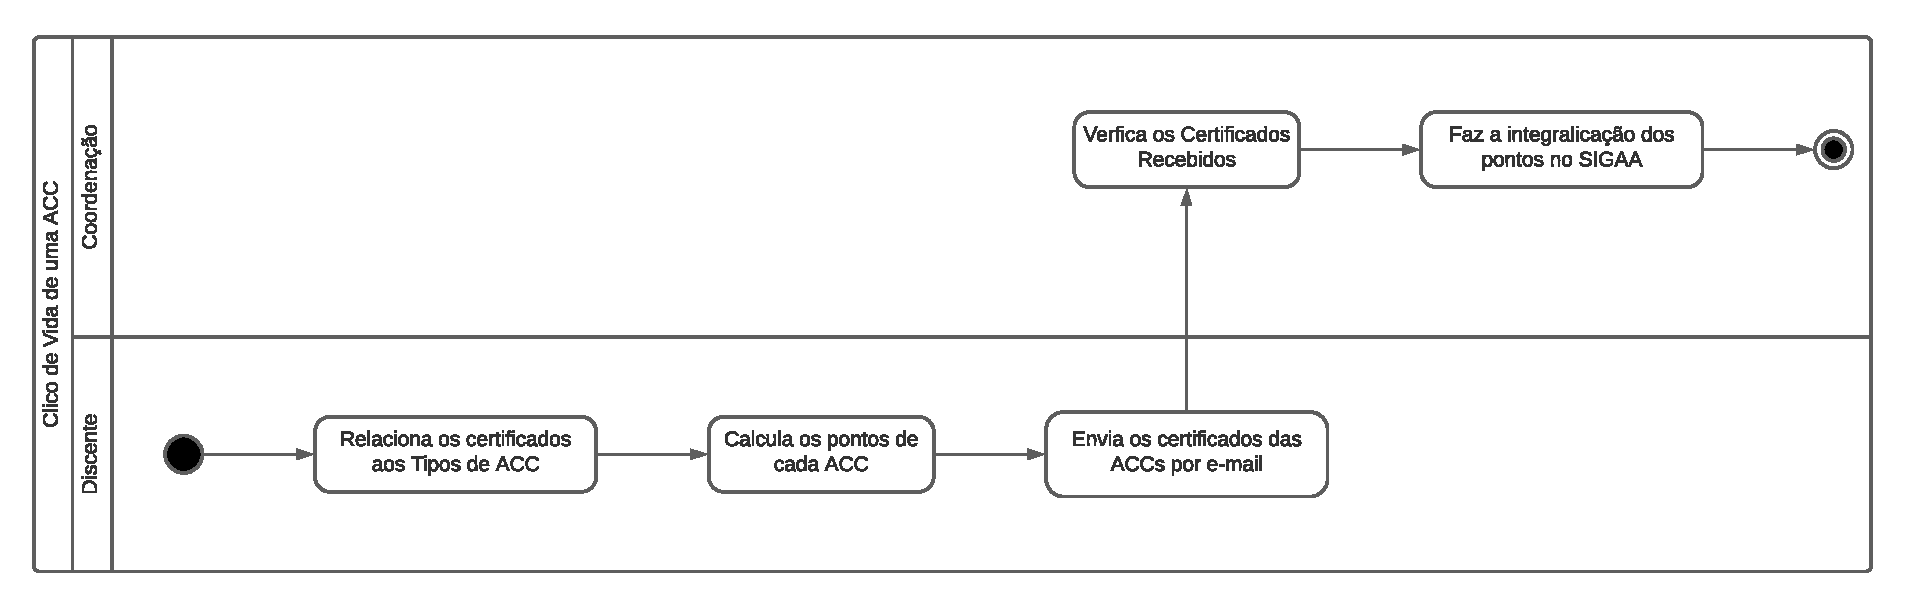
\includegraphics[width=\textwidth]{dados/figuras/Referencial Teórico/avaliacao_acc_manual.pdf}
    \caption{Fluxo de Avaliação de uma ACC}
    \label{fig:fluxoAvaliacaoDeACC}
\end{figure}         % Revisão de Literatura

\chapter{TRABALHOS RELACIONADOS}
\label{chap:trabalhosrelacionados}

Existem na literatura vários trabalhos que focam no desenvolvimento de sistemas para a gestão da informação e de atividades curriculares complementares.
A seção \ref{sec:gestacademic} abordará trabalhos em gestores de informação voltados ao ambiente de aprendizado. Enquanto a seção \ref{sec:gestativcomplem} mostrará gestores de Atividades Curriculares Complementares, e que possuem o mesmo foco da ferramenta proposta.

\section{Gestores de Informação}
\label{sec:gestacademic}

\cite{cardoso2018desenvolvimento} aborda em seu trabalho as etapas da criação da ferramenta SAAMS (Sistema de Assistência Estudantil e Acompanhamento Acadêmico), desenvolvida mediante uma necessidade da Coordenadoria de Acompanhamento Acadêmico (CAAd) do Instituto
Federal do Rio Grande do Sul (IFRS). Conforme descrito por \cite{cardoso2018desenvolvimento}, todos os processos da CAAd eram realizados através de planilhas, ou até mesmo com arquivos de texto. Tal abordagem não era ideal, pois acabava gerando operações repetitivas e informações conflitantes ou inconsistentes. Diante disso, foi necessária a criação de uma ferramenta que auxiliasse nos processos da CAAd. \cite{cardoso2018desenvolvimento} descreve então as etapas do processo necessárias para a criação da ferramenta, desde a etapa de levantamento de requisitos até a codificação em si da aplicação.

Em \cite{barroca2013sigaa} é mostrado o processo de implantação de uma versão voltada para dispositivos móveis do Sistema Integrado
de Gestão de Atividades Acadêmicas (SIGAA) na Universidade Federal do Rio Grande do Norte (UFRN). Segundo \cite{barroca2013sigaa} havia uma necessidade de se atender à demanda crescente de dispositivos móveis com a criação de uma aplicação voltada a estes, porém esta aplicação deveria manter as funcionalidades já presentes no sistema, de forma que qualquer ação realizada pelo sistema em si pudesse ser realizada por um dispositivo móvel. O trabalho aborda as etapas que foram seguidas na criação da aplicação, desde a modelagem até a codificação em si. \cite{barroca2013sigaa} demonstra ainda uma avaliação dos resultados que mostraram um grande número de instalações em proporção ao número total de usuários do sistema.

Em seu trabalho \cite{gomes2012genome} descrevem a utilização da ferramenta GENOME que trabalha em consonância com o Moodle, um sistema livre de apoio ao aprendizado, para se fazer a avaliação da participação virtual e gerenciamento de notas dos discentes do Instituto Metrópole Digital da Universidade Federal do Rio Grande do Norte (UFRN). \cite{gomes2012genome} explica que a avaliação das notas dos alunos é feita levando em consideração tanto as atividades realizadas presencialmente,  que englobam presença, pontualidade,
resolução de exercícios, participação no encontro, seminários e questões desafios, quanto as realizadas à distância, como a participação de fóruns e chats. Todas essas avaliações são avaliadas e juntas compõem a nota final, o GENOME serve então como uma ferramenta que faz a padronização dessas avaliações, e cria relatórios mais completos do que os já existentes dentro da ferramenta Moodle.

% O trabalho de \cite{amin2018active} tem um viés mais técnico em relação aos sistemas abordados descreve a criação de uma abordagem de sistema de banco de dados para o desenvolvimento de uma aplicação de gestão acadêmica. Um Banco de Dados Ativo é descrito como capaz de capturar determinados eventos e realizar ações a partir disso. O sistema também faz o uso de regras, que são descritas como uma complementação de uma linguagem de programação utilizada no desenvolvimento de uma aplicação.

% No trabalho de \cite{sankar2018web} é descrito o desenvolvimento de uma aplicação para o gerenciamento acadêmico, visando automatizar as ações realizadas no ambiente acadêmico e assim eliminando os problemas gerados pela operação manual dessas ações. A aplicação foi desenvolvida em ASP e permite que os alunos possam ter aulas através dela.


\cite{rodriguez2018desenvolvimento} apresentam em seu trabalho a criação da ferramenta SolicitaUFF, um sistema acadêmico-administrativo com foco em usabilidade e acessibilidade. Segundo \cite{rodriguez2018desenvolvimento}, até então os processos desempenhados pela coordenação da Universidade Federal Fluminense (UFF) eram em grande parte feitos de forma manual, e os alunos precisavam comparecer à coordenação para realizar ações como: requerimentos de Atividades Complementares; dispensa em disciplinas; entre outras. A criação do sistema teve como foco aumentar a eficácia dos processos da UFF através da informatização dos processos, e assim diminuir o tempo perdido na execução manual dos mesmos.

\section{Gestores de Atividades Curriculares Complementares}
\label{sec:gestativcomplem}

\cite{de2018implementaccao} discorrem sobre o desafio das Instituições de Ensino Superior em fazer o controle das Atividades Complementares realizadas pelos discentes e ainda de tornar esse controle transparente. As Instituições utilizam diferentes estratégias, seja utilizando correio eletrônico, comparecimento presencial do discente ou um sistema específico, porém esse processo é desafiante no que tange a permitir que os discentes tenham um acompanhamento claro de seus avanços. \cite{de2018implementaccao} descrevem então sobre a criação da ferramenta \textit{Akademic} que seria uma ferramenta de Gestão de Atividades Complementares utilizável por qualquer Instituição.

\cite{silva2013processo} demonstram em seu trabalho a utilização da ferramenta Moodle, um ambiente virtual de aprendizado, para o gerenciamento das Atividades Complementares dos discentes da  Faculdade de Computação e Informática (FCI) da Universidade Presbiteriana Mackenzie (UPM). \cite{silva2013processo}. Através da utilização dessa ferramenta acarretou a diminuição da utilização de papel na FCI, além da criação de um canal onde alunos e professores poriam colaborar em discussões, e onde os alunos poderiam ter acesso às atividades da Faculdade.


\cite{cunha2014unipampa} explica que há um desafio no controle das Atividades Curriculares de Graduação (ACGs) na Universidade Federal do Pampa (UNIPAMPA), pois o processo de aproveitamento das ACGs é trabalhoso, exigindo que os discentes preencham a requisição desse aproveitamento, relacionando suas atividades com a tabela de ACGs da UNIPAMPA. O maior desafio está no fato de que os discentes muitas vezes esperam até o último período para fazer esse aproveitamento, gerando atrasos nessas requisições. Diante desse cenário \cite{cunha2014unipampa} descreve sobre a criação da ferramenta SmartACG que tem como objetivo a informatização dos processos de integralização de ACGs, dessa forma a ferramenta seria um automatizador de processos, que auxiliaria os alunos na integralização das ACGs.

Com o objetivo de relacionar as especificidades de cada ferramenta foi feita uma comparação entre eles, que pode ser encontrada na Tabela \ref{table:ComparacaoArtigos}, essa comparação também envolve o KeeMe, ferramenta desenvolvida neste trabalho. As seguintes características serão abordados na tabela:

\begin{itemize}
    \item \textbf{Plataformas:} Descreve quais as plataformas são abarcadas pelo sistema, ou seja, se ele é Web ou Móvel;
    \item \textbf{\textit{Status}:} Aborda a capacidade que o sistema tem de mostrar aos alunos se suas ACCs foram avaliadas, aprovadas ou reprovadas;
    \item \textbf{Personalização:} Descreve o tipo de personalização que cada tipo de ACC possuirá. Os campos avaliados são: Nome, que descreve o nome do tipo de ACC; Peso, relativo, por exemplo à quantidade de horas que são necessárias para que se consiga um ponto de ACC; e Limite, que é a pontuação máxima que um usuário poderá conseguir com determinado tipo de ACC.
\end{itemize}

\begin{table}[H]
\centering
\caption{Tabela comparativa dos trabalhos relacionados com a proposta.}
\label{table:ComparacaoArtigos}
\begin{tabular}{|C{3.64cm}|C{3.14cm}|C{2.78cm}|C{4.64cm}|}
\hline
\textbf{Ferramenta} & \textbf{Plataformas} & \textbf{\textit{Status}} & \textbf{Personalização} \\
\hline
Akademic & Web & Não  & Nome da ACC \\ \hline
Moodle & Web & N/A & Nome da ACC \\ \hline
SmartACG & Móvel & Sim & Nome da ACC \\ \hline
KeeMe & Web & Sim & Nome da ACC, Peso e Limite \\ \hline
\end{tabular}
\end{table}

A ferramenta Akademic de \cite{de2018implementaccao} é a mais próxima da solução proposta neste trabalho em questões de interface do usuário e usabilidade, permitindo que o usuário utilize o sistema tanto em um computador quanto em um celular sem limitações de funcionalidade, porém tem como limitações a utilização apenas de Horas para avaliar o avanço das ACCs, e da não conversão dessas horas em pontos, o que é algo essencial para a avaliação de ACCs na FACEEL. O trabalho de \cite{cunha2014unipampa}, possui a limitação de ser criado apenas para a plataforma Android, sem a possibilidade de acesso por um computador, e sem acesso pelos coordenadores. Já \cite{silva2013processo} apesar de também se tratar de uma ferramenta de informatização das ACCs, possui a limitação de ser baseado na plataforma Moodle, restringindo seu uso pelos discentes da FACEEL.




% Metodologia
% MATERIAIS E MÉTODOS------------------------------------------------------------------

\chapter{MATERIAIS E MÉTODOS}
\label{chap:metodologia}
Neste capítulo serão descritos os materiais e métodos utilizados no desenvolvimento da aplicação KeeMe, bem como as tecnologias que foram empregadas em sua construção. A Seção \ref{sec:desenvolvimento} descreve o processo de desenvolvimento utilizado na criação da ferramenta, discorrendo sobre as etapas do desenvolvimento e o que foi feito em cada uma delas. Já a Seção \ref{sec:gerenciamentoDaAplicacao} abordará a metologia que foi utilizada para fazer o gerenciamento do projeto como um todo. Na Seção \ref{sec:modelagem} será descrita a modelagem da aplicação, e aborda a UML, linguagem visual para modelagem e quais de seus recursos foram usados no desenvolvimento dessa aplicação. A Seção \ref{sec:prototipacao} discorrerá sobre a etapa de prototipação da interface do sistema e da estratégia utilizada para tanto. E por último, a Seção \ref{sec:tecnologias} discorrerá sobre tecnologias que foram utilizadas na criação da ferramenta.

\section{Processo de Desenvolvimento}
\label{sec:desenvolvimento}

\begin{figure}[H]
    \centering
    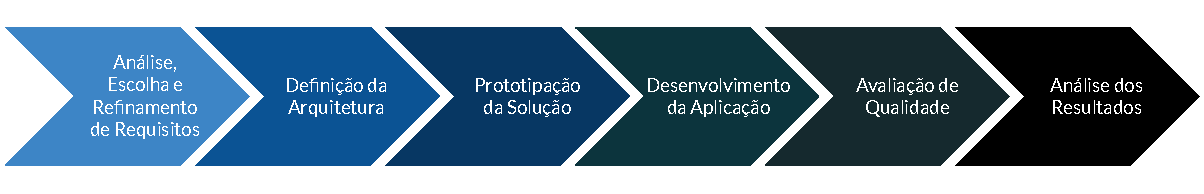
\includegraphics[width=\textwidth]{dados/figuras/Metodologia/grafico_evolutivo.pdf}
    \caption{Processo de desenvolvimento}
    \label{fig:processoDeDesenvolvimento}
\end{figure}

Durante o decorrer deste trabalho foi utilizado um Modelo Incremental para o seu desenvolvimento, descrito por \cite{dias2019__modelo_incremental} como uma evolução do Modelo Cascata, no qual ao invés de se especificar e desenvolver tudo de uma só vez, são feitas pequenas entregas, na forma de incrementos. A Figura \ref{fig:processoDeDesenvolvimento} mostra o processo descrito.

A etapa de Análise, Escolha e Refinamento de Requisitos serve para se coletar os requisitos do sistema das partes interessadas, esses requisitos serão importantes na construção das funcionalidades da aplicação; A etapa de Definição da Arquitetura está relacionada à criação da documentação da aplicação, como diagramas de caso de uso, mapas conceituais, etc; Já a etapa de Prototipação da Solução é utilizada para se criar um protótipo não funcional da aplicação, que serverá como referencial na etapa de desenvolvimento; No Desenvolvimento da Aplicação é feita a codificação da aplicação utilizando a arquitetura e o protótipo criados anteriormente; Após isso, é feita a Avaliação de Qualidade das funcionalidades criadas, através de testes de performance, acessibilidade entre outros; E por último é feita a Análise dos Resultados gerados pela Avaliação de Qualidade.

\section{Gerenciamento da Aplicação}
\label{sec:gerenciamentoDaAplicacao}

Durante a fase de codificação da aplicação, foi utilizada uma abordagem baseada no Kanban, utilizando o Trello para fazer o gerenciamento daquilo que já havia sido desenvolvido e do que ainda precisava ser feito na aplicação.
Segundo \cite{mesh2020__metodo_kanban} o Kanban pode ser visto como um "método visual para gerenciar e conduzir o trabalho", e visa a simplificação do gerenciamento das tarefas, mostrando através da utilização de cartões quem está executando qual tarefa. \cite{trello} explica que o Trello é uma ferramenta de gestão de projetos que auxilia os times a agilizarem o trabalho, o Trello baseia-se no Kanban, utilizando a estratégia de cartões e raias para fazer o gerenciamento dos projetos.

\begin{figure}[H]
    \centering
    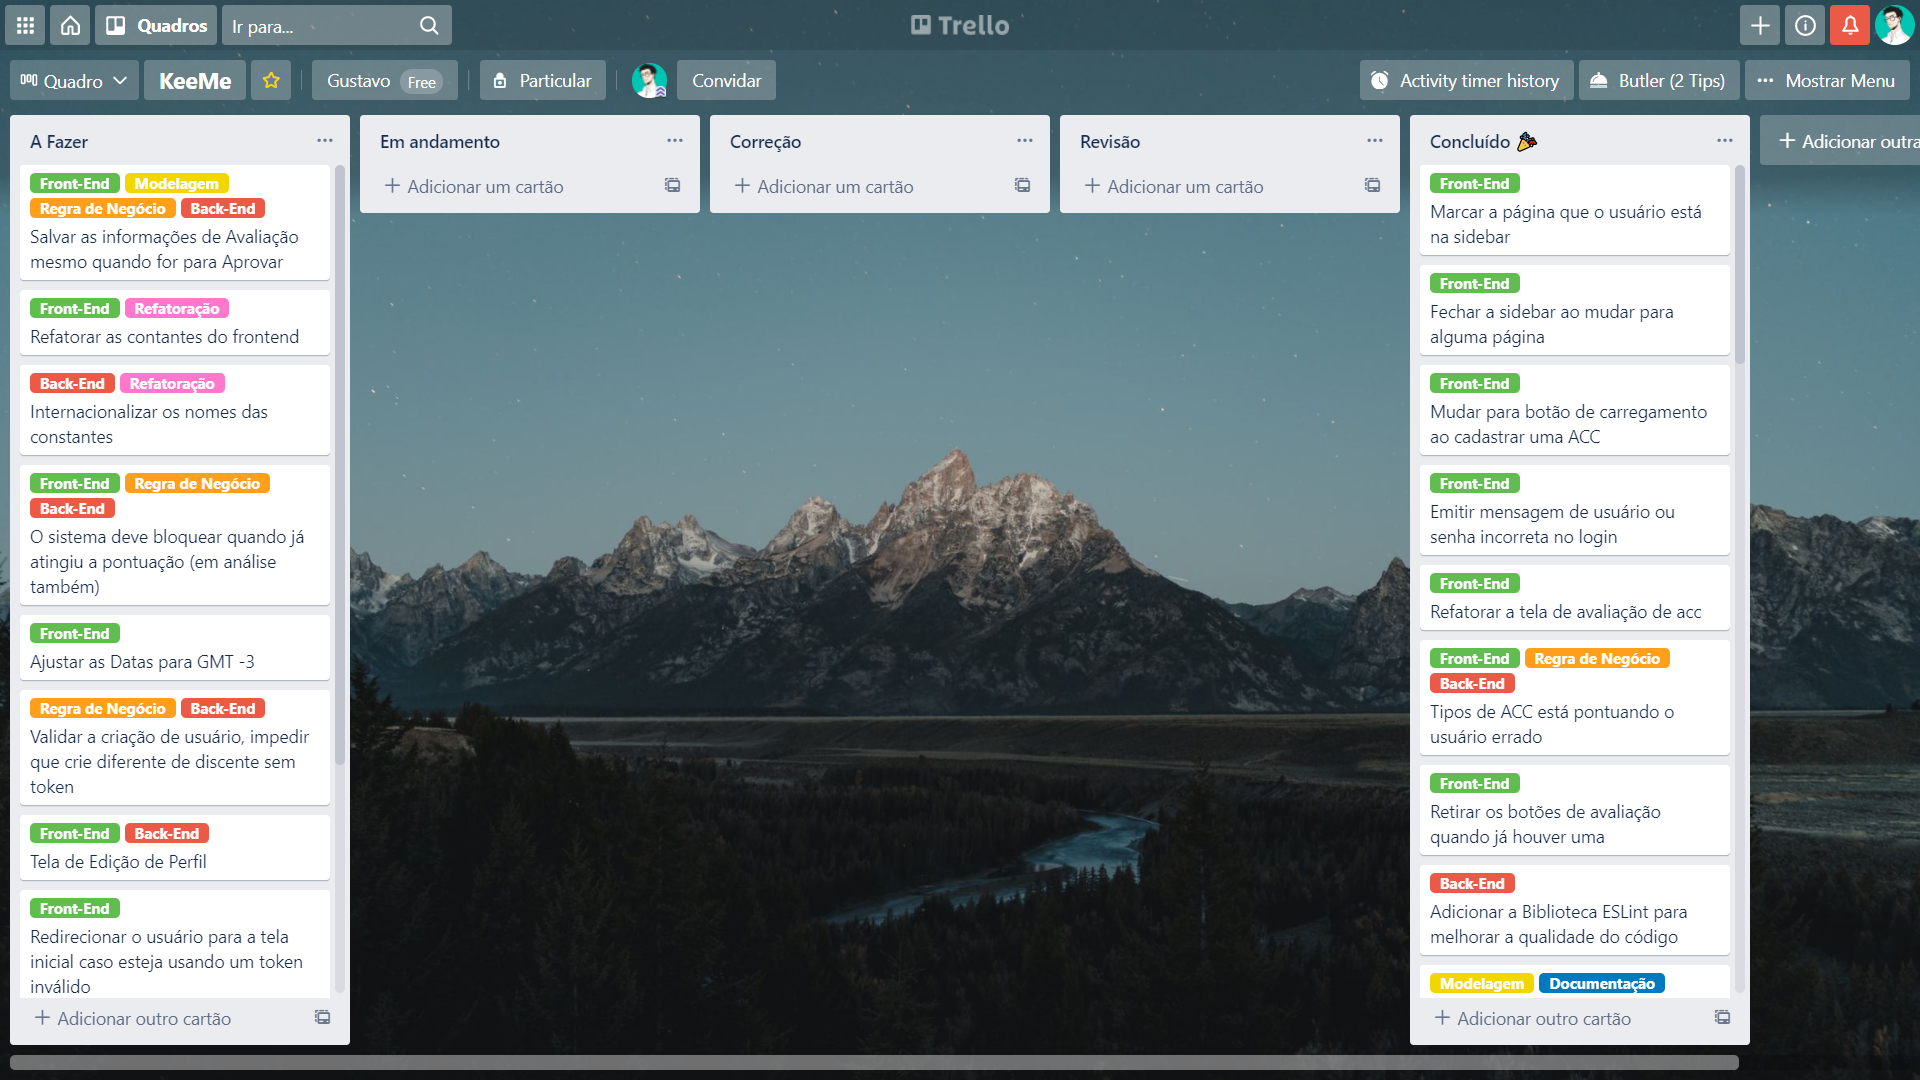
\includegraphics[width=\textwidth]{dados/figuras/Metodologia/trello.png}
    \caption{Quadro no Trello do Projeto KeeMe}
    \label{fig:screenTrelloKeeMe}
\end{figure}

A Figura \ref{fig:screenTrelloKeeMe} mostra o quadro do Trello utilizado no projeto KeeMe. No projeto foram utilizadas 5 colunas, sendo estas: A Fazer, que relaciona todas as tarefas que ainda precisam ser implementadas na aplicação; Em andamento, que é aquilo que está sendo executado no momento; Correção, que reune as tarefas que foram feitas, mas nos quais foram encontradas bugs, ou que não foram desenvolvidas corretamente; A coluna de Revisão, que é aquilo que deve ser testado; E por último a coluna de Concluído, que reúne todas as tarefas que foram executadas, e que foram concluídas da conforme o planejado.

Além da utilização de raias, conforme pode ser visto na \ref{fig:screenTrelloKeeMe}, foram utilizadas também as etiquetas coloridas para melhorar o gerenciamento das tarefas e ter um auxílio visual da área ao qual a tarefa pertence, as etiquetas utilizadas são: \textit{Front-end}, que descreve tudo que deve ser feito da parte visual do sistema; \textit{Back-end}, que é o serviço onde estão as regras de negócio do sistema; Regra de negócio, essa etiqueta se refere a qualquer tarefa que esteja diretamente ligada à regra de negócio, como as pontuações, por exemplo; Modelagem, que diz respeito às tarefas de modelagem dos processos e do banco de dados; Prototipação, que relaciona-se à parte visual do sistema, à tudo que envolva o protótipo do projeto; Documentação, como o nome sugere, é a parte da escrita de documentos relativos ao código, arquitetura, etc, do sistema; Infraestrutura, são tarefas relativas à integração com banco de dados, à hospedagem do site e à forma que os serviços (\textit{Front-end} e \textit{\textit{Back-end}}) da aplicação se comunicam; Refatoração, que é tudo aquilo que foi feito e está funcional, mas que de alguma forma precisa ser melhorado; e por último Banco de Dados, que está diretamente ligado à modelagem e ao \textit{Back-end}, e diz respeito a tudo que envolva o banco de dados da aplicação.

\section{Modelagem}
\label{sec:modelagem}

A modelagem de sistemas serve para que se tenha uma direção clara do que se fazer durante o desenvolvimento da aplicação. A criação de diagramas e modelos serve para que os desenvolvedores saibam exatamente o que deve ser feito, quais as entidades de uma aplicação e como essas entidades relacionam-se entre si, quais os fluxos de funcionalidades, entre outros aspectos inerentes à aplicação sendo desenvolvida. É um fator indispensável na busca pela qualidade na criação de um software.

Para se realizar a modelagem foi utilizada a UML (Unified Modeling Language), segundo \cite{guedes2018uml}, é uma linguagem visual utilizada para modelar softwares baseados no paradigma de orientação a objetos. O UML surge como uma linguagem amplamente utilizada de modelagem, tornando-se o padrão de qualquer equipe de desenvolvimento, e sendo extremamente útil na fase de planejamento de um software. \cite{guedes2018uml} ressalta que a UML não se trata de uma linguagem de programação, além de também não ser um processo de desenvolvimento.

\section{Prototipação}
\label{sec:prototipacao}

A etapa de prototipação do sistema se deu para que fosse possível ser ter uma direção ao qual seguir em relação à interface da aplicação. Dessa forma, assim como se faz necessária a modelagem do banco de dados de uma aplicação de forma a se planejar a interação entre as classes e métodos, também se faz necessária a prototipação da interface da aplicação. Para fazer a modelagem do KeeMe foi utilizada a ferramenta Figma, uma ferramenta de design de interface na qual todo o trabalho é feito através do navegador \cite{interativa2019figma}.

\begin{figure}[H]
    \centering
    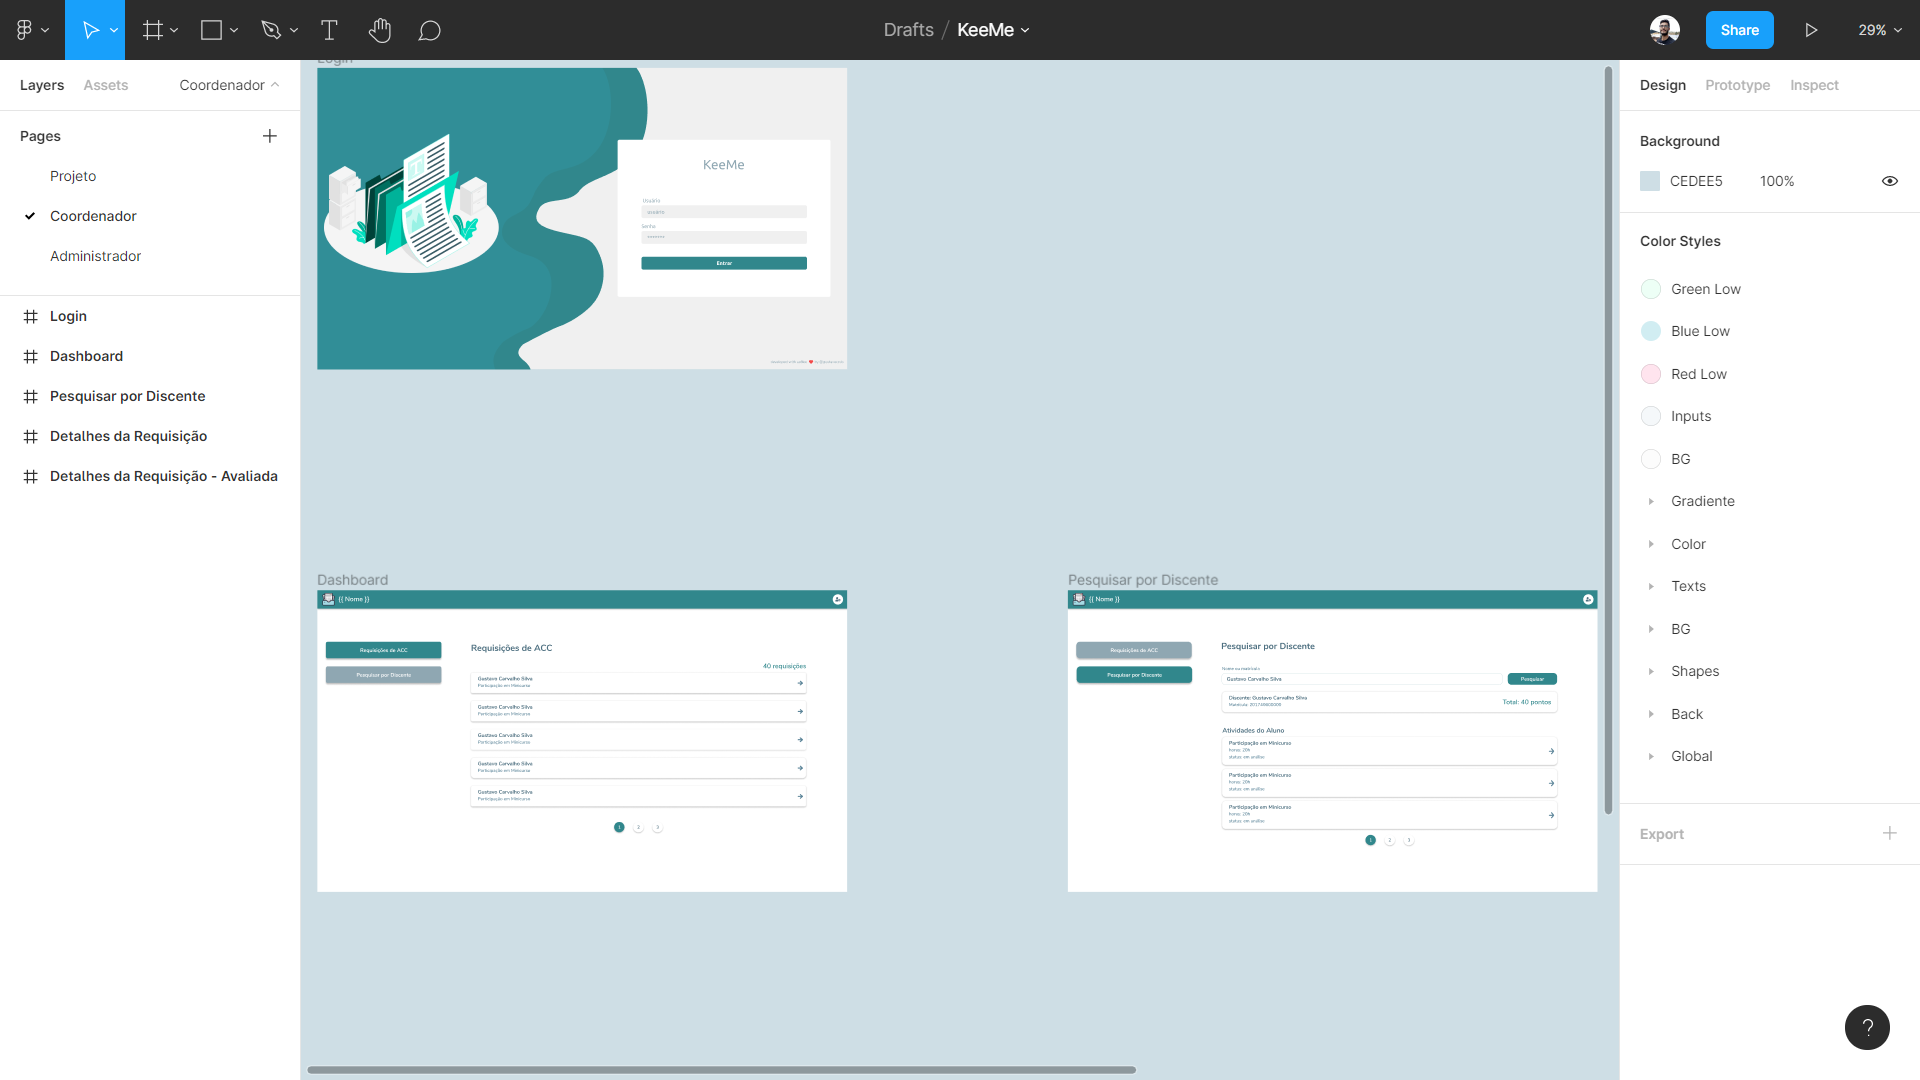
\includegraphics[width=\textwidth]{dados/figuras/Metodologia/figma.png}
    \caption{Prototipo do Projeto KeeMe}
    \label{fig:figmaKeeMe}
\end{figure}

A Figura \ref{fig:figmaKeeMe} mostra um exemplo das telas criadas na prototipação. Neste caso, estão sendo exibidas três telas do módulo do Coordenador, que são as telas de Login, Início e Pesquisa de Discente. 

A utilização de um protótipo permitiu uma melhor visualização da aplicação final, além de servir como um norteador do que deveria ser criado, e do que poderia ser utilizado dentro da aplicação. Após concluído o protótipo\footnote[1]{https://www.figma.com/file/28fcRaEdbWgQkIAw6Pnfwh/KeeMe?node-id=0\%3A1}, foi realizada uma reunião junto à comissão responsável pelo regulamento de ACCs, composta por dois professores e um aluno representante de cada curso da FACEEL. Através dessa reunião a interface, assim como as funcionalidades que ela deveria possuir, foram validadas e aprovadas, permitindo o início da codificação baseada no protótipo.

\section{Tecnologias}
\label{sec:tecnologias}

As tecnologias utilizadas na concepção de um software tem ligação direta com o funcionamento final da aplicação. Dessa forma, a escolha do conjunto de ferramentas deve ser feita com cuidado, considerando o escopo do software desenvolvido.

A modelagem dos diagramas mostrando as relações entre entidades do sistema e dos fluxos de processos foi feita utilizando a aplicação LucidChart descrita por \cite{lucidchart} como sendo uma ferramenta de criação de diagramas inteligentes. Tal escolha se deu pela facilidade na utilização da ferramenta, o que diminuiu a curva de aprendizado, e pelas funcionalidades que a ferramenta apresenta em relação à criação de diagramas.

Tanto o \textit{Back-end} quanto o \textit{Front-end} da aplicação foram construídos utilizando o Node.js como base, como descrito em \cite{node} o Node.js é uma ferramenta que permite a execução de código Javascript, linguagem descrita em \cite{javascript} como uma linguagem linguagem leve, interpretada e baseada em objetos mais conhecida como linguagem de \textit{scripts} para web, sem a necessidade de um navegador. O código do projeto foi escrito em Typescript, que por sua vez é descrito em \cite{typescript} como um superconjunto de Javascript que adiciona novas funcionalidades à linguagem, dentre essas funcionalidades a mais importante é a de tipagem dos dados, algo não existente no Javascript, e que permite um controle melhor das informações que estão sendo manipuladas na aplicação, além da capacidade de criar implementações utilizando programação orientada a objetos no Javascript. Como editor de código, foi escolhido o Visual Studio Code ferramenta desenvolvida pela Microsoft e descrito como um "um editor de código-fonte leve, mas poderoso, que roda em sua área de trabalho e está disponível para Windows, macOS e Linux" \cite{visualstudiocode}.

Como base de dados, foi utilizado o MySQL que segundo \cite{mysql} é um banco de dados que possui bom desempenho, confiabilidade e facilidade de uso, tal escolha se deu pela necessidade da utilização de um banco de dados relacional, que é descrito por \cite{oracle2021bancorelacional} como sendo um tipo de banco de dados que armazena e fornece acesso a pontos de dados relacionados entre si, e que faz a utilização de tabelas e chaves para fazer as relações entre as informações armazenadas. Todas as operações de manipulação de dados do banco e do banco de dados em si são feitas usando a biblioteca TypeORM, descrito em \cite{typeorm} como um ORM (Object-relational mapping, "Mapeamento objeto-relacional") que tem como objetivo trazer suporte às últimas funcionalidades do Javascript, provendo funcionalidades que auxiliam na criação de aplicações que utilizam banco de dados, um ORM é descrito por \cite{fonseca2019orm} como sendo um paradigma de aproximação dos bancos de dados relacionais com a programação orientada a objetos. Para auxiliar na visualização do banco de dados foi utilizado o BeeKeeper Studio, um "gerenciador e editor de SQL de código aberto" \cite{beekeeper}.

O \textit{Front-end} da aplicação foi construído utilizando o React, biblioteca criada por \cite{react} com o foco na construção de interfaces e que permite a manipulação de elementos HTML dentro do Javascript. O React foi escolhido primeiramente pela popularidade da biblioteca, o que impacta na quantidade de documentação e de extensões criadas para a mesma; e pela capacidade de componentização do código, que permite sua reutilização dentro do software, diminuindo o re-trabalho. Em conjunto ao React foi utilizado o \textit{framework} ChakraUI, que de acordo com \cite{chakraui} se trata de uma biblioteca de componentes de interface, a escolha deste \textit{framework} se deu pelo fato de que além de possuir componentes de layout prontos, também permite a personalização desses componentes, facilitando a estilização do software.

Além das tecnologias já citadas, foram utilizados também o Insomnia, que segundo sua documentação em \cite{insomnia} é uma ferramenta de código aberto que permite a chamada de requisições REST, e foi utilizada durante o desenvolvimento para os testes nos serviços providos pelo \textit{Back-end} da aplicação. O REST segundo \cite{costa2020__rest} é um padrão arquitetural de informações trafegadas entre dois diferentes sistemas através de uma rede de internet; A ferramenta Git para o versionamento do código gerado, \cite{git} explica que o Git é uma ferramenta de versionamento de código, que pode ser utilizada desde projetos pequenos, quanto projetos complexos com rapidez e eficiência. O Git permite o rastreamento de alterações no código, comparações com versões anteriores, e permite desfazer alterações que possam ter causado erro no código; Foi utilizado ainda o Lighthouse, uma ferramenta de desenvolvedor de código aberto, que segundo \cite{lighthouse} possui a capacidade de fazer testes automatizados numa página web para avaliar sua qualidade. A ferramenta foi utilizada para avaliar o grau de qualidade da aplicação desenvolvida neste trabalho.
 

% Proposta
\chapter{SISTEMA WEB KEEME} 
\label{chap:proposta}

O KeeMe (Keep it to Me, "Guarde isso para mim") nasceu de uma necessidade da Faculdade de Computação e Engenharia Elétrica de informatizar o processo de validação das ACCs realizadas pelos discentes. Dessa forma, o sistema fará o armazenamento dos certificados gerados pelos discentes, e calculará os pontos gerados por essas ACCs. O objetivo principal da ferramenta é simplificar o processo de validação dos certificados por parte da faculdade, diminuindo a burocracia necessária para a avaliação, e dar aos discentes um acompanhamento de quantos pontos eles já obtiveram e em quais modalidades de ACCs eles podem adquirir mais pontos.

A Seção \ref{sec:coleta_de_requisitos} descreverá a etapa de coleta e análise de requisitos do sistema, feita com as partes interessadas do sistema. Já a Seção \ref{sec:modelagemDeRequisitos} irá discorrer sobre a etapa de modelagem dos requisitos coletados em representações gráficas. A arquitetura do sistema será mostrada na Seção \ref{sec:arquiteturaDoSistema} que explicará a forma em que o sistema foi estruturado. E por último a Seção \ref{sec:implementacao} explanará sobre a implementação da ferramenta, mostrando as funcionalidades que foram criadas.

\section{Coleta de Requisitos}
\label{sec:coleta_de_requisitos}

O autor de \cite{pmbok2017} descreve a etapa de coleta e análise de requisitos como "o processo de determinar, documentar e gerenciar as necessidades e requisitos das partes interessadas a fim de cumprir os objetivos". Dessa forma, requisitos de um software são todas as necessidades que as partes interessadas possuem dentro de um determinado escopo e que devem ser resolvidas através do desenvolvimento de uma aplicação. Através de reuniões e da análise do documento referente à pontuação de carga horária de ACCs que pode ser encontrado no Anexo \ref{anexo:novaResolucaoDeACC}, foram elencados requisitos funcionais e não funcionais, listados de acordo com o grau de prioridade.

Os requisitos levantados foram divididos entre requisitos funcionais, que de acordo com \cite{pmbok2017} descrevem os comportamentos do produto, ou seja, são as ações diretas que os usuários do sistema realizarão e a forma que o sistema reagira a elas; e não funcionais, são todos aqueles em que não há interação direta por parte do usuário, e que estão relacionados à infraestrutura por trás da aplicação, descritos como uma complementação dos requisitos funcionais que descrevem as condições ou qualidades ambientais requeridas para que o produto seja eficaz.

A Tabela \ref{table:RequisitosFuncionais} lista a relação dos requisitos funcionais coletados. Os requisitos estão classificados por ordem de prioridade como "essencial" sendo algo que deve obrigatoriamente ser desenvolvido no sistema, "importante" como algo que agregaria mais valor ao sistema, mas que não interfere na utilização e "desejável" como sendo algo além daquilo que a aplicação já se propõe a fazer, e que não interfere de forma alguma em seu funcionamento.

\begin{table}[H]
\centering
\caption{Requisitos Funcionais}
\label{table:RequisitosFuncionais}
\begin{tabular}{|C{1.2cm}|C{11.2cm}|C{2.2cm}|}
\hline
\textbf{ID} & \textbf{Descrição} & \textbf{Prioridade} \\
\hline
RF 1 & O usuário poderá fazer login no sistema. & Essencial \\ \hline
RF 2 & O discente poderá gerenciar as pontuações dos respectivos ACCs. & Essencial \\ \hline
RF 3 & O discente poderá enviar os certificados digitalmente pela plataforma. & Essencial \\ \hline
RF 4 & O sistema mostrará aos discentes o seu progresso na obtenção das ACCs. & Essencial \\ \hline
RF 5 & A pontuação do discente deverá obedecer os limites de cada tipo de ACC. & Essencial \\ \hline
RF 6 & A coordenação do curso poderá acompanhar as ACCs de cada discente. & Essencial \\ \hline
RF 7 & A coordenação do curso poderá validar os documentos enviados pelos discentes. & Essencial \\ \hline
RF 8 & A administração poderá gerenciar os dados referentes a ACC (pontuação, carga máxima, etc). & Importante \\ \hline
RF 9 & A coordenação poderá cadastrar o motivo caso um certificado de ACC seja negado. & Desejável \\ \hline
RF 10 & A coordenação poderá acompanhar o desempenho geral por turma na obtenção de ACC & Desejável \\ \hline
RF 11 & A coordenação poderá fazer a geração de relatórios das pontuações dos alunos & Desejável \\ \hline

\end{tabular}
\end{table}


Os requisitos não funcionais coletados e relacionados na Tabela \ref{table:RequisitosNaoFuncionais}, assim como os funcionais, estão classificados por ordem de prioridade como "essencial" sendo algo que deve obrigatoriamente ser desenvolvido no sistema e que é essencial para o seu funcionamento, "importante" como algo que agregaria mais valor ao sistema, mas que não interfere diretamente no seu funcionamento final, e "desejável" como sendo algo que poderia ser implementador na arquitetura da aplicação, porém não interfere de forma alguma em seu funcionamento final.

\begin{table}[H]
\centering
\caption{Requisitos Não Funcionais}
\label{table:RequisitosNaoFuncionais}
\begin{tabular}{|C{1.2cm}|C{11.2cm}|C{2.2cm}|}
\hline
\textbf{ID} & \textbf{Descrição} & \textbf{Prioridade} \\
\hline
RNF 1 & O sistema deverá possuir autenticação e uso de \textit{tokens} de forma a garantir a segurança dos usuários. & Essencial \\ \hline
RNF 2 & O deverá possuir criptografia das senhas dos usuários. & Essencial \\ \hline
RNF 3 & O sistema deverá estar disponível a todo momento. & Essencial \\ \hline
RNF 4 & O sistema deverá ser responsivo, com foco na utilização em dispositivos móveis. & Essencial \\ \hline
RNF 5 & O sistema deverá ter suporte para os principais navegadores, sendo estes: Chrome, Firefox, Safari, Microsoft Edge. & Importante \\ \hline
RNF 6 & Deverão ser seguidas as principais heurísticas de Interface Homem Computador de forma a garantir a usabilidade do sistema. & Importante \\ \hline
RNF 7 & Deverá haver o suporte a um PWA do sistema & Desejável \\ \hline
RNF 8 & Deverá possuir código HTML escrito de forma semântica de forma a permitir acessibilidade. & Desejável \\ \hline

\end{tabular}
\end{table}

\section{Modelagem de Requisitos}
\label{sec:modelagemDeRequisitos}

O objetivo da etapa de modelagem de requisitos é transformar os requisitos coletados pelas partes interessadas em artefatos que sejam compreensíveis visualmente à equipe de desenvolvimento. \cite{pressman2009engenharia} descreve a modelagem como sendo algo que ”abrange tanto análise quanto projeto, descrevendo representações do \textit{software} que se tornam progressivamente mais detalhadas”. Essas representações são essenciais para que se saiba exatamente o que se deve ser desenvolvido dentro de um \textit{software}.

\subsection{Casos de Uso de Alto Nível e Expandido}

O autor \cite{guedes2018uml} descreve os casos de uso como diagramas que procuram por meio de uma linguagem simples demonstrar as funcionalidades de um sistema para os usuários, possibilitando uma melhor compreensão por parte daqueles que não entendem completamente o funcionamento interno do sistema. Diagramas de caso de uso servem então para mostrar quais são os atores de um sistema, sendo esses atores os tipos de usuários, e quais as ações que cada um desses atores podem realizar. Dentro do contexto do KeeMe, existem os seguintes atores:
\begin{itemize}
    \item Discente: é o ator que representa um discente no sistema, ele possui a capacidade de fazer a gestão das ACCs assim como de visualizar a pontuação que já obteve.
    \item Coordenador: usuário capaz de realizar as avaliações de ACC dentro do sistema, assim como de visualizar as pontuações dos alunos.
    \item Administrador: é o usuário que faz o gerenciamento dos tipos de ACC presentes no sistema, assim como dos coordenadores;
\end{itemize}

\begin{figure}[H]
    \centering
    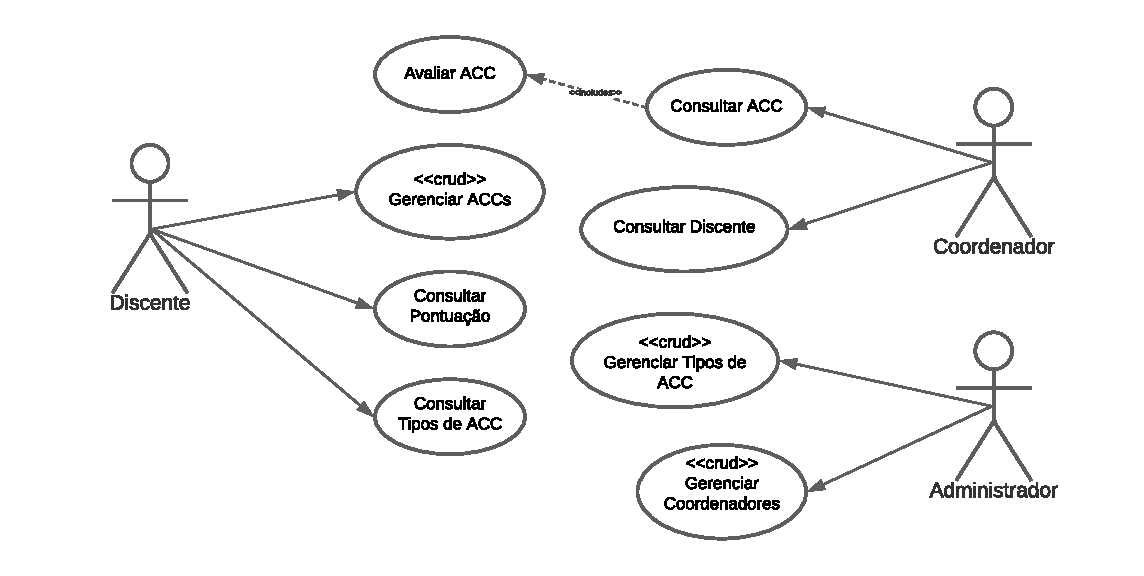
\includegraphics[width=\textwidth]{dados/figuras/Proposta/casos_de_uso_de_alto_nivel__keeme.pdf}
    \caption{Diagrama de Caso de Uso de Alto Nível do KeeMe.}
    \label{fig:casoDeUsoAltoNivel}
\end{figure}

Os casos de uso também podem ser expandidos textualmente em uma sequência de passos presentes dentro dos mesmos. A Tabela \ref{casoExpandido:consultarPontuacao} descreve o caso de uso onde o discente faz a consulta de sua pontuação no sistema, essa pontuação é referente à pontuação necessária para integralização da matéria de ACC; Já a Tabela \ref{casoExpandido:consultarTiposDeACC} demonstra a sequência de ações presentes no caso de uso de consulta dos tipos de ACC, onde o discente poderá acessar os tipos de ACC presentes no sistema; A Tabela \ref{casoExpandido:gerenciarACCs} também é referente às ações do discente, e diz respeito às ações de cadastro, consulta, edição e exclusão das ACCs de um discente.

Os casos de uso de um usuário do tipo coordenador estão listados nas Tabelas \ref{casoExpandido:consultarACC}, \ref{casoExpandido:avaliarACCs} e \ref{casoExpandido:consultarDiscentes}. A Tabela \ref{casoExpandido:consultarACC} descreve a consulta de uma ACC, onde o coordenador poderá acessar os detalhes de uma ACC enviada por um discente; Já a Tabela \ref{casoExpandido:avaliarACCs} descreve a sequência de passos para a avaliação de uma ACC, como mostrado na Figura \ref{fig:casoDeUsoAltoNivel} essa ação inclui o caso de uso de Consultar ACC, descrito na tabela \ref{casoExpandido:consultarACC}; Além disso, a Tabela \ref{casoExpandido:consultarDiscentes} descreve a consulta de discentes que pode ser feita por um coordenador, esta busca retorna os discentes que contenham o campo usado na pesquisa e que sejam do mesmo curso do coordenador, através desse caso de uso os coordenadores podem acessar os detalhes dos dados e pontuação dos discentes.

Enquanto isso os casos de uso de um administrador estão presentes nas Tabelas \ref{casoExpandido:gerenciarTiposDeACC}, que descreve o gerenciamento dos Tipos de ACC, descrevendo o fluxo de cadastro, consulta, edição e exclusão dos mesmos; e \ref{casoExpandido:gerenciarCoordenadores}, que descreve as ações de cadastro, consulta, edição e exclusão dos coordenadores do sistema, ação que só pode ser realizada por um administrador.

%  CASOS EXPANDIDOS : DISCENTE ------------------------------

\begin{table}[H]
\caption{Caso de Uso Expandido - Consultar Pontuação}
\label{casoExpandido:consultarPontuacao}
\begin{tabular}{p{0.25\textwidth}p{0.693\textwidth}}
\hline
\textbf{Item}               & \textbf{Descrição} \\
\hline
\textbf{Caso de Uso:}       & Consultar Pontuação \\
\textbf{Ator:}              & Discente \\

\textbf{Fluxo Principal:}   & \begin{tabular}{@{}p{0.68\textwidth}}1. O discente seleciona a opção de consultar pontuação\\ 2. O sistema retorna a quantidade de pontos aprovados, reprovados e em análise do discente.\end{tabular} \\
\hline
\end{tabular}
\end{table}

\begin{table}[H]
\caption{Caso de Uso Expandido - Consultar Tipos de ACC}
\label{casoExpandido:consultarTiposDeACC}
\begin{tabular}{p{0.25\textwidth}p{0.693\textwidth}}
\hline
\textbf{Item}               & \textbf{Descrição} \\
\hline
\textbf{Caso de Uso:}       & Consultar Tipos de ACC \\
\textbf{Ator:}              & Discente \\

\textbf{Fluxo Principal:}   & \begin{tabular}{@{}p{0.68\textwidth}}1. O discente seleciona a opção de consultar tipos de ACC\\ 2. O sistema retorna ao discente os tipos de ACC presentes no sistema.\end{tabular} \\
\hline
\end{tabular}
\end{table}

\begin{table}[H]
\centering
\caption{Caso de Uso Expandido - Gerenciar ACCs}
\label{casoExpandido:gerenciarACCs}
\begin{tabular}{p{0.25\textwidth}p{0.693\textwidth}}
\hline
\textbf{Item}               & \textbf{Descrição} \\
\hline
\textbf{Caso de Uso:}       & Gerenciar ACCs  <{}<crud>{}>\\
\textbf{Ator:}              & Discente \\
\textbf{Fluxo Principal:}   & \begin{tabular}{@{}p{0.68\textwidth}}1. O discente seleciona a opção de Gerenciar ACCs.\\
2. O sistema mostra ao discente todas as ACCs cadastradas por ele.
3. O usuário escolhe entre uma das opções:
\begin{itemize}
    \item Inserir ACC: Variante 2a.
    \item Consultar ACC: Variante 2b.
    \item Atualizar ACC: Variante 2c.
    \item Excluir ACC: Variante 2d.
\end{itemize}
\end{tabular} \\

\multicolumn{2}{l}{\textbf{Variante 2a: Inserir ACC}} \\ \hline
& \begin{tabular}{@{}p{0.68\textwidth}}1. O discente preenche os campos de Tipo de ACC, Carga Horária, Descrição e Anexa um certificado.\\ 2. O discente submete o cadastro. \\ 4. O sistema encaminha a pontuação para ser avaliada por um Coordenador. \\ 5. O sistema retorna uma mensagem contendo o resultado do cadastro.
\end{tabular} \\

\multicolumn{2}{l}{\textbf{Variante 2b: Consultar ACC}} \\ \hline
& \begin{tabular}{@{}p{0.68\textwidth}} 1. O discente escolhe uma das ACCs \\ 2. O sistema retorna os detalhes da ACC.\\
\end{tabular} \\

\multicolumn{2}{l}{\textbf{Variante 2c: Atualizar ACC}} \\ \hline
& \begin{tabular}{@{}p{0.68\textwidth}}
1. O discente escolhe uma das ACCs. \\ 2. O sistema retorna os detalhes da ACC. \\ 3. O discente seleciona a opção de Editar ACC.\\ 4. O discente faz as alterações na pontuação. \\ 5. O discente submete as atualizações. \\ 6. O sistema retorna uma mensagem contendo o resultado da edição.
\end{tabular} \\

\multicolumn{2}{l}{\textbf{Variante 2d: Excluir ACC}} \\ \hline
& \begin{tabular}{@{}p{0.68\textwidth}}1. O discente escolhe uma das ACCs. \\ 2. O sistema os detalhes da ACC. \\ 3. O discente seleciona a opção de Excluir ACC.\\ 4. O sistema retorna uma mensagem do resultado da exclusão.
\end{tabular} \\
\end{tabular}
\end{table}

%  CASOS EXPANDIDOS : COORDENADOR ------------------------------

% Consultar ACC

\begin{table}[H]
\caption{Caso de Uso Expandido - Consultar ACC}
\label{casoExpandido:consultarACC}
\begin{tabular}{p{0.25\textwidth}p{0.693\textwidth}}
\hline
\textbf{Item}               & \textbf{Descrição} \\
\hline
\textbf{Caso de Uso:}       &  Consultar ACC \\
\textbf{Ator:}              & Coordenador \\

\textbf{Fluxo Principal:}   & \begin{tabular}{@{}p{0.68\textwidth}}1. O coordenador escolhe a opção de Consultar ACCs Recebidas\\ 2. O sistema mostra as requisições recebidas não avaliadas.\\ 3. O coordenador seleciona uma das ACCs. \\ 4. O sistema retorna os detalhes da ACC. \\ \end{tabular} \\
\hline
\end{tabular}
\end{table}

% Avaliar ACC

\begin{table}[H]
\caption{Caso de Uso Expandido - Avaliar ACC}
\label{casoExpandido:avaliarACCs}
\begin{tabular}{p{0.25\textwidth}p{0.693\textwidth}}
\hline
\textbf{Item}               & \textbf{Descrição} \\
\hline
\textbf{Caso de Uso:}       &  Avaliar ACC \\
\textbf{Ator:}              & Coordenador \\

\textbf{Fluxo Principal:}   & \begin{tabular}{@{}p{0.68\textwidth}}1. O coordenador escolhe a opção de Consultar ACCs Recebidas\\ 2. O sistema mostra as requisições recebidas não avaliadas.\\ 3. O coordenador seleciona uma das ACCs. \\ 4. O sistema retorna os detalhes da ACC. \\
5. O coordenador escolhe entre aprovar ou reprovar as ACCs. \\ 6. O coordenador submete a avaliação. \\
\end{tabular} \\
\hline
\end{tabular}
\end{table}

% Consultar Discentes

\begin{table}[H]
\caption{Caso de Uso Expandido - Consultar Discente}
\label{casoExpandido:consultarDiscentes}
\begin{tabular}{p{0.25\textwidth}p{0.693\textwidth}}
\hline
\textbf{Item}               & \textbf{Descrição} \\
\hline
\textbf{Caso de Uso:}       &  Consultar Discente \\
\textbf{Ator:}              & Coordenador \\

\textbf{Fluxo Principal:}   & \begin{tabular}{@{}p{0.68\textwidth}}1. O coordenador escolhe a opção de Consultar Discente\\ 2. O coordenador preenche o campo de busca.\\ 3. O sistema retorna os discentes que contenham o campo buscado, e sejam do mesmo curso do coordenador. \\ 4. O coordenador escolhe um discente. \\
5. O sistema retorna os detalhes do discente, assim como suas ACCs e pontuação. \\
\end{tabular} \\
\hline
\end{tabular}
\end{table}

%  CASOS EXPANDIDOS : ADMIN ------------------------------

\begin{table}[H]
\centering
\caption{Caso de Uso Expandido - Gerenciar Tipos de ACC}
\label{casoExpandido:gerenciarTiposDeACC}
\begin{tabular}{p{0.18\textwidth}p{0.743\textwidth}}
\hline
\textbf{Item}               & \textbf{Descrição} \\
\hline
\textbf{Caso de Uso:}       & Gerenciar Tipos de ACC <{}<crud>{}>\\
\textbf{Ator:}              & Administrador \\ \\
\multicolumn{2}{l}{\textbf{Fluxo Principal:}} \\ \hline

& \begin{tabular}{@{}p{0.68\textwidth}}1. O administrador seleciona a opção de Gerenciar os Tipos de ACCs.\\
2. O sistema mostra todas os Tipos de ACC cadastrados.
3. O administrador escolhe entre uma das opções: \\
\begin{itemize}
    \item Inserir Tipo de ACC: Variante 2a.
    \item Consultar Tipo de ACC: Variante 2b.
    \item Atualizar Tipo de ACC: Variante 2c.
    \item Excluir Tipo de ACC: Variante 2d.
\end{itemize}
\end{tabular} \\
\multicolumn{2}{l}{\textbf{Variante 2a: Inserir Tipo de ACC}} \\ \hline
& \begin{tabular}{@{}p{0.68\textwidth}}1. O administrador preenche os campos de nome do Tipo de ACC, limite de pontos, unidade de medida, pontos por unidade, descrição e variações.\\ 2. O administrador submete o cadastro do Tipo de ACC. \\ 3. O sistema retorna uma mensagem contendo o resultado do cadastro.
\end{tabular} \\

\multicolumn{2}{l}{\textbf{Variante 2b: Consultar Tipo de ACC}} \\ \hline
& \begin{tabular}{@{}p{0.68\textwidth}}\\ 1. O administrador escolhe um dos Tipos de ACC. \\ 2. O sistema retorna os detalhes do Tipo de ACC.\\
\end{tabular} \\

\multicolumn{2}{l}{\textbf{Variante 2c: Atualizar Tipo de ACC}} \\ \hline
& \begin{tabular}{@{}p{0.68\textwidth}} 1. O administrador escolhe um dos Tipos de ACC \\ 2. O sistema retorna os detalhes do Tipo de ACC selecionado. \\ 3. O administrador escolhe a opção de Editar Tipo de ACC.\\ 4. O administrador faz as alterações no Tipo de ACC \\ 5. O administrador submete as alterações \\ 5. O sistema retorna uma mensagem contento o resultado da alteração. \\
\end{tabular} \\

\multicolumn{2}{l}{\textbf{Variante 2d: Excluir Tipo de ACC}} \\ \hline
& \begin{tabular}{@{}p{0.68\textwidth}}1. O sistema mostra ao administrador todos os Tipos de ACC cadastrados.\\ 2. O administrador escolhe um dos Tipos de ACC \\ 3. O sistema retorna os detalhes do Tipo de ACC selecionado. \\ 4. O administrador escolhe a função de Excluir Tipo de ACC.\\ 5. O sistema retorna a mensagem do resultado da exclusão. \\
\end{tabular} \\
\end{tabular}
\end{table}

% Gerenciar Coordenadores

\begin{table}[H]
\centering
\caption{Caso de Uso Expandido - Gerenciar Coordenadores}
\label{casoExpandido:gerenciarCoordenadores}
\begin{tabular}{p{0.18\textwidth}p{0.743\textwidth}}
\hline
\textbf{Item}               & \textbf{Descrição} \\
\hline
\textbf{Caso de Uso:}       & Gerenciar Coordenadores <{}<crud>{}>\\
\textbf{Ator:}              & Administrador \\ \\
\multicolumn{2}{l}{\textbf{Fluxo Principal:}} \\ \hline

& \begin{tabular}{@{}p{0.68\textwidth}}1. O Administrador seleciona a opção de Gerenciar Coordenadores.\\
2. O sistema mostra todos os coordenadores cadastrados.
3. O Administrador escolhe entre uma das opções: \\
\begin{itemize}
    \item Inserir Tipo de ACC: Variante 2a.
    \item Consultar Tipo de ACC: Variante 2b.
    \item Atualizar Tipo de ACC: Variante 2c.
    \item Excluir Tipo de ACC: Variante 2d.
\end{itemize}
\end{tabular} \\
\multicolumn{2}{l}{\textbf{Variante 2a: Inserir Coordenador}} \\ \hline
& \begin{tabular}{@{}p{0.68\textwidth}}1. O administrador preenche os campos Login do Sigaa e Curso.\\ 2. O sistema cadastra um coordenador vinculado ao curso selecionado. \\ 3. O sistema retorna uma mensagem com o resultado do cadastro.
\end{tabular} \\

\multicolumn{2}{l}{\textbf{Variante 2b: Consultar Coordenador}} \\ \hline
& \begin{tabular}{@{}p{0.68\textwidth}}1. O Administrador seleciona um dos coordenadores. \\ 2. O sistema retorna os detalhes do Coordenador.\\
\end{tabular} \\

\multicolumn{2}{l}{\textbf{Variante 2c: Atualizar Coordenador}} \\ \hline
& \begin{tabular}{@{}p{0.68\textwidth}}\\ 1. O Administrador seleciona um dos coordenadores. \\ 2. O sistema mostra detalhes do Coordenador.\\ 3. O Administrador seleciona a opção de Editar Coordenador.\\ 4. O Administrador faz as alterações no coordenador. \\ 5. O administrador submete as alterações. \\ 6. O sistema retorna uma mensagem com o resultado da edição.
\end{tabular} \\

\multicolumn{2}{l}{\textbf{Variante 2d: Excluir Tipo de ACC}} \\ \hline
& \begin{tabular}{@{}p{0.68\textwidth}}1. O Administrador seleciona um dos coordenadores. \\ 2. O sistema mostra detalhes do Coordenador. \\ 3. O Administrador escolhe a opção de Excluir Coordenador.\\ 4. O sistema retorna uma mensagem com o resultado da exclusão.
\end{tabular} \\

\end{tabular}
\end{table}

\subsection{Diagramas de Sequência de Sistema}
\label{sec:diagramaSequencia}

Segundo \cite{guedes2018uml} um diagrama de sequência é um diagrama comportamental que buscar determinar uma sequência de eventos que deve ser disparada entre elementos, e a ordem de seus disparos. Os diagramas de sequência baseiam-se nos diagramas de caso de uso, e servem para aprofundar o entendimento sobre os mesmos.

% Coordenador -------------------------------------

A Figura \ref{diagSeq:coordConsultarACC} representa a sequência das ações descritas na Tabela \ref{casoExpandido:avaliarACCs}. Esse fluxo mostra a sequência de eventos que acontecem no sistema ao ser realizada uma consulta de ACC por parte de um Coordenador. O primeiro passo é a busca das ACCs Recebidas, realizada pelo Coordenador através da interface; Após isso o sistema exibe as ACCs recebidas, o Coordenador então escolhe uma das ACCs para consultar os detalhes; O sistema busca os detalhes da ACC e exibe para o Coordenador através da interface;

\begin{figure}[H]
    \centering
    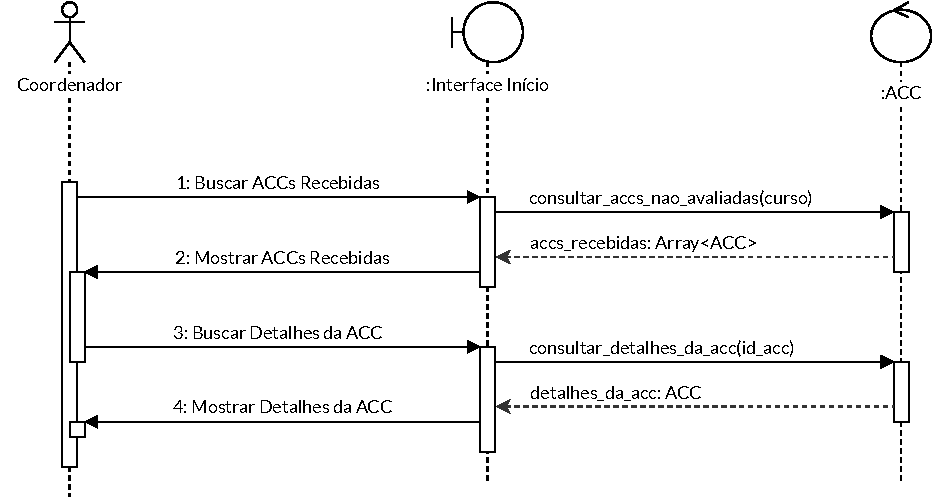
\includegraphics[width=\textwidth]{dados/figuras/Proposta/DiagramasDeSequencia/Consultar ACC.pdf}
    \caption{Diagrama de Sequência: Consultar ACC.}
    \label{diagSeq:coordConsultarACC}
\end{figure}

A Figura \ref{diagSeq:avaliarRequisicaoACC} representa a sequência das ações descritas na Tabela \ref{casoExpandido:avaliarACCs}. Esse fluxo mostra a sequência de eventos que acontecem no sistema ao ser realizada uma avaliação por parte de um Coordenador. O primeiro passo é a busca das ACCs Recebidas, realizada pelo Coordenador através da interface; Após isso o sistema exibe as ACCs recebidas, e o Coordenador escolhe uma das ACCs para buscar os detalhes; O sistema busca essas informações através do controlador de ACCs e retorna ao Coordenador através da interface; O quinto passo é a Avaliação da ACC, a partir dessa avaliação o sistema chama o controlador ACC que por sua vez chama um método para si mesmo para atualizar o \textit{status} da ACC para aprovada ou reprovada, dependendo da avaliação, e salva a avaliação da ACC através do método de salvamento do controlador AvaliacaoDaACC; Por último o sistema exibe ao Coodenador uma mensagem de confirmação de salvamento da avaliação.

\begin{figure}[H]
    \centering
    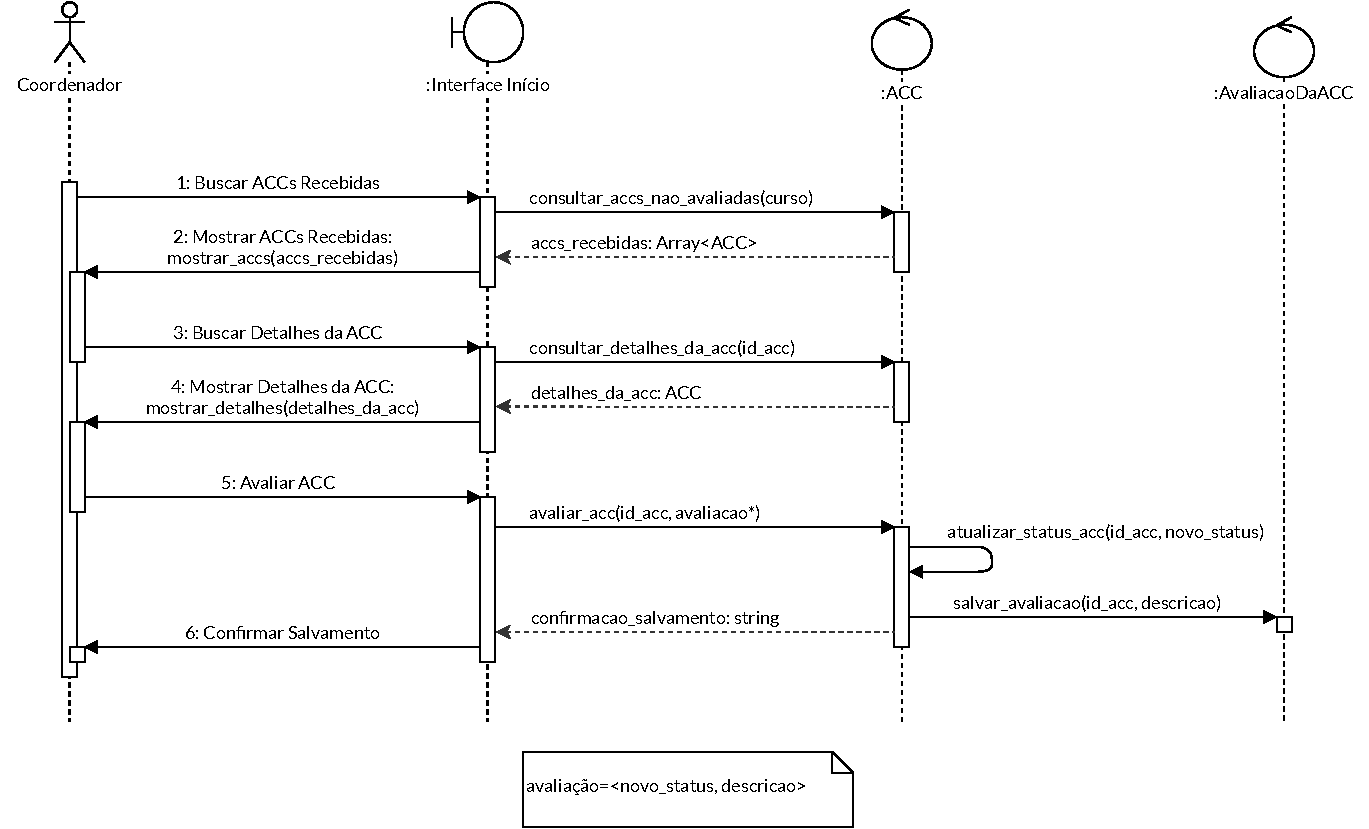
\includegraphics[width=\textwidth]{dados/figuras/Proposta/DiagramasDeSequencia/Avaliar Requisição de ACC.pdf}
    \caption{Diagrama de Sequência: Avaliar ACC.}
    \label{diagSeq:avaliarRequisicaoACC}
\end{figure}

A Figura \ref{diagSeq:consultarDiscente} representa a sequência das ações descritas na Tabela \ref{casoExpandido:consultarDiscentes}, que são realizadas por um Coordenador ao fazer a consulta dos detalhes de um Discente. O Coordenador faz a consulta dos Discentes passando como parâmetro um campo de busca através da tela de Pesquisar Discente; O sistema então faz a consulta dos Discentes através do controlador Usuario e retorna os Discentes encontrados com o parâmetro, e que estão vinculados ao mesmo curso do Coordenador, de volta para a interface, que por sua vez faz a exibição dos Discentes; A partir disso o Coordenador escolhe um dos Discentes, e consulta os seus detalhes; O sistema então faz a busca dos detalhes do Discente usando o controlador Usuario; O controlador retorna os detalhes, que por sua vez são exibidos pela interface ao Coordenador.

\begin{figure}[H]
    \centering
    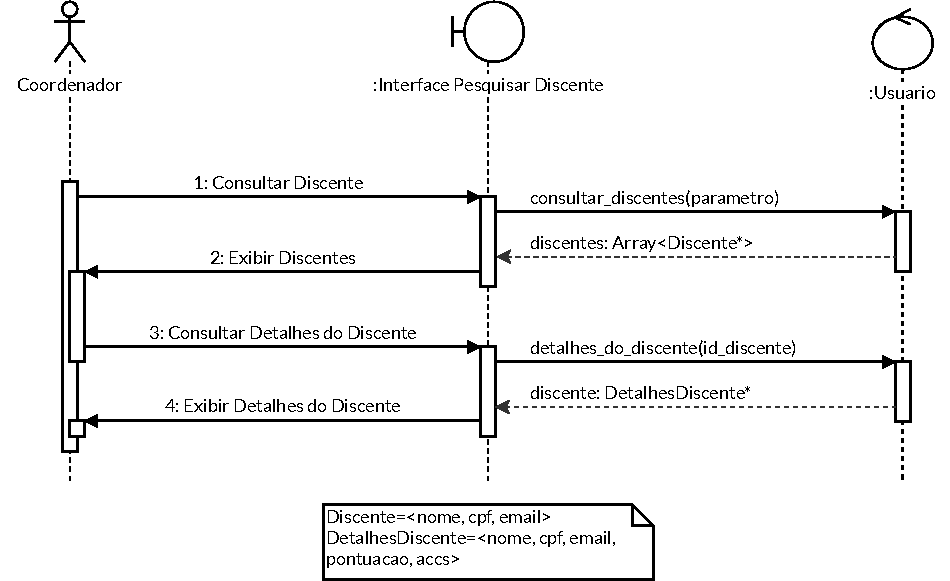
\includegraphics[width=\textwidth]{dados/figuras/Proposta/DiagramasDeSequencia/Consultar Discente.pdf}
    \caption{Diagrama de Sequência: Consultar Discente.}
    \label{diagSeq:consultarDiscente}
\end{figure}

% Discente -------------------------------------

A Figura \ref{diagSeq:consultarPontuacao} representa a sequência das ações descritas na Tabela \ref{casoExpandido:consultarPontuacao}. O diagrama demonstra o fluxo das ações de consulta da pontuação de um Discente. Primeiramente, o Discente busca a sua pontuação através da interface, após isso, o sistema envia o pedido ao controlador ACC, que calcula a pontuação de ACCs através das ACCs do Discente; Após isso o sistema retorna os resultados através da interface, exibindo na tela os pontos aprovados, em análise e reprovados do Discente.

\begin{figure}[H]
    \centering
    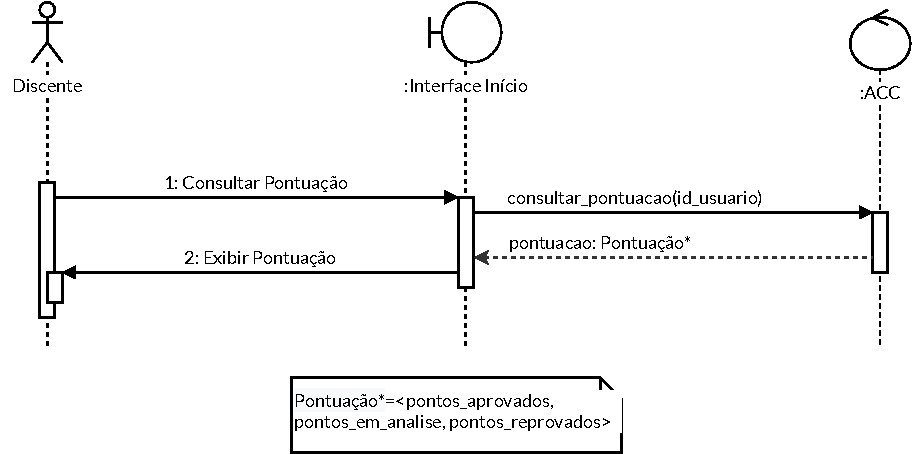
\includegraphics[width=\textwidth]{dados/figuras/Proposta/DiagramasDeSequencia/Consultar Pontuação.pdf}
    \caption{Diagrama de Sequência: Consultar Pontuação.}
    \label{diagSeq:consultarPontuacao}
\end{figure}

A Figura \ref{diagSeq:consultarTiposDeACC} representa a sequência das ações descritas na Tabela \ref{casoExpandido:consultarTiposDeACC}, que está relacionada à ação de um usuário do tipo Discente de consultar os Tipos de ACC presentes no sistema. Primeiramente, o Discente consulta os Tipos de ACC através da interface; Após isso, o sistema envia o pedido ao controlador TiposDeACC; O controlador retorna os Tipos de ACC para a interface, que por sua vez exibe para o Discente.

\begin{figure}[H]
    \centering 
    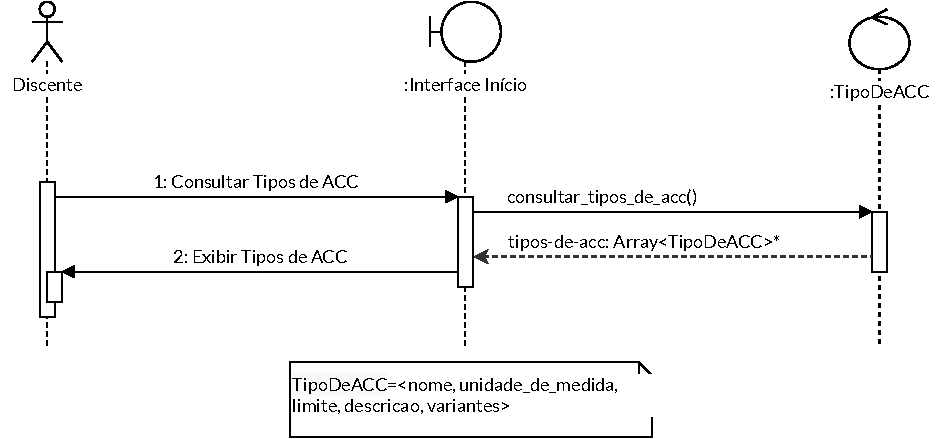
\includegraphics[width=\textwidth]{dados/figuras/Proposta/DiagramasDeSequencia/Consultar Tipos de ACC.pdf}
    \caption{Diagrama de Sequência: Consultar Tipos de ACC}
    \label{diagSeq:consultarTiposDeACC}
\end{figure}


A Figura \ref{diagSeq:gerenciarACCs} representa a sequência das ações descritas na Tabela \ref{casoExpandido:gerenciarACCs}. Esse diagrama sequencial representa as principais ações que um usuário do tipo Discente poderá realizar em relação às ACCs. A primeira etapa que o Discente realizará é a de abrir a Tela de Gerenciamento de ACCs a partir da Tela de Início; O sistema então buscará as ACCs pelo id do Discente e retornará essas ACCs à interface que fará a exibição dos dados; O Discente então escolhe uma ação entre: Cadastrar, Consultar, Editar ou Excluir; 

A partir disso o diagrama foi separado através da notação \textit{opt}, que descreve escolhas dentro de uma sequência. Essas escolhas possuem dentro de si referências, criadas através da notação \textit{ref}. Como pode ser observado na Figura \ref{diagSeq:gerenciarACCs}, há 4 \textit{opts}, sendo que cada um destes possui uma referência à outro diagrama de sequência, sendo estas: opt1 descrita na Figura \ref{diagSeq:cadastrarACC}; opt2, referenciando a Figura \ref{diagSeq:consultarACC}; opt3, como referência para a Figura \ref{diagSeq:editarACC}; e opt4 que se relaciona com a Figura \ref{diagSeq:excluirACC}.

\begin{figure}[H]
    \centering 
    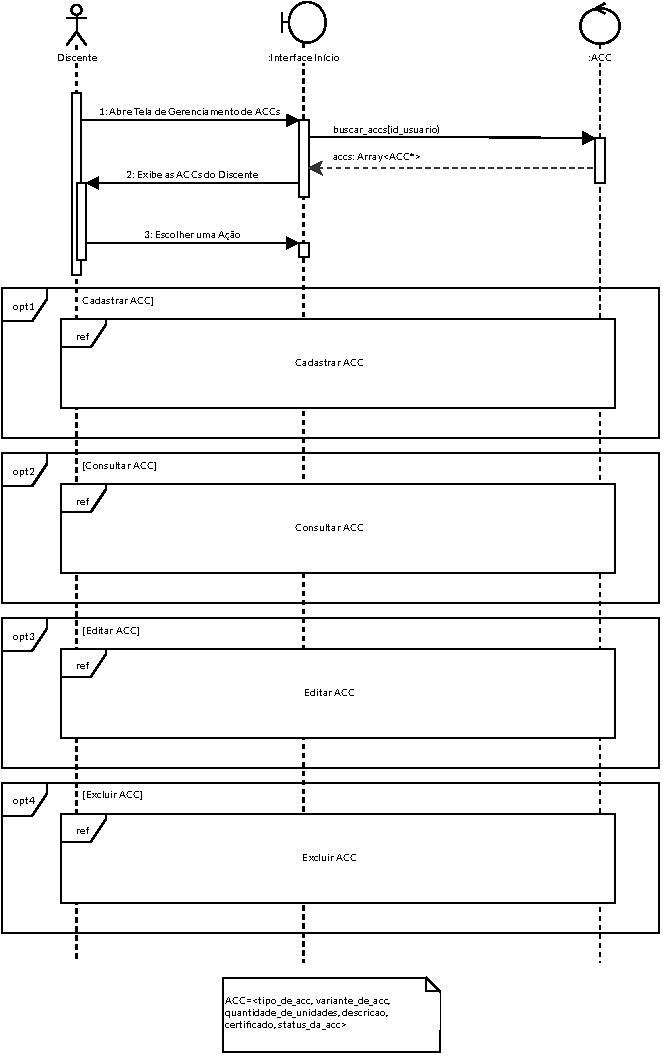
\includegraphics[width=0.8\textwidth]{dados/figuras/Proposta/DiagramasDeSequencia/Gerenciar ACCs_ Completo-Completo.pdf}
    \caption{Diagrama de Sequência: Gerenciar ACCs}
    \label{diagSeq:gerenciarACCs}
\end{figure}

A Figura \ref{diagSeq:cadastrarACC} demonstra a sequência de ações realizadas dentro do caso de uso de Cadastrar uma ACC, realizado por um Discente. Esse ação está presente no diagrama de sequência da Figura \ref{diagSeq:gerenciarACCs}. Conforme mostrado no diagrama, o Discente primeiro cadastra uma nova ACC através da tela de Cadastrar ACC preenchendo os campos necessários; Após isso o sistema faz a chamada o método de cadastro de ACC para o controlador ACC, que por sua vez retorna a confirmação de cadastro; A interface então recebe a mensagem de confirmação de cadastro e faz sua exibição.

\begin{figure}[H]
    \centering 
    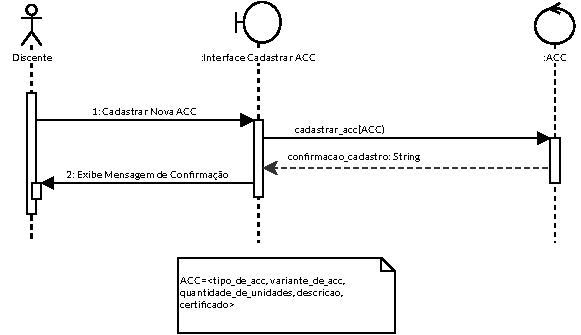
\includegraphics[width=\textwidth]{dados/figuras/Proposta/DiagramasDeSequencia/Gerenciar ACCs_ Completo-Cadastrar ACC.pdf}
    \caption{Diagrama de Sequência: Cadastrar ACC}
    \label{diagSeq:cadastrarACC}
\end{figure}

A Figura \ref{diagSeq:consultarACC} demonstra a sequência de ações realizadas pela ação de Consultar uma ACC, referenciada pelo diagrama de sequência da Figura \ref{diagSeq:gerenciarACCs}. Como mostrado no gráfico, o Discente Busca os detalhes de uma ACC através da tela de Consultar ACC; o sistema então faz a chamada do método de busca dos detalhes da ACC através do id; após isso, são retornados os detalhes da ACC selecionada, que são posteriormente exibidos ao Discente pela interface gráfica.

\begin{figure}[H]
    \centering 
    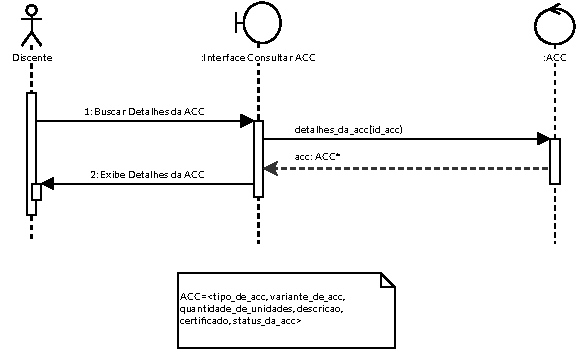
\includegraphics[width=\textwidth]{dados/figuras/Proposta/DiagramasDeSequencia/Gerenciar ACCs_ Completo-Consultar ACC.pdf}
    \caption{Diagrama de Sequência: Consultar ACC}
    \label{diagSeq:consultarACC}
\end{figure}

A Figura \ref{diagSeq:editarACC} mostra o diagrama de sequência relativo à Edição de uma ACC. Esse fluxo é referenciado pelo diagrama de sequência da Figura \ref{diagSeq:gerenciarACCs}. Como é mostrado na figura, o Discente primeiramente busca os detalhes da ACC desejada; O sistema então faz a busca pelo controlador de ACC, e retorna a ACC encontrada à interface que faz a exibição dos dados; O Discente então faz a edição dos campos através da tela de Editar ACC e envia suas alterações; O sistema por sua vez, encaminha essas alterações ao controlador, que faz o salvamento dessas edições e retorna uma mensagem de confirmação; o sistema então exibe uma mensagem de confirmação de edição ao Discente.

\begin{figure}[H]
    \centering 
    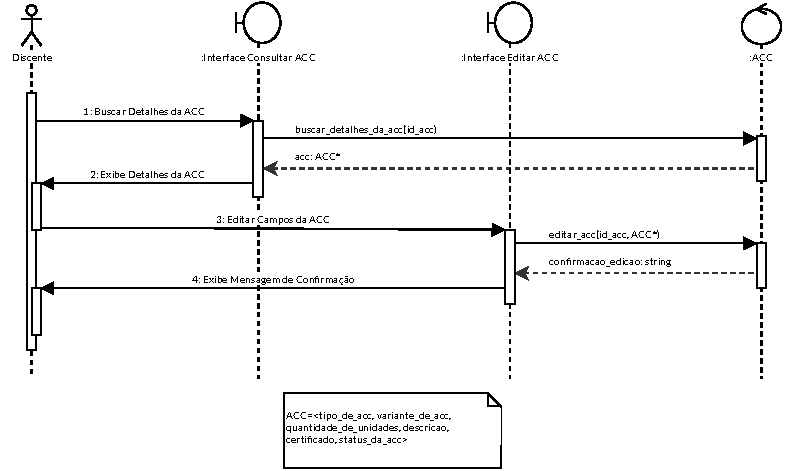
\includegraphics[width=\textwidth]{dados/figuras/Proposta/DiagramasDeSequencia/Gerenciar ACCs_ Completo-Editar ACC.pdf}
    \caption{Diagrama de Sequência: Editar ACC}
    \label{diagSeq:editarACC}
\end{figure}

A Figura \ref{diagSeq:excluirACC} mostra o diagrama de sequência relativo à Exclusão de uma ACC. Esse fluxo é referenciado pelo diagrama de sequência da Figura \ref{diagSeq:gerenciarACCs}. Como é mostrado na figura, o Discente primeiramente busca os detalhes da ACC desejada; O sistema então faz a busca pelo controlador de ACC, e retorna a ACC encontrada à interface que faz a exibição dos dados; O Discente então escolhe a opção de Excluir ACC através da tela de Consultar ACC; Após isso, o sistema faz a chamada da função de Excluir ACC do controlador de ACC; o controlador então envia uma mensagem de confirmação de exclusão, que por sua vez é mostrada ao Discente através da interface.

\begin{figure}[H]
    \centering 
    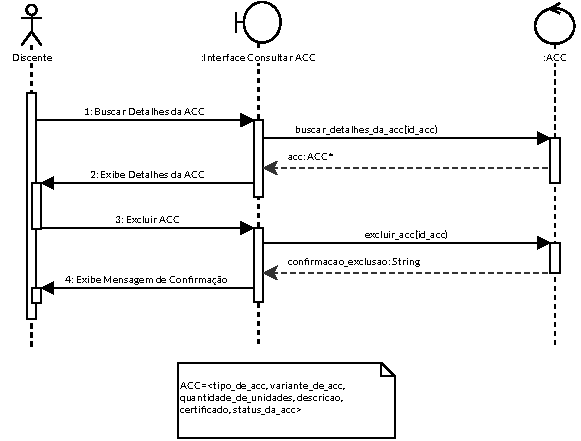
\includegraphics[width=\textwidth]{dados/figuras/Proposta/DiagramasDeSequencia/Gerenciar ACCs_ Completo-Excluir ACC.pdf}
    \caption{Diagrama de Sequência: Excluir ACC}
    \label{diagSeq:excluirACC}
\end{figure}

% Administrador -------------------------------------

O diagrama de sequência mostrado na Figura \ref{diagSeq:gerenciarTiposDeACC} diz respeito ao caso de uso expandido descrito na Tabela \ref{casoExpandido:gerenciarTiposDeACC}. Essa sequência descreve as ações de Cadastro, Atualização, Consulta e Exclusão dos Tipos de ACC presentes no sistema e que podem ser realizadas por um usuário do tipo Administrador. O Administrador primeiramente abre a tela de Gerenciamento de Tipos de ACC através da tela de Início; O sistema então faz a chamada do método de busca dos Tipos de ACC presentes no sistema através do controlador TipoDeACC; O sistema então retorna esses dados à interface que por sua vez exibe ao Administrador; O Administrador então escolhe uma das ações entre: Cadastrar, Consultar, Editar ou Excluir; A partir disso, o sistema redireciona o Administrador para as a tela da ação escolhida. Como pode ser visto na Figura \ref{diagSeq:gerenciarTiposDeACC} as ações foram divididas através de notações \textit{opt}, que por sua vez contém as referências das ações. A opt1 refere-se ao diagrama presente na Figura \ref{diagSeq:cadastrarTipoDeACC}; Já a opt2 referencia a Figura \ref{diagSeq:consultarTipoDeACC}; A opt3 por sua vez faz referência à Figura \ref{diagSeq:editarTipoDeACC}; E por último a opt4 está ligada à Figura \ref{diagSeq:excluirTipoDeACC}.

\begin{figure}[H]
    \centering
    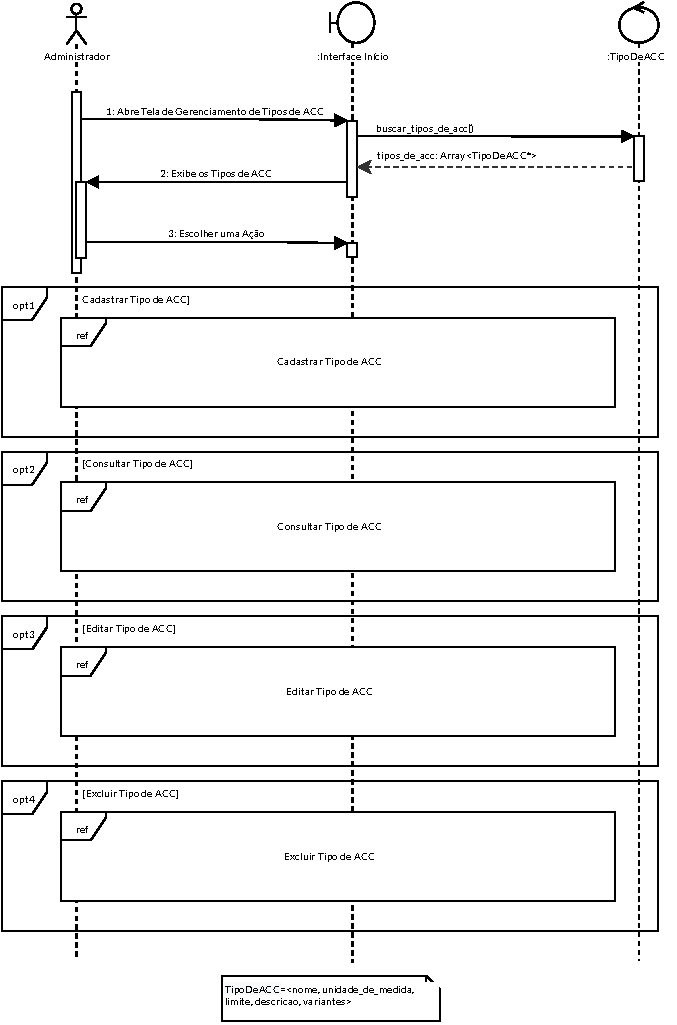
\includegraphics[width=0.8\textwidth]{dados/figuras/Proposta/DiagramasDeSequencia/Gerenciar Tipos de ACC-Completo.pdf}
    \caption{Diagrama de Sequência: Gerenciar Tipos de ACC}
    \label{diagSeq:gerenciarTiposDeACC}
\end{figure}

A Figura \ref{diagSeq:cadastrarTipoDeACC} engloba a sequência de eventos que acontecem no cadastro de um Tipo de ACC, o diagrama refere-se a uma das ações contidas dentro da Figura \ref{diagSeq:gerenciarTiposDeACC}. O Administrador do sistema faz o cadastro do Tipo de ACC preenchendo os campos necessários através da tela de Cadastrar Tipo de ACC; A interface por sua vez faz a chamada do método de cadastro de Tipo de ACC através do controlador TipoDeACC; Após isso, o controlador envia uma mensagem de confirmação de cadastro à interface, que por sua vez à exibe ao Administrador.

\begin{figure}[H]
    \centering
    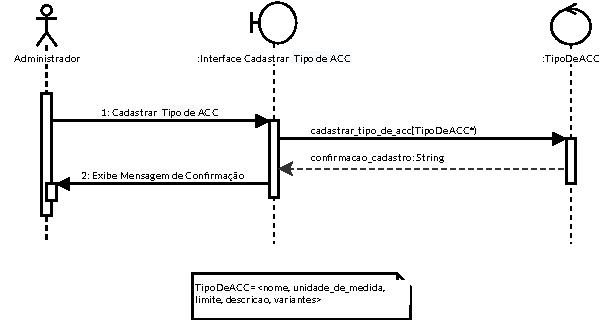
\includegraphics[width=\textwidth]{dados/figuras/Proposta/DiagramasDeSequencia/Gerenciar Tipos de ACC-Cadastrar Tipo de ACC.pdf}
    \caption{Diagrama de Sequência: Cadastrar Tipo de ACC}
    \label{diagSeq:cadastrarTipoDeACC}
\end{figure}

O diagrama descrito na Figura \ref{diagSeq:consultarTipoDeACC} é uma referência à ação de Consultar Tipo de ACC, presente no diagrama mostrado na Figura \ref{diagSeq:gerenciarTiposDeACC}. O consultor primeiramente realiza a busca dos detalhes de um Tipo de ACC, através da interface gráfica; O sistema por sua vez faz a chamada do método que faz a consulta dos detalhes de um Tipo de ACC; A partir disso, o controlador retorna esses dados à interface que por sua vez faz a exibição ao Administrador.

\begin{figure}[H]
    \centering
    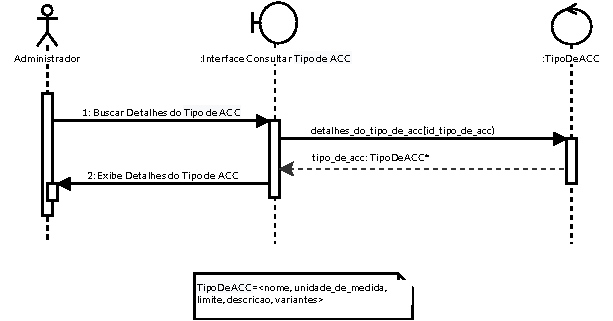
\includegraphics[width=\textwidth]{dados/figuras/Proposta/DiagramasDeSequencia/Gerenciar Tipos de ACC-Consultar Tipo de ACC.pdf}
    \caption{Diagrama de Sequência: Consultar Tipo de ACC}
    \label{diagSeq:consultarTipoDeACC}
\end{figure}

A ação de Editar Tipo de ACC, presente no diagrama da Figura \ref{diagSeq:gerenciarTiposDeACC} está descrito na Figura \ref{diagSeq:editarTipoDeACC}. O Administrador primeiramente faz a consulta dos detalhes do Tipo de ACC através da tela de Consultar Tipo de ACC; O sistema por sua vez chama a função de buscar detalhes do Tipo de ACC presente no controlador TipoDeACC; O controlador por sua vez, retorna os dados do Tipo de ACC que são então retornados ao Administrador através da interface gráfica; O Administrador então faz o preenchimento das alterações necessárias no Tipo de ACC através da tela de Editar Tipo de ACC e submete essas alterações; A interface envia essas alterações para serem salvas pelo controlador; O controlador então retorna uma mensagem de confirmação da edição, que por sua vez é exibida ao Administrador através da interface.

\begin{figure}[H]
    \centering
    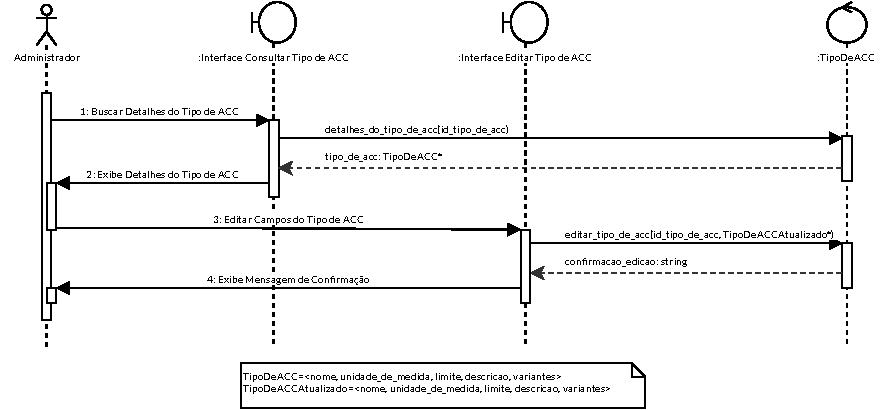
\includegraphics[width=\textwidth]{dados/figuras/Proposta/DiagramasDeSequencia/Gerenciar Tipos de ACC-Atualizar Coordenador.pdf}
    \caption{Diagrama de Sequência: Editar Tipo de ACC}
    \label{diagSeq:editarTipoDeACC}
\end{figure}

A Figura \ref{diagSeq:excluirTipoDeACC} demonstra o diagrama de sequência correspondente à ação de Excluir Tipo de ACC, presente no diagrama encontrado na Figura \ref{diagSeq:gerenciarTiposDeACC}, e descreve a sequência de eventos que acontecem durante a exclusão de um Tipo de ACC realizada por um Administrador. O Administrador faz a busca dos Detalhes do Tipo de ACC através da interface, esta faz a chamada do método de consulta dos detalhes de um Tipo de ACC presente no controlador TipoDeACC; O controlador retorna os dados do Tipo de ACC à interface que por sua vez exibe ao Administrador; O Administrador então escolhe a opção de Excluir Tipo de ACC; A partiri disso, o sistema faz a exclusão do Tipo de ACC utilizando o identificador único do Tipo de ACC; O controlador então envia uma mensagem de confirmação da exclusão, que é então exibida ao Administrador pela interface.

\begin{figure}[H]
    \centering
    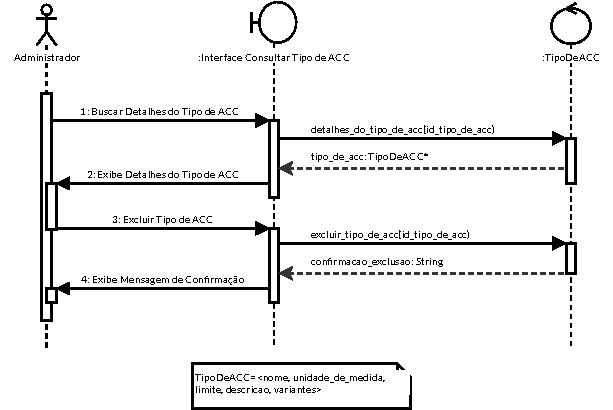
\includegraphics[width=\textwidth]{dados/figuras/Proposta/DiagramasDeSequencia/Gerenciar Tipos de ACC-Excluir Tipo de ACC.pdf}
    \caption{Diagrama de Sequência: Excluir Tipo de ACC}
    \label{diagSeq:excluirTipoDeACC}
\end{figure}

O diagrama de sequência mostrado na Figura \ref{diagSeq:gerenciarCoordenadores} diz respeito ao caso de uso expandido descrito na Tabela \ref{casoExpandido:gerenciarCoordenadores}, e mostra o gerenciamento de coordenadores, ação realizada por um usuário do tipo Administrador. Conforme o diagrama, a primeira ação que o Administrador realiza é a de abrir a tela de gerenciamento de Coordenadores através da tela Inicial; Após isso, o sistema busca os usuários do tipo Coordenador presentes no sistema através do controlador Usuario; Após isso, o controlador retorna os Coordenadores encontrados à interface que por sua vez renderiza a lista recebida; O Administrador então escolhe uma ação entre: Cadastrar, Consultar, Editar e Excluir. Como pode ser visto na Figura \ref{diagSeq:gerenciarCoordenadores}, essas ações são divididas utilizando a notação \textit{opt}, que denota opções que podem ser escolhidas dentro de uma sequência, cada uma dessas \textit{opts} possuem uma referência para outro diagrama de sequência utilizando a notação \textit{ref}, tal estratégia foi utilizada para diminuir a complexidade do diagrama e melhorar a compreensão. As ações estão referenciadas da seguinte forma: opt1 fazendo referência à Figura \ref{diagSeq:cadastrarCoordenador}; opt2 sendo demonstrada na Figura \ref{diagSeq:consultarCoordenador}; opt3 referenciando a Figura \ref{diagSeq:editarCoordenador}; e opt4 sendo uma referência à Figura \ref{diagSeq:excluirCoordenador}.

\begin{figure}[H]
    \centering
    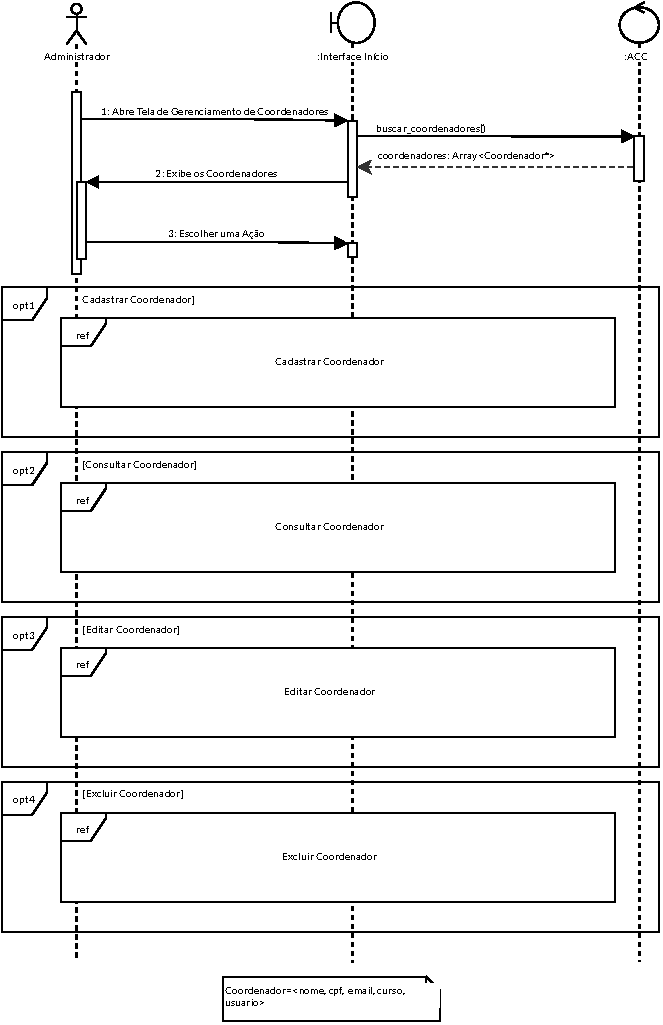
\includegraphics[width=0.8\textwidth]{dados/figuras/Proposta/DiagramasDeSequencia/Gerenciar Coodenadores-Completo}
    \caption{Diagrama de Sequência: Gerenciar Coordenadores}
    \label{diagSeq:gerenciarCoordenadores}
\end{figure}

A Figura \ref{diagSeq:cadastrarCoordenador} demonstra o diagrama de sequência referente ao cadastro de um Coordenador, presente dentro do diagrama de Gerenciamento de Coordenadores, mostrado na Figura \ref{diagSeq:gerenciarCoordenadores}. O Administrador primeiramente realiza o cadastro de um Coordenador através da tela de Cadastrar Coordenador; A interface então faz a chamada do método de cadastrar um novo usuário do tipo coordenador através do controlador Usuario; O controlador então retorna uma mensagem de confirmação de cadastro que por sua vez é exibida ao usuário através da interface.

\begin{figure}[H]
    \centering
    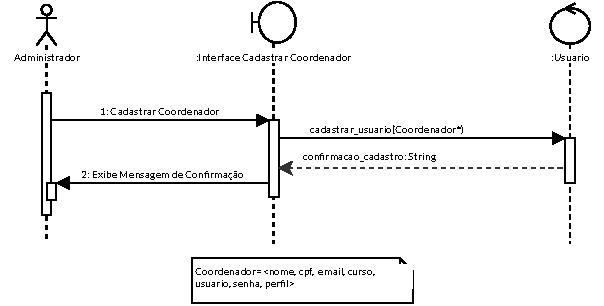
\includegraphics[width=\textwidth]{dados/figuras/Proposta/DiagramasDeSequencia/Gerenciar Coodenadores-Cadastrar Coordenador.pdf}
    \caption{Diagrama de Sequência: Cadastrar Coordenador}
    \label{diagSeq:cadastrarCoordenador}
\end{figure}

A Figura \ref{diagSeq:consultarCoordenador} mostra o diagrama de sequência referente à ação de Consultar Coordenador, presente na Figura \ref{diagSeq:gerenciarCoordenadores}, e demonstra a sequência de eventos que acontecem quando um Administrador realiza a consulta dos detalhes de um Coordenador. O Administrador escolhe um dos Coordenadores e busca os seus detalhes; A interface busca os detalhes do Coordenador através do método de consulta presente no controlador de Usuario; Após isso, o controlador retorna os dados do Coordenador à interface, que por sua vez exibe ao Administrador.

\begin{figure}[H]
    \centering
    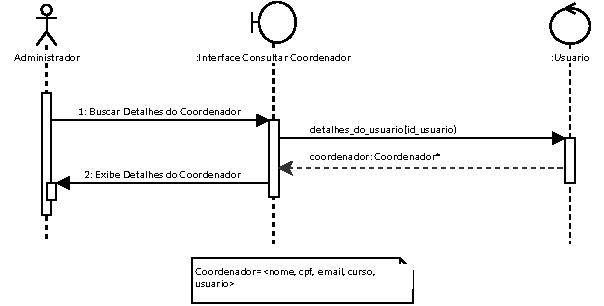
\includegraphics[width=\textwidth]{dados/figuras/Proposta/DiagramasDeSequencia/Gerenciar Coodenadores-Consultar Coordenador.pdf}
    \caption{Diagrama de Sequência: Consultar Coordenador}
    \label{diagSeq:consultarCoordenador}
\end{figure}

A Figura \ref{diagSeq:editarCoordenador} mostra o diagrama de sequência de Editar Coordenador, ação realizada por um Administrador e presente dentro do diagrama de sequência da Figura \ref{diagSeq:gerenciarCoordenadores}. A primeira ação realizada pelo Administrador é fazer a busca dos detalhes de um Coordenador através da Tela de Consultar Coordenador; O sistema faz a busca desses detalhes através do método presente no controlador de Usuario; O controlador retorna os detalhes do Discente à interface, que por sua vez exibe ao Administrador; A partir disso, o Administrador escolhe a opção de Editar Coordenador, e faz a edição dos detalhes do Coordenador através da tela de Editar Coordenador; O Administrador então submete as alterações, que são enviadas ao controlador pela interface; O controlador faz o salvamento dos dados e retorna uma mensagem de confirmação da edição que por sua vez é exibida ao Administrador pela interface gráfica.

\begin{figure}[H]
    \centering
    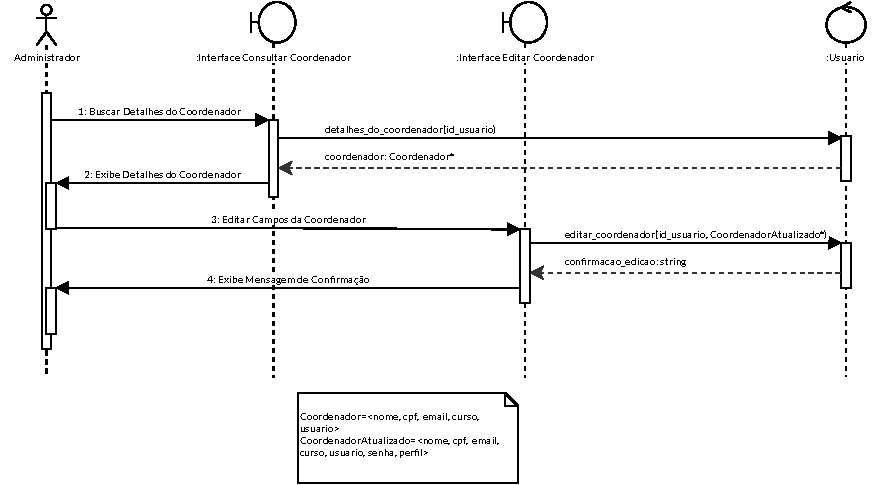
\includegraphics[width=\textwidth]{dados/figuras/Proposta/DiagramasDeSequencia/Gerenciar Coodenadores-Atualizar Coordenador.pdf}
    \caption{Diagrama de Sequência: Editar Coordenador}
    \label{diagSeq:editarCoordenador}
\end{figure}

A Figura \ref{diagSeq:excluirCoordenador} exibe o diagrama de sequência referente à ação de Excluir Coordenador, presente no diagrama de sequência exibido na Figura \ref{diagSeq:gerenciarCoordenadores}. O Administrador faz a busca dos detalhes do Coordenador, através da tela de Consultar Coordenador; O sistema faz a busca dos dados através do controlador de Usuario; O controlador então retorna os dados que são então exibidos ao Administrador através da interface gráfica; Após isso o Administrador seleciona a opção de Excluir Coordenador; O sistema realiza a exclusão do Coordenador utilizando o seu identificador único através do método presente no controlador Usuario; O controlador então retorna uma mensagem de confirmação da exclusão, que é então exibida ao Administrador através da interface gráfica.

\begin{figure}[H]
    \centering
    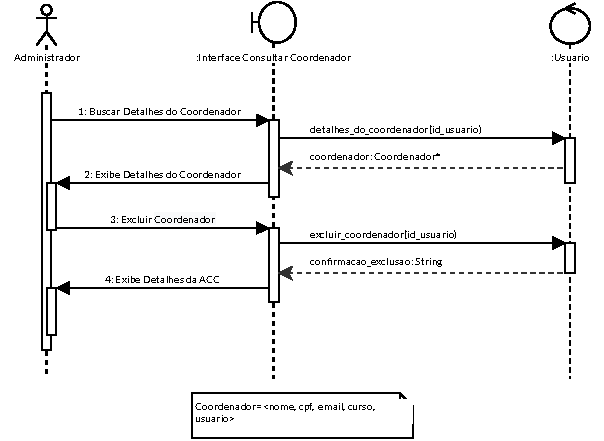
\includegraphics[width=\textwidth]{dados/figuras/Proposta/DiagramasDeSequencia/Gerenciar Coodenadores-Excluir Coordenador.pdf}
    \caption{Diagrama de Sequência: Excluir Coordenador}
    \label{diagSeq:excluirCoordenador}
\end{figure}

\subsection{Modelo Conceitual}
\label{sec:modeloConceitual}

Segundo \cite{wazlawick2014analise} o modelo conceitual descreve a informação que será gerenciada pelo sistema, mostrando uma visão de próxima à de um usuário do sistema. A Figura \ref{fig:modeloConceitual} descreve as informações manipuladas pelo sistema, sendo estas:
\begin{itemize}
    \item Curso: descreve o curso ao qual um usuário está vinculado, sendo necessário apenas o nome do mesmo. Ele se relaciona diretamente com a entidade Usuario através de uma relação de Um para Muitos, onde um curso pode possuir vários usuários, mas cada usuário pode possuir apenas um curso;
    \item Usuario: é a informação sobre o usuário que está utilizando o sistema, sendo responsável por guardar tanto os dados dos discentes, quanto dos coordenadores e administradores. Essa entidade está ligada à Enumeração Perfil, que por sua vez descreve qual o perfil do usuário cadastrado, através de uma relação de Muitos para Um, onde cada Perfil possui vários Usuarios, mas cada Usuario possui apenas um Perfil; A mesma relação de Usuario e Perfil é encontrada entre Usuario e Curso; Há ainda uma relação de Um para Muitos com a entidade ACC, e de Um para Um com Login, onde cada Usuario possui um Login e vice-versa;
    \item Login: responsável por guardar os dados de login de um usuário, bem como o seu token de acesso ao sistema. Essa informação relaciona-se de Um para Um com o Usuario, pois cada Usuario possui apenas um Login, e um Login apenas um Usuario;
    \item ACC: guarda as informações sobre a ACC de um discente. Está ligada à Enumeração StatusDaACC, que mostra qual o estado da ACC dentro do sistema (Aprovada, Reprovada ou Em análise), através de uma relação de Muitos para Um, a mesma relação se encontra com as entidades Usuario, TipoDeACC e VarianteDaACC; Já o relacionamento de ACC com Certificado é de Um para Um, onde cada ACC possui apenas um Certificado e vice-versa;
    \item Certificado: responsável por guardar os dados de um certificado vinculado a uma ACC. Relaciona-se unicamente com ACC, numa relação de Um para Um;
    \item TipoDeAcc: guarda os tipos de ACC presentes no sistema, sendo necessária a utilização da Enumeração UnidadeDeMedida, que descreve os tipos de unidade de medida do sistema (Hora, Semestre, Curso etc). Possui uma relação de Um para Muitos com ACC, onde cada TipoDeACC pode ter várias ACCs, mas cada ACC pode possuir apenas um TipoDeACC; Já sua relação com VarianteDaACC se dá em Um para Um, e com UnidadeDeMedida em Muitos para Um;
    \item VarianteDeAcc: guarda os tipos de variações de ACCs, por exemplo se uma ACC é na área dos cursos da FACEEL ou não. As variações são utilizadas para o calculo de proporção por unidade de medida do tipo de ACC que ela está associada. Relaciona-se de Um para Muitos com ACC, e de Um para Um com TipoDeACC;
    \item UnidadeDeMedida: Responsável por guardar as unidades de medida presentes nos TiposDeACC, essas unidades são Hora, Semestre, Curso, Trabalho, entre outros. Possui relação unicamente com TipoDeACC, em uma proporção de Um para Muitos;
\end{itemize}

\begin{figure}[H]
    \centering
    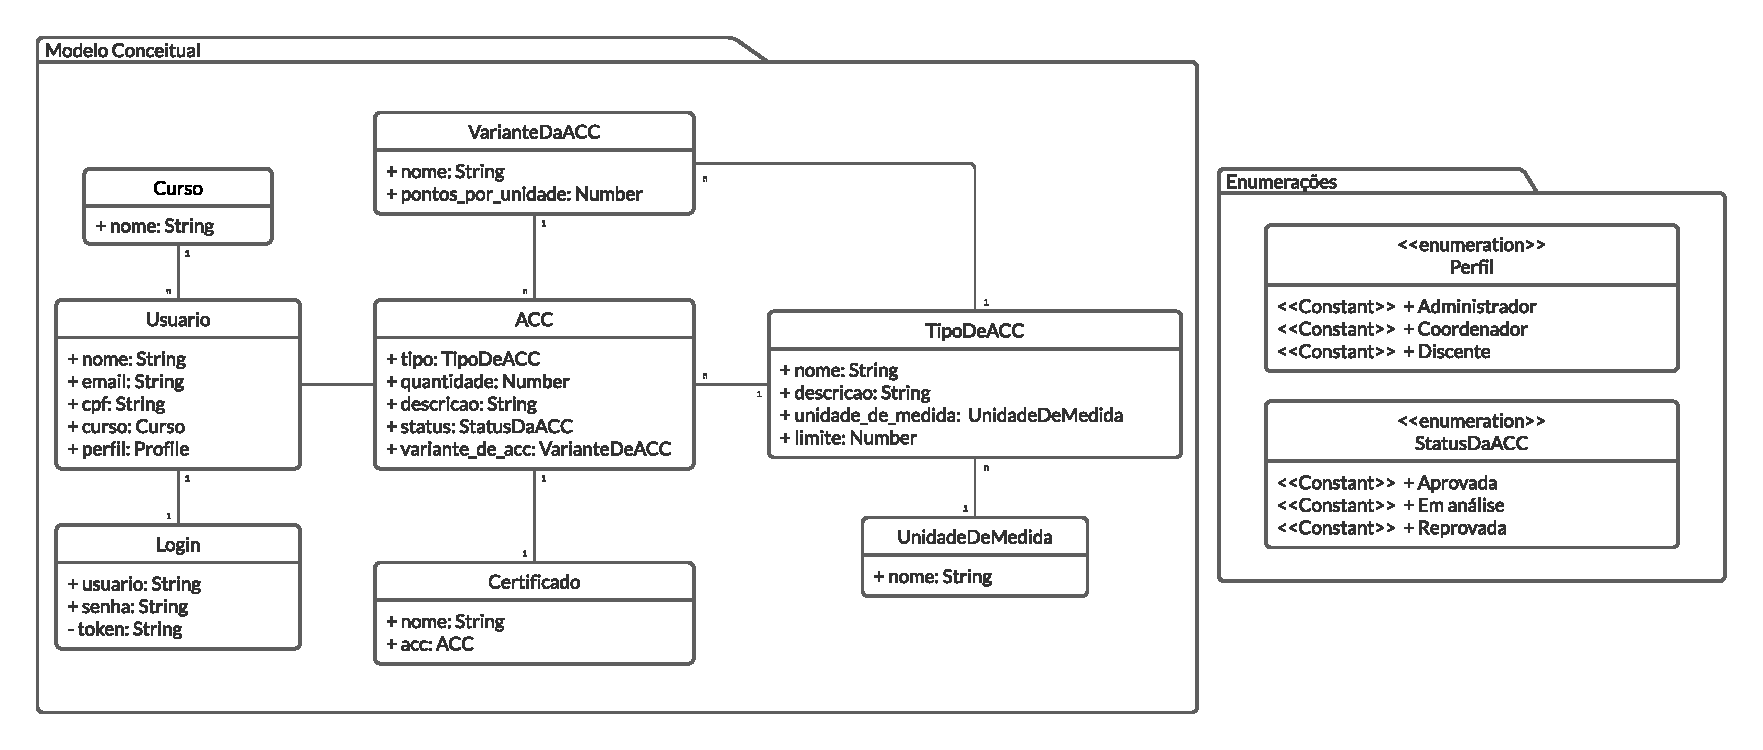
\includegraphics[width=\textwidth]{dados/figuras/Proposta/modelo_conceitual__keeme.pdf}
    \caption{Modelo Conceitual do Sistema}
    \label{fig:modeloConceitual}
\end{figure}

\subsection{Diagrama de Entidade Relacionamento}
\label{sec:diagramaER}

O Diagrama de Entidade Relacionamento, é descrito por \cite{lucid2021er} como sendo um diagrama que mostra como as entidades relacionam-se entre si dentro de um determinado sistema. São utilizados dentro da Engenharia de Software para se fazer a modelagem dos bancos de dados relacionais. A Figura \ref{fig:entidadeRelacionamento} demonstra o diagrama de entidade relacionamento referente à base de dados utilizada pela aplicação desenvolvida neste trabalho.

\begin{figure}[H]
    \centering
    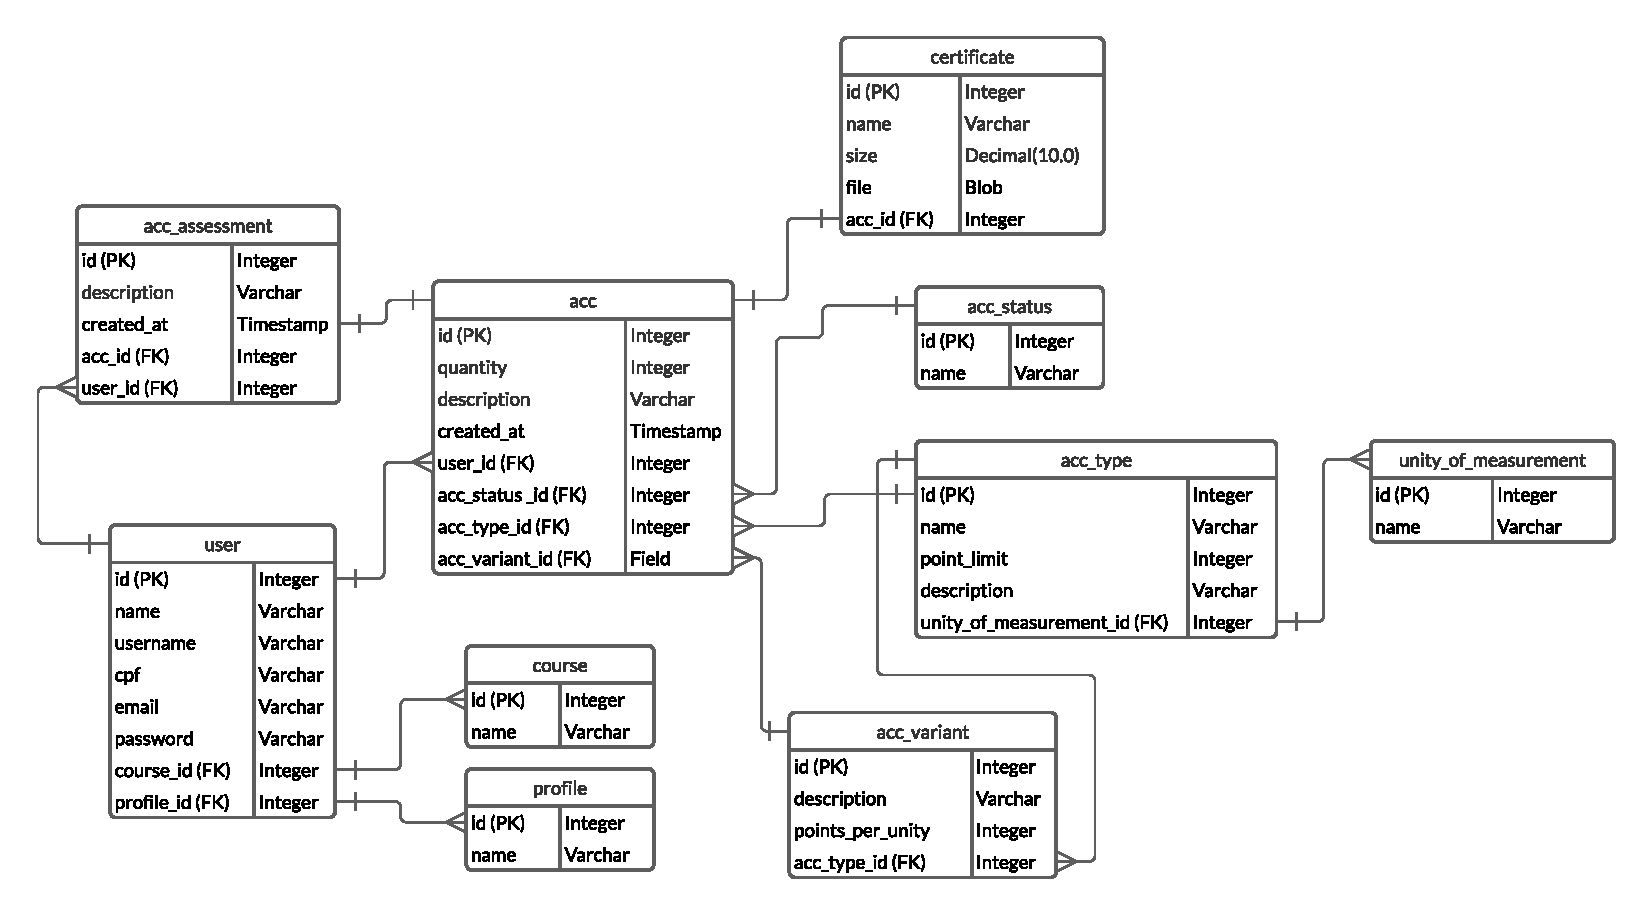
\includegraphics[width=\textwidth]{dados/figuras/Proposta/Diagrama Keep It To Me - v1.0 MVP.pdf}
    \caption{Banco de Dados da Aplicação KeeMe}
    \label{fig:entidadeRelacionamento}
\end{figure}

\begin{itemize}
    
    \item user (usuário): essa entidade armazena os dados dos usuários da aplicação. Seus campos são:
    \begin{itemize}
        \item id: identificador único do usuário;
        \item name (nome): guarda o nome do usuário;
        \item username: guarda o apelido do usuário, utilizado para a função de login na plataforma;
        \item cpf: armazena o cpf do usuário, utilizado para facilitar as funções de busca de discentes;
        \item email: campo referente ao email do usuário, utilizado para funções que envolvam confirmação de criação de perfil e recuperação de senhas;
        \item password (senha): senha que o usuário utilizará para entrar no sistema. Nesta aplicação em específico, está sendo usada a criptografia MD5 para armazenar as senhas dos usuários, e impedir a sua desencriptação;
        \item course\_id: id do curso ao qual o usuário está vinculado. Um usuário pode estar vinculado a apenas um curso;
        \item profile\_id: id do perfil do usuário no sistema. Um usuário pode ter apenas um perfil por vez;
    \end{itemize}
    
    \item course (curso): entidade responsável por armazenar os dados dos cursos presentes na base. Um curso pode ter um ou mais usuários, porém um usuário pode ter apenas um curso. Seus campos são:
    \begin{itemize}
        \item id: identificador único do curso;
        \item name (nome): nome do curso;
    \end{itemize}
    
    \item profile (perfil): responsável por guardar os perfis dos usuários no sistema, é utilizada para funções de autenticação de usuários. Um perfil pode conter um ou mais usuários, mas cada usuário pode ter apenas um perfil no sistema. Seus campos são:
    \begin{itemize}
        \item id: identificador único do perfil;
        \item name (nome): nome do perfil;
    \end{itemize}
    
    \item unity\_of\_measurement (unidade de medida): Armazena os tipos de unidade de medida presentes no sistema, esses tipos se referem a como os pontos de ACCs são contados, por exemplo: horas, semestres, certificados, etc. Seus campos são:
    \begin{itemize}
        \item id: identificador único da unidade de medida;
        \item name (nome): nome da unidade de medida;
    \end{itemize}
    
    \item acc\_type (tipo de acc): Essa entidade é responsável por guardar os dados de tipos de ACC presentes no sistema, esses tipos são as atividades presentes no regulamento de ACC, como por exemplo a realização de minicursos. Seus campos são:
    \begin{itemize}
        \item id: identificador único do tipo de ACC;
        \item name (nome): nome do tipo de ACC;
        \item point\_limit (limite de pontos): refere-se ao limite máximo de pontos que um usuário pode conseguir em determinada modalidade de ACC;
        \item description (descrição): guarda o detalhamento daquilo que a ACC se refere, sendo um campo adicional para facilitar o entendimento por parte dos discentes;
        \item unity\_of\_measurement\_id: identificador da unidade de medida do tipo de ACC.
    \end{itemize}
    
    \item acc\_variant (variante da acc): esta classe guarda as variantes de ACC presentes no sistema. Variantes são subtipos de ACCs, elas foram criadas por conta da existência de tipos de ACC que possuem mais de um tipo de estratégia de pontuação, mas que essas estratégias estão sob o mesmo limite de pontuação. Seus campos são:
    \begin{itemize}
        \item id: identificador único da variante de acc;
        \item description (descrição): uma descrição do que a variante se refere, por exemplo, minicurso na área dos cursos da FACEEL;
        \item points\_per\_unity (pontos por unidade): esse campo refere-se à quantidade de pontos que um usuário pode obter por unidade de medida do tipo de ACC. Por exemplo, um discente poderá obter 6 pontos por semestre em um estágio não obrigatório, onde os pontos por unidade nesse caso são 6, e a unidade de medida é Semestre;
        \item acc\_type\_id: tipo de ACC ao qual a variante está associada;
    \end{itemize}
    
    \item acc\_status (status da acc): refere-se aos status que as accs estão dentro do sistema, são status como aprovada ou reprovada. Seus campos são:
    \begin{itemize}
        \item id: identificador único do status da ACC;
        \item quantity (nome): nome do status da ACC;
    \end{itemize}

    \item acc: é a classe central do sistema, responsável por guardar as informações sobre as ACCs obtidas pelos discentes do sistema. Seus campos são:
    \begin{itemize}
        \item id: identificador único da ACC;
        \item quantity (quantidade): a quantidade refere-se diretamente à unidade de medida do tipo de ACC ao qual a ACC está associada. Sendo que essa quantidade é o número de horas, semestres, certificados, etc, que o usuário possui naquela ACC;
        \item created\_at (criada em): guarda o momento da criação da ACC;
        \item user\_id (id do usuário): associa a ACC a um usuário presente no sistema;
        \item acc\_status\_id (status da acc): armazena o status da ACC através de uma chave estrangeira;
        \item acc\_type (tipo de acc): referencia o tipo da ACC;
        \item acc\_variant\_id (id da variante de acc): relaciona a ACC a uma variante do sistema;
    \end{itemize}
    
    \item acc\_assessment (avaliação da acc): salva as informações de uma avaliação de ACC realizada por um Coordenador do sistema. Seus campos são:
    \begin{itemize}
        \item id: identificador único da avaliação de ACC;
        \item created\_at (criada em): data da avaliação de ACC;
        \item description (descrição): Motivo pelo qual uma ACC foi reprovada, esse campo só é usado em caso de reprovações;
        \item user\_id (id do usuário): relaciona o coordenador responsável pela avaliação da ACC;
    \end{itemize}
\end{itemize}

\section{Arquitetura do Sistema KeeMe}
\label{sec:arquiteturaDoSistema}

Foi utilizada uma arquitetura baseada em microserviços na aplicação, onde há um servidor \textit{Back-end} que é responsável pela lógica da aplicação, e pelas regras de negócio, e um servidor \textit{Front-end}, cujo intuito e a visualização dos dados e interação com a ferramenta.

A Figura \ref{fig:arquiteturaKeeme} demonstra de maneira visual a arquitetura utilizada na ferramenta KeeMe. O servidor \textit{Back-end} da aplicação é responsável por toda parte lógica da aplicação, como a calculo de pontos dos alunos, e por todas as funções de manipulação da base de dados, sendo que a utilização de suas funções são feitas através dos serviços que ele provê, que são chamados através das rotas providas pelo mesmo. O servidor \textit{Front-end} tem como única responsabilidade prover uma interface de utilização do sistema, desta forma, não possui nenhuma regra de negócio, mas apenas consome os serviços providos pelo \textit{Back-end}, em outras palavras, o \textit{Front-end} não faz nenhuma interação direta com a base de dados. Os clientes por sua vez consomem o \textit{Front-end} através de computadores, celulares ou tablets, e interagem com o sistema através dele, dessa forma os clientes não podem interagir diretamente com o \textit{Back-end} ou com a base, mas apenas com o \textit{Front-end}

\begin{figure}[H]
    \centering
    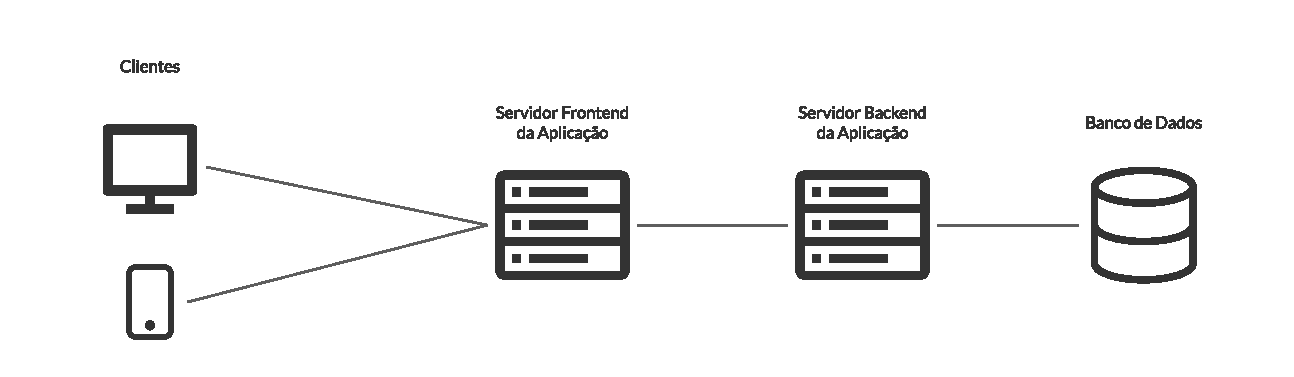
\includegraphics[width=\textwidth]{dados/figuras/Proposta/arquitetura_keeme.pdf}
    \caption{Arquitetura do Sistema KeeMe.}
    \label{fig:arquiteturaKeeme}
\end{figure}

A estratégia de dividir as responsabilidades em microserviços foi utilizada primeiramente pela melhoria na manutenibilidade do sistema, separando a parte visual da parte lógica, e também como forma de desacoplar a lógica do sistema, tornando-a independente, e assim caso haja a necessidade de se refazer o \textit{Front-end}, ou mesmo de criar uma aplicação voltada para dispositivos móveis ou computadores, não é necessário reimplementar a lógica, mas apenas consumir os serviços já providos pelo \textit{Back-end}.

\section{Implementação do KeeMe}
\label{sec:implementacao}

A implementação da aplicação foi feita utilizando o Typescript tanto no \textit{Back-end} quanto no \textit{Front-end}, que por sua vez foi feito utilizando como base a biblioteca React. O desenvolvimento da interface foi feito buscando uma solução que fosse amigável, minimalista, mas que possuísse todas as informações relevantes aos discentes.

\subsection{\textit{Back-end}}

O \textit{Back-end} da aplicação foi criado utilizando o Typescript, implementando um servidor REST, que segundo \cite{costa2020__rest} deve ser visto como um modelo de comunicação entre sistemas distribuídos, no qual o \textit{Front-end} e o \textit{Back-end} são criados sem interferência um com o outro, dessa forma o servidor do KeeMe é responsável por prover os serviços através das rotas presentes nele. Como explicado na subseção \ref{sec:arquiteturaDoSistema} o \textit{Back-end} do KeeMe funciona como a parte lógica do sistema, além de fazer as operações com a base de dados.

A Arquitetura do \textit{Back-end} foi feito utilizando o SOLID, que por usa fez consiste em princípios da Programação Orientada a Objetos que facilitam o desenvolvimento e a manutenção de aplicações. Segundo \cite{paixao2020__solid} o SOLID é uma sigla para os seguintes princípios: 

\begin{itemize}
    \item S — Single Responsiblity Principle (Princípio da responsabilidade única)
    \item O — Open-Closed Principle (Princípio Aberto-Fechado)
    \item L — Liskov Substitution Principle (Princípio da substituição de Liskov)
    \item I — Interface Segregation Principle (Princípio da Segregação da Interface)
    \item D — Dependency Inversion Principle (Princípio da inversão da dependência)
\end{itemize}

O Princípio da responsabilidade única, de acordo com \cite{paixao2020__solid}, descreve que cada classe deve possuir apenas uma única responsabilidade dentro do sistema. Durante o desenvolvimento de uma aplicação, há a tendencia de se agrupar todas as funções de uma determinada entidade sobre a mesma classe, como as ações de criação, consulta, edição e exclusão, e por mais que seja eficiente a primeiro momento, quando o número de métodos na classe começa a crescer a complexidade das mesmas também cresce, torna cada vez mais complicado realizar mudanças. Ao dar cada classe uma única responsabilidade, se torna mais simples a manutenção do código, e os impactos das mudanças tornam-se mais rastreáveis.

O Princípio Aberto-Fechado defende que todas as classes devem estar abertas para extensão, porém fechadas para edição. Um dos grandes causadores de erros em sistemas, é a mudança da lógica de métodos e classes que estão funcionando corretamente. Por conta disso, este princípio descreve que caso seja necessário fazer uma operação diferente com o mesmo método, é preferível criar outra método, ou uma classe separada para isso, deixando as classes já funcionais imutáveis.

O Princípio da substituição de Liskov, segundo \cite{paixao2020__solid}, defende que uma classe filha deve ser substituível por sua classe pai sem que seja necessário alterar as propriedades do programa. A aplicação deve ser desenvolvida de forma que suas abstrações possam permitir esse princípio.

O Princípio da segregação de interface por sua vez explica que as classes não devem implementar métodos que não irão ser utilizados. Dessa forma, é preferível criar interfaces mais específicas do que uma interface genérica que englobe todos os métodos \cite{paixao2020__solid}.

E por último, o Princípio da inversão de dependência defende a dependência de abstrações ao invés de implementações \cite{paixao2020__solid}. Em outras palavras, ao invés de se fazer a implementação de uma dependência dentro da classe, é preferível que essa dependência seja recebida como uma abstração pelo construtor, e este faça o instanciamento da dependência em tempo de execução.

Além dos princípios do SOLID foram usadas também estratégias de autenticação dos serviços providos pelo \textit{Back-end} usando JWT (JSON Web Token). A Figura \ref{fig:codigoGeradorDeToken} mostrará a função responsável pela geração dos tokens JWT, a função recebe o id do usuário e o perfil do mesmo, e a partir disso faz a geração de um token único vinculado ao login feito.

\begin{figure}[H]
    \centering
    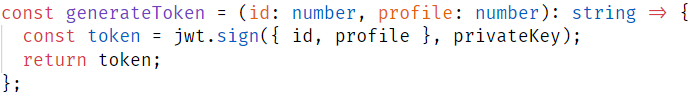
\includegraphics[width=0.80\textwidth]{dados/figuras/Proposta/Códigos/code_generate_token.png}
    \caption{Geração de Tokens usando JWT}
    \label{fig:codigoGeradorDeToken}
\end{figure}

A Figura \ref{fig:codigoValidadorDeToken} mostra a validação dos tokens recebidos. A função de validação funciona como um \textit{middleware} que recebe os dados da requisição recebidos por um consumidor, e tenta encontrar o Token no Header da requisição. Caso encontre o token, e o mesmo seja válido, o sistema continua a operação. Caso o token exista, porém seja inválido, o sistema bloqueia a requisição e envia uma mensagem de token inválido. E caso não haja token, a requisição é bloqueada com a mensagem de token inexistente.

\begin{figure}[H]
    \centering
    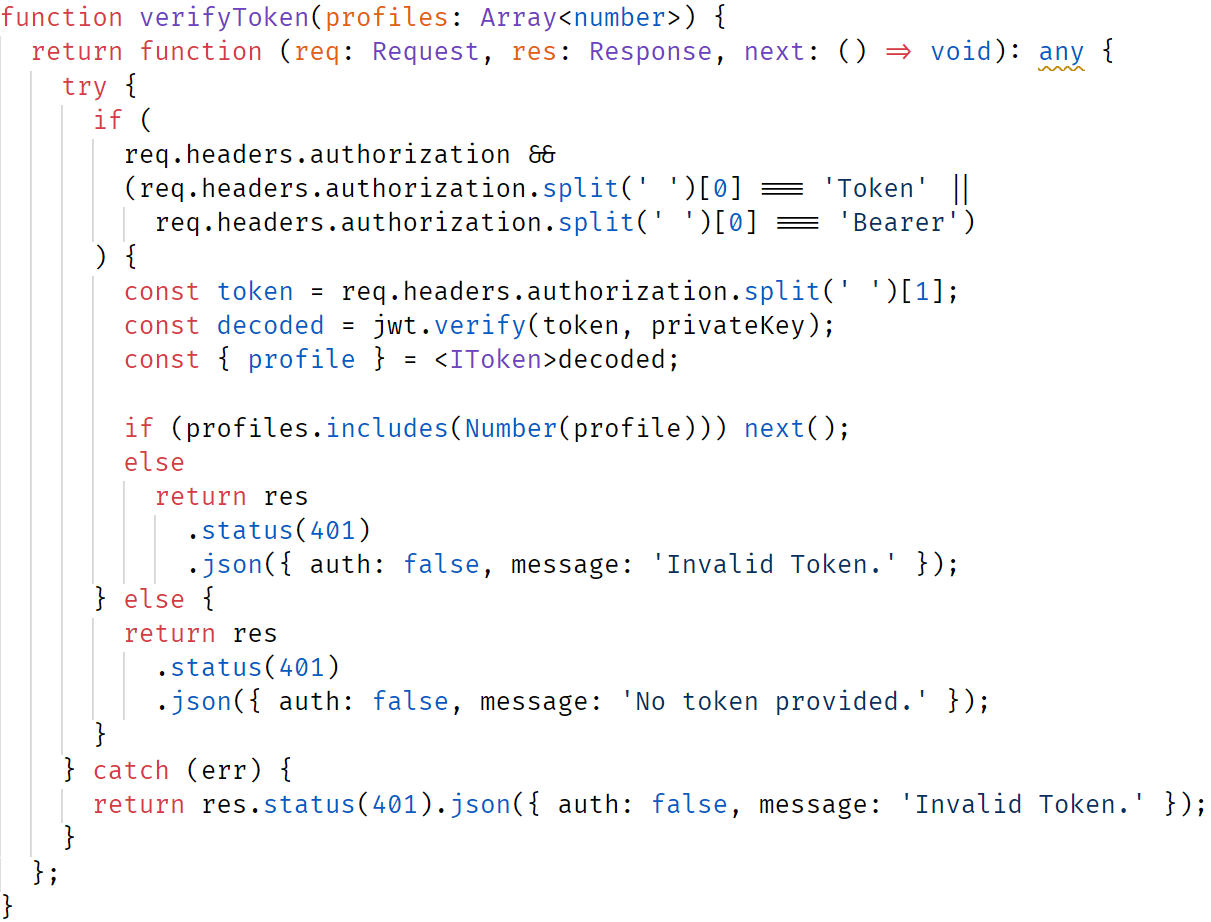
\includegraphics[width=\textwidth]{dados/figuras/Proposta/Códigos/code_validate_token.png}
    \caption{Geração de Tokens usando JWT}
    \label{fig:codigoValidadorDeToken}
\end{figure}


\subsection{\textit{Front-end}}

\cite{roveda2018frontend} descreve \textit{\textit{Front-end}} como toda parte da programação relativa à interface de uma aplicação e com o qual o usuário é capaz de interagir com o sistema. O \textit{\textit{Front-end}} KeeMe, como foi construído utilizando como base a biblioteca React que como descrito por sua documentação em \cite{react} se trata de uma biblioteca JavaScript para construção de interfaces. Em conjunto ao React, optou-se por utilizar também a biblioteca ChakraUI, que é "uma biblioteca de componentes simples, modular e acessível que fornece os blocos de construção de que você precisa para construir seus aplicativos React" \cite{chakraui}. A etapa de criação do \textit{\textit{Front-end}} buscou criar uma interface que fosse simples e de fácil utilização de forma que os usuários pudessem utilizá-la sem a necessidade de intervenção ou de tutoriais, além isso utilizou-se uma palheta de cores com a predominância do verde, que na psicologia das cores descrita por \cite{clemente2020cores} está relacionada à sensação de relaxamento e harmonia, dessa forma a interface busca passar ao usuário a sensação de relaxamento durante a utilização do sistema.

\begin{figure}[H]
    \centering
    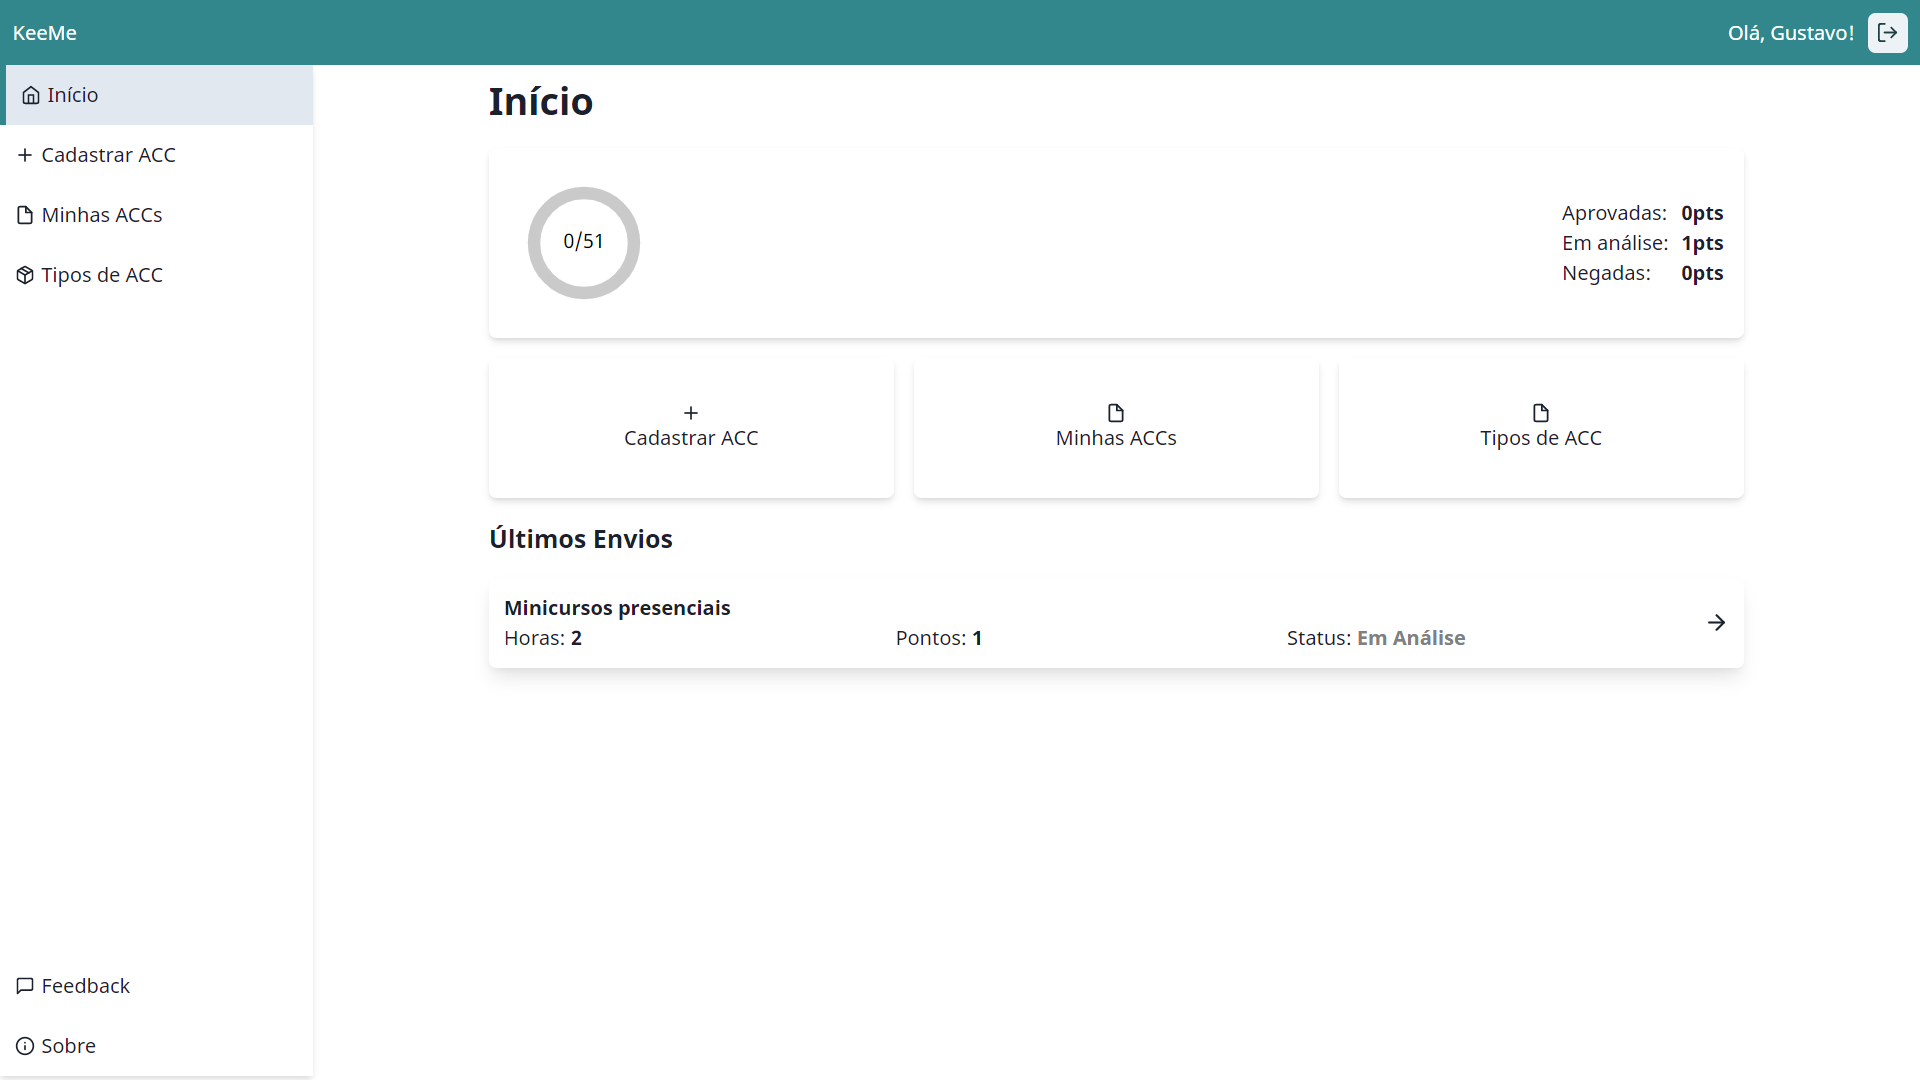
\includegraphics[width=\textwidth]{dados/figuras/Proposta/Screens/student_dashboard.png}
    \caption{Tela de Início do Discente}
    \label{fig:screenDashboardDiscente}
\end{figure}

A Figura \ref{fig:screenDashboardDiscente} mostra a tela de início de um usuário do tipo Discente, essa tela possui um resumo de todos os dados do discente. Trazendo um gráfico que mostra o avanço do discente em relação à conclusão da pontuação de ACC assim como a quantidade de pontos Aprovados, Em análise e Negados. Também são mostradas as principais funcionalidades do sistema, sendo estas Cadastrar ACC, Minhas ACCs e Tipos de ACC, além de uma seção com os últimos envios realizados pelo discente.

\begin{figure}[H]
    \centering
    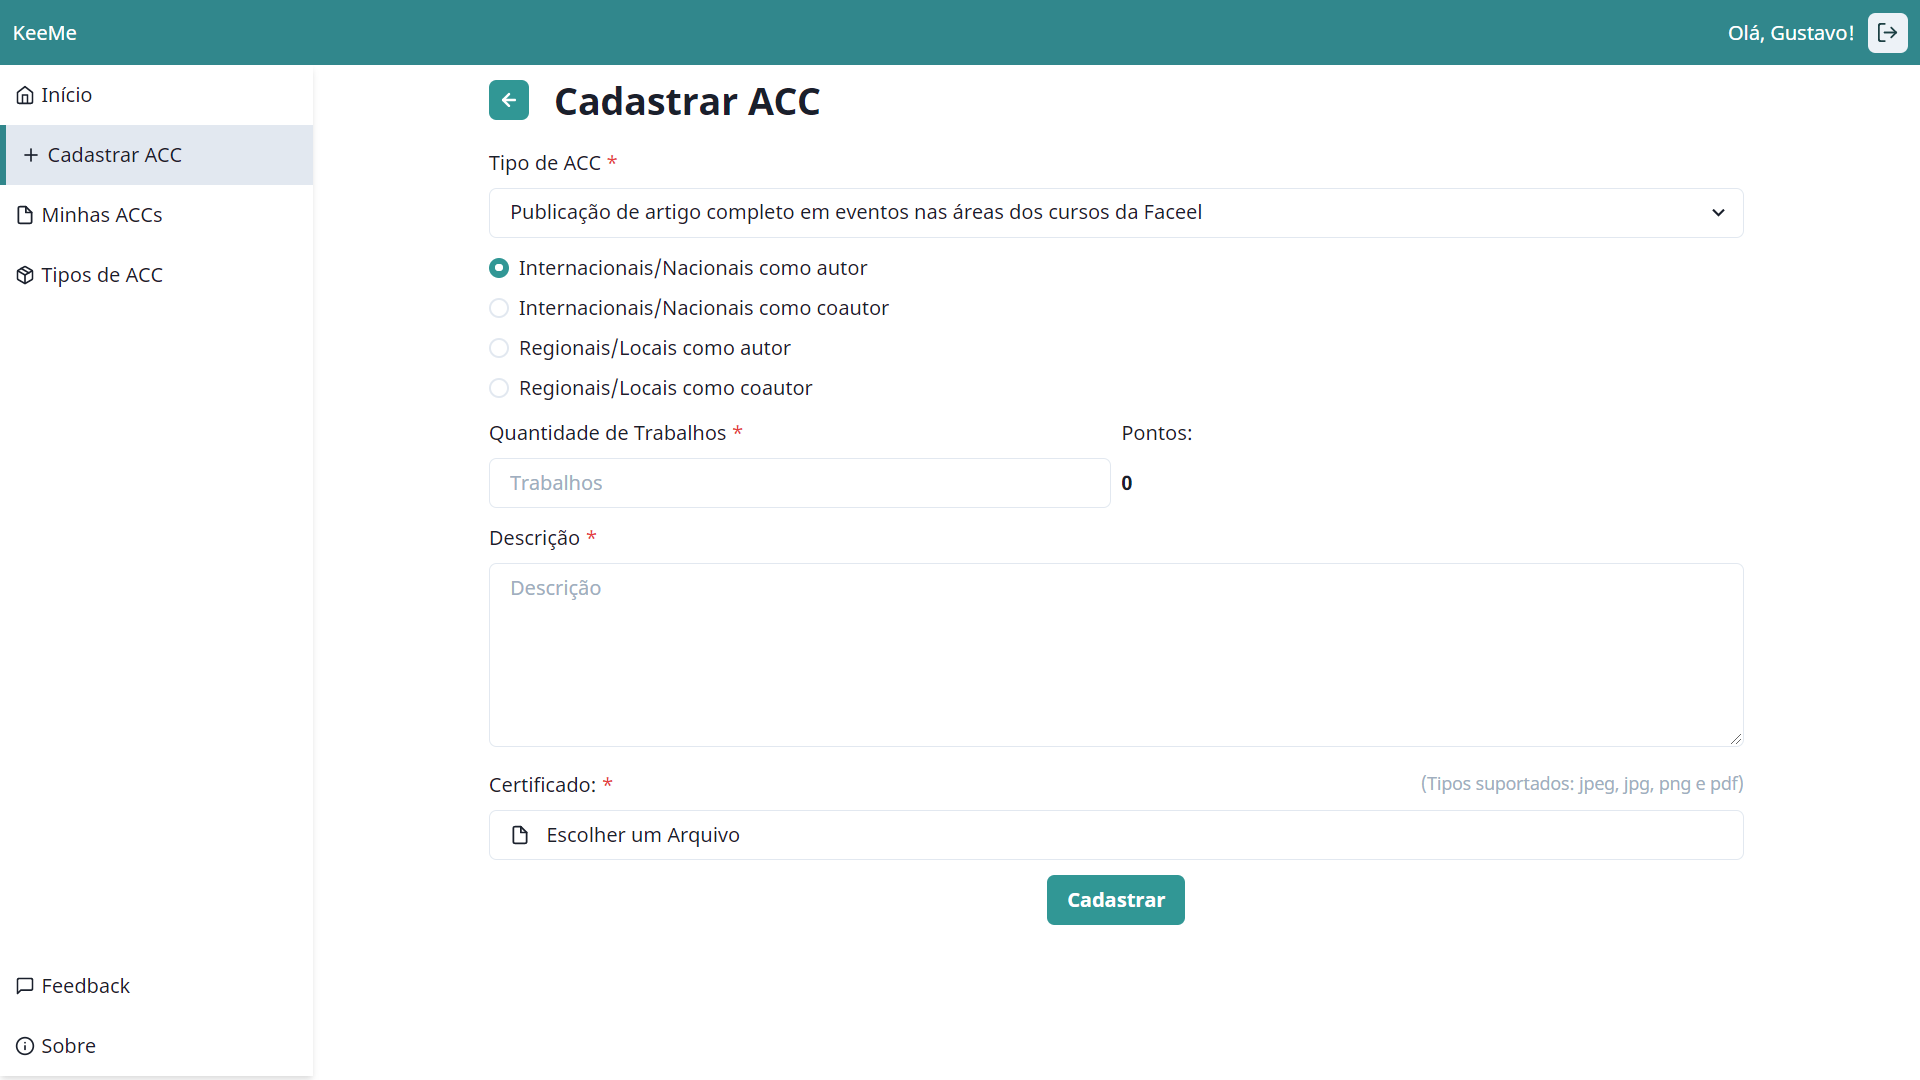
\includegraphics[width=\textwidth]{dados/figuras/Proposta/Screens/student_acc_request.png}
    \caption{Tela de Cadastro de ACC}
    \label{fig:screenCadastrarACC}
\end{figure}

Na Figura \ref{fig:screenCadastrarACC} é mostrada a tela de cadastro de uma ACC realizada pelo discente. O discente deve escolher um Tipo de ACC, e caso haja variações (Relacionado aos cursos da Faceel ou Não Relacionado aos cursos da Faceel, Congresso Regional ou Nacional, entre outros), deve escolher entre as mesmas. Além disso, o discente deve preencher a quantidade de unidades (como horas, semestres, dentre outros) realizadas, escrever uma descrição sobre a ACC, ou seja, o que ele realizou na mesma e por último anexar um certificado referente à ACC.

\begin{figure}[H]
    \centering
    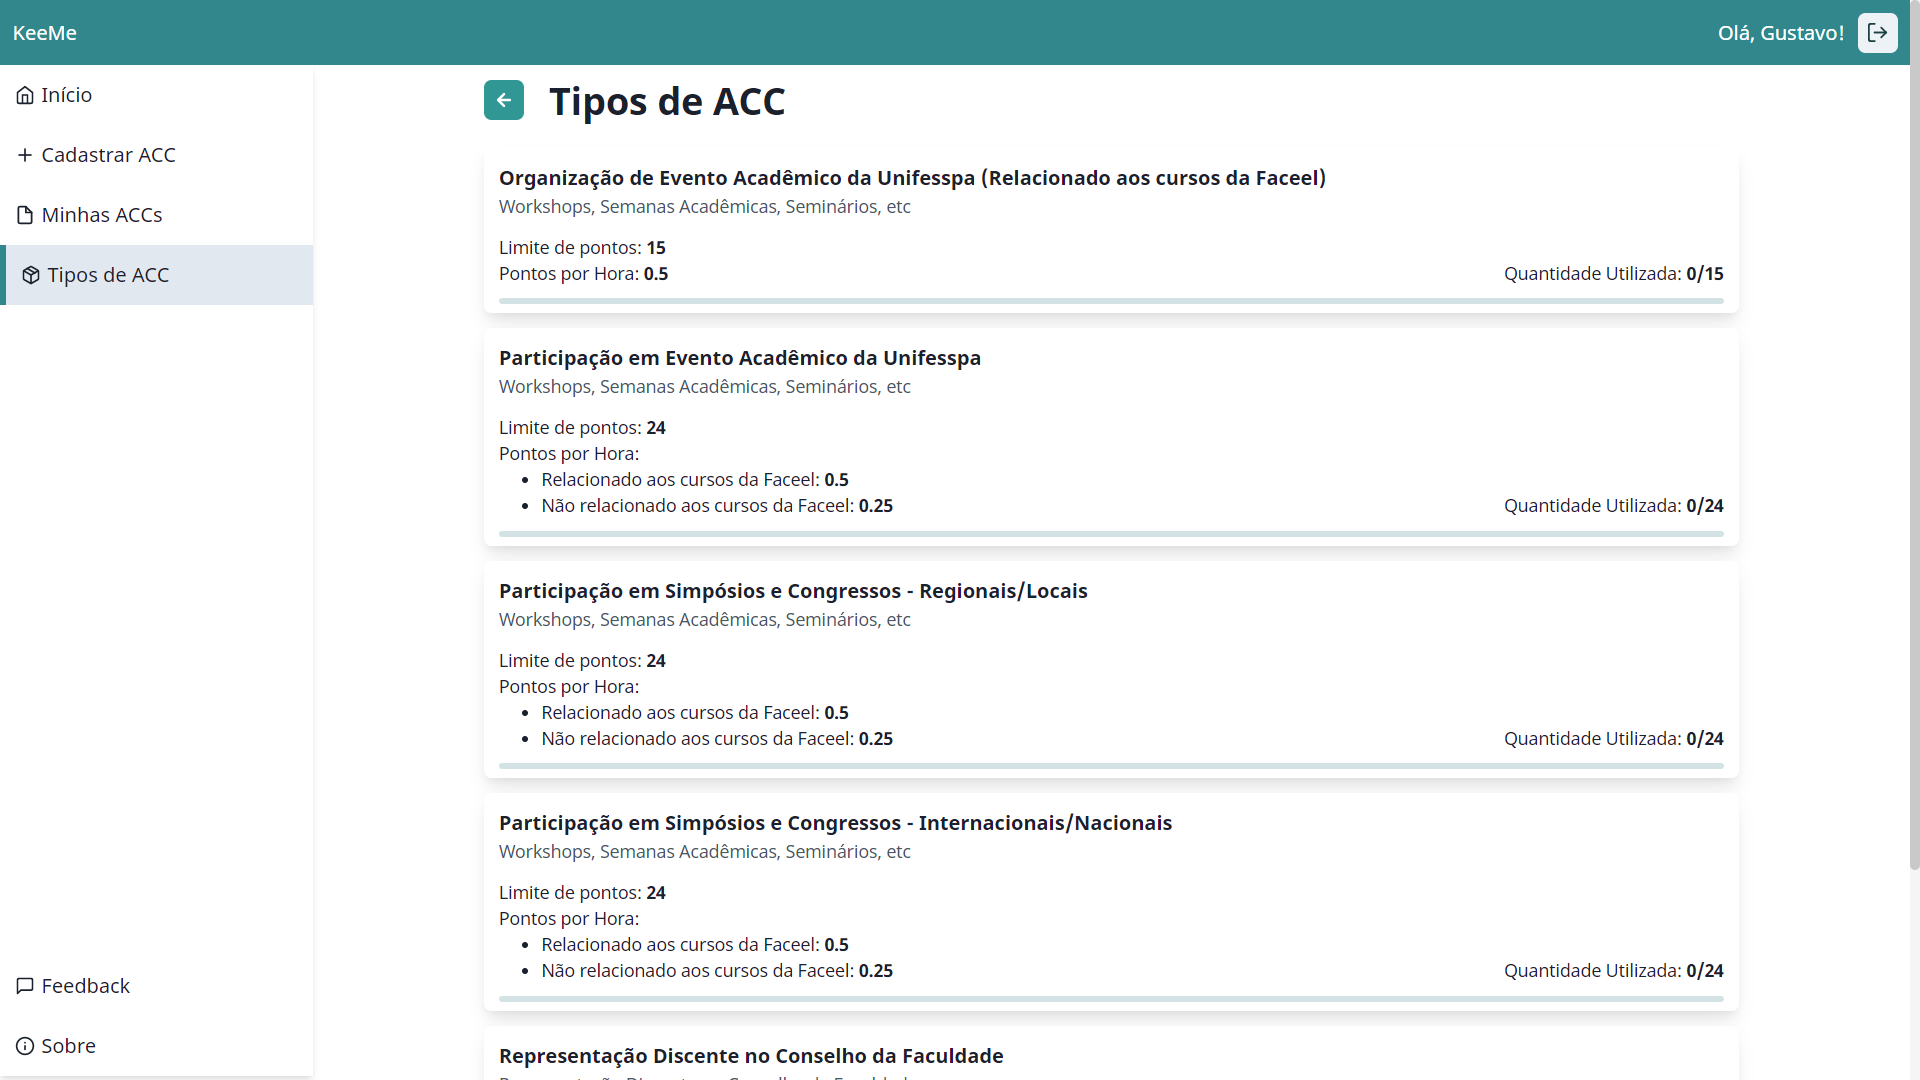
\includegraphics[width=\textwidth]{dados/figuras/Proposta/Screens/student_acc_types.png}
    \caption{Tela de Tipos de ACC}
    \label{fig:screenTiposDeACC}
\end{figure}

O discente poderá acessar os dados dos Tipos de ACC presentes no regulamento, assim como suas descrições, pontos por unidade e limites. Além disso, o discente poderá acompanhar visualmente quantos pontos o mesmo já conseguiu em determinado tipo de ACC, conforme mostrado na Figura \ref{fig:screenTiposDeACC}.

\begin{figure}[H]
    \centering
    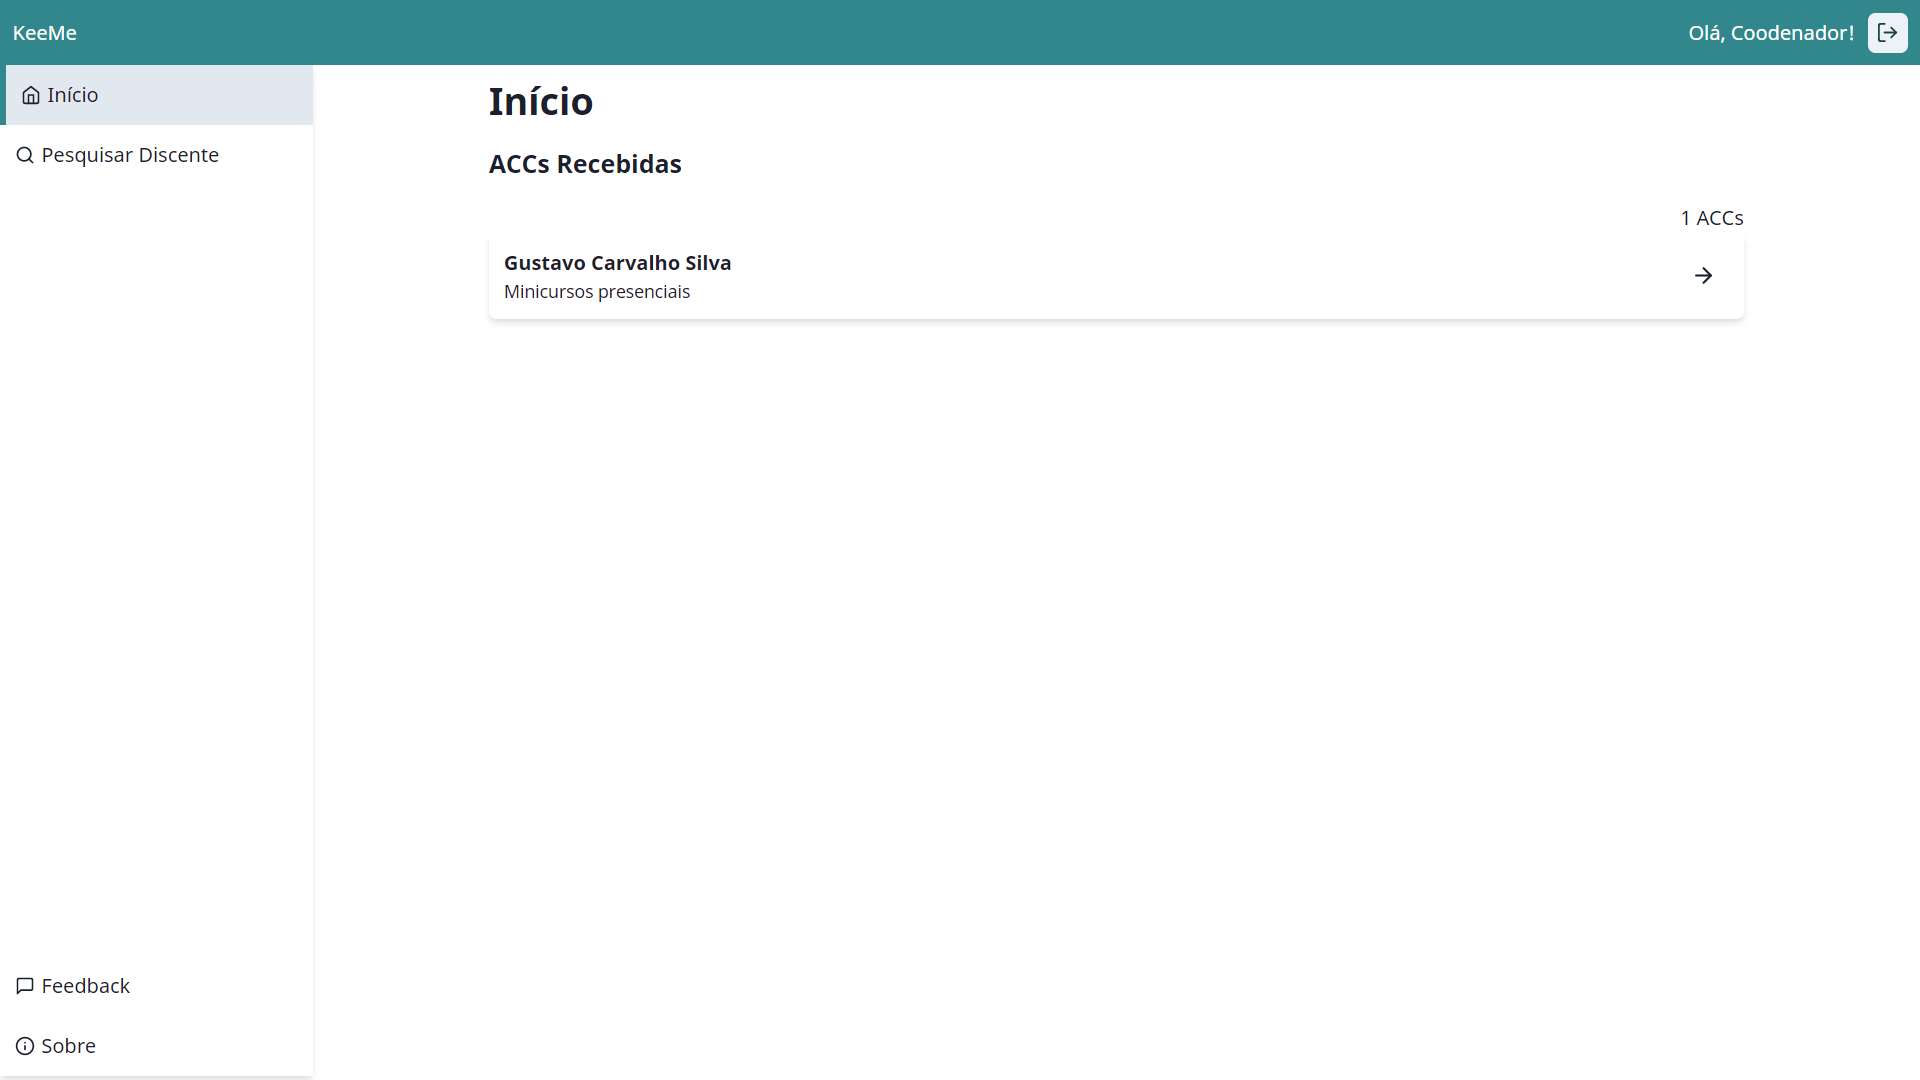
\includegraphics[width=0.9\textwidth]{dados/figuras/Proposta/Screens/coordinator_received_accs.png}
    \caption{Tela de Início do Coordenador}
    \label{fig:screenACCsRecebidas}
\end{figure}

A Figura \ref{fig:screenACCsRecebidas} mostra a tela de início de um usuário do tipo coordenador, conforme mostrado na imagem, o coordenador poderá ver as ACCs enviadas pelos discentes do curso ao qual ele está vinculado, além de uma contagem do número de ACCs que ainda precisam ser avaliadas.

\begin{figure}[H]
    \centering
    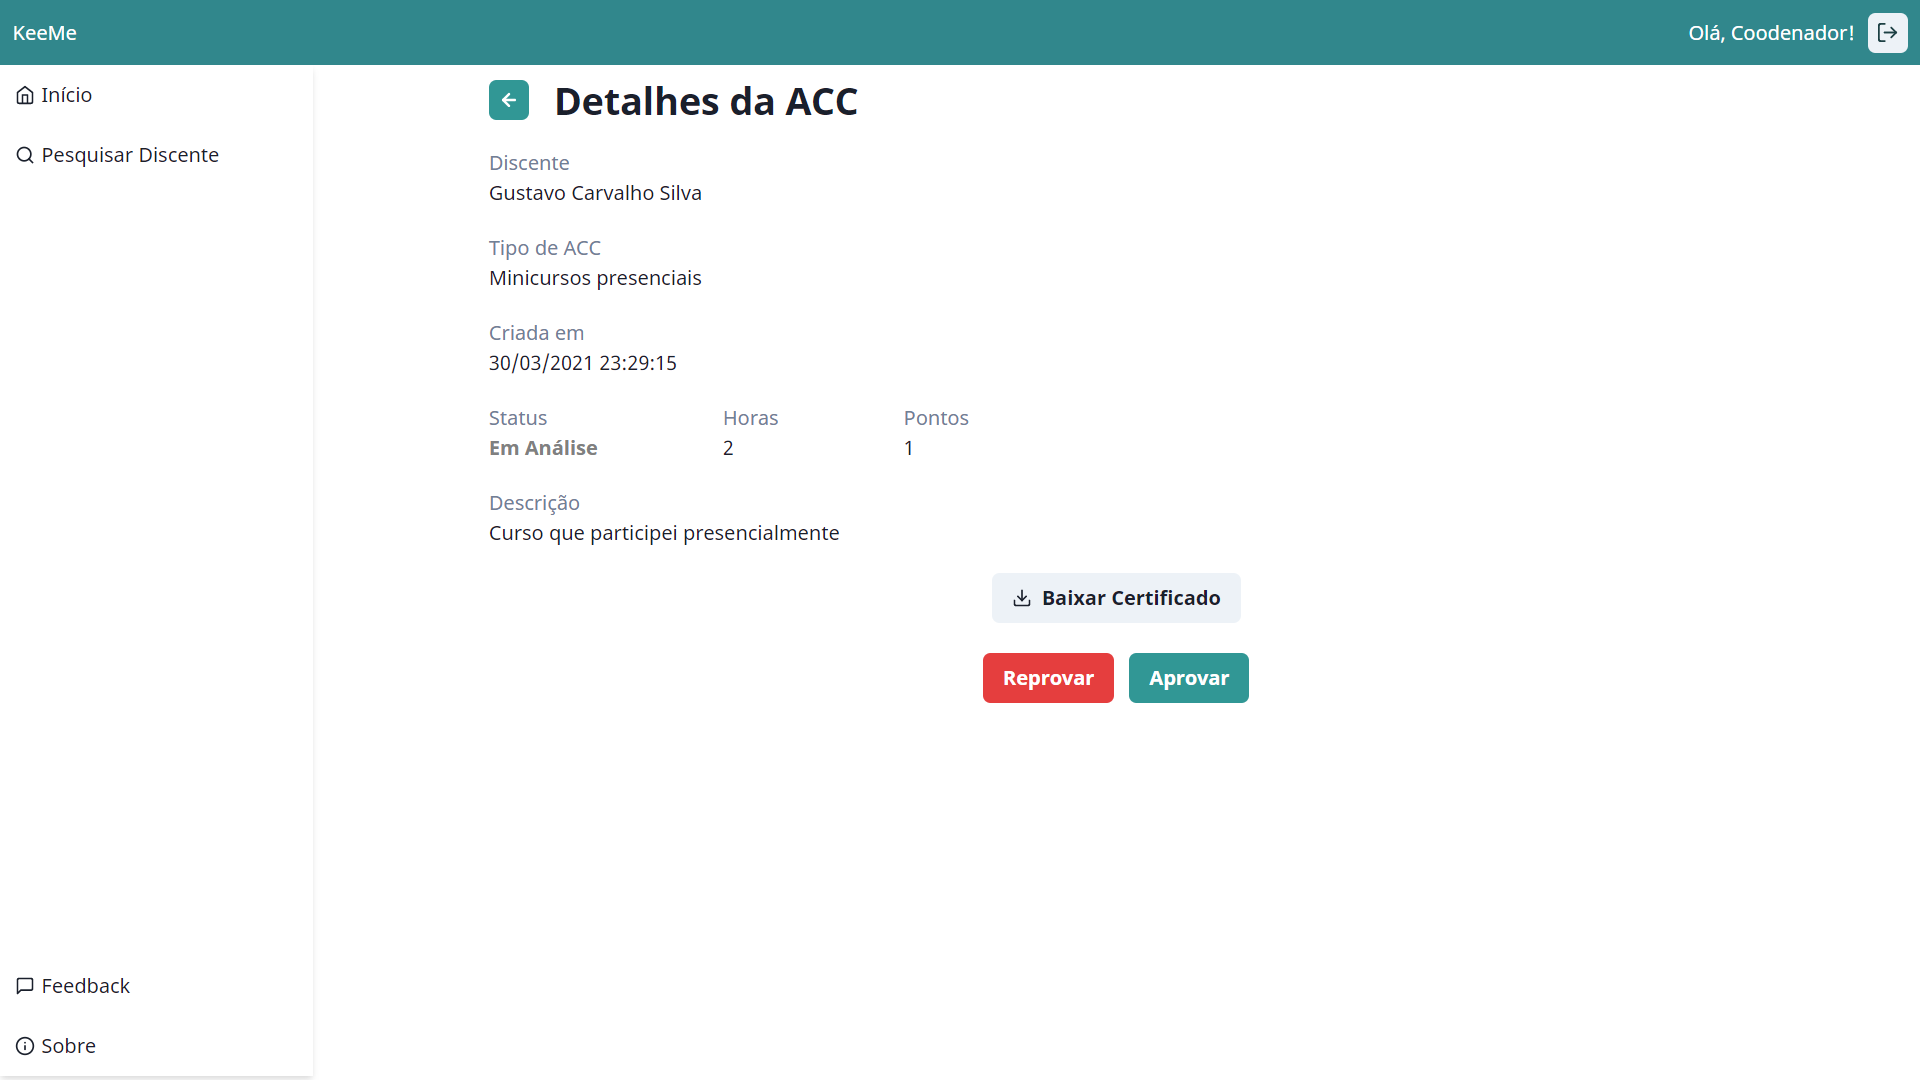
\includegraphics[width=0.9\textwidth]{dados/figuras/Proposta/Screens/evaluate_acc.png}
    \caption{Tela de Avaliação das ACCs}
    \label{fig:screenAvaliarACC}
\end{figure}

Na Figura \ref{fig:screenAvaliarACC} é possível ver a tela de avaliação de uma ACC. Como pode ser visto na imagem, além dos dados da ACC, o Coordenador poderá também baixar o certificado anexado. Após chegar a uma decisão, o Coordenador poderá aprovar a ACC ou reprová-la. No caso de uma reprovação, o coordenador deverá escrever o motivo da sua decisão.

\begin{figure}[H]
    \centering
    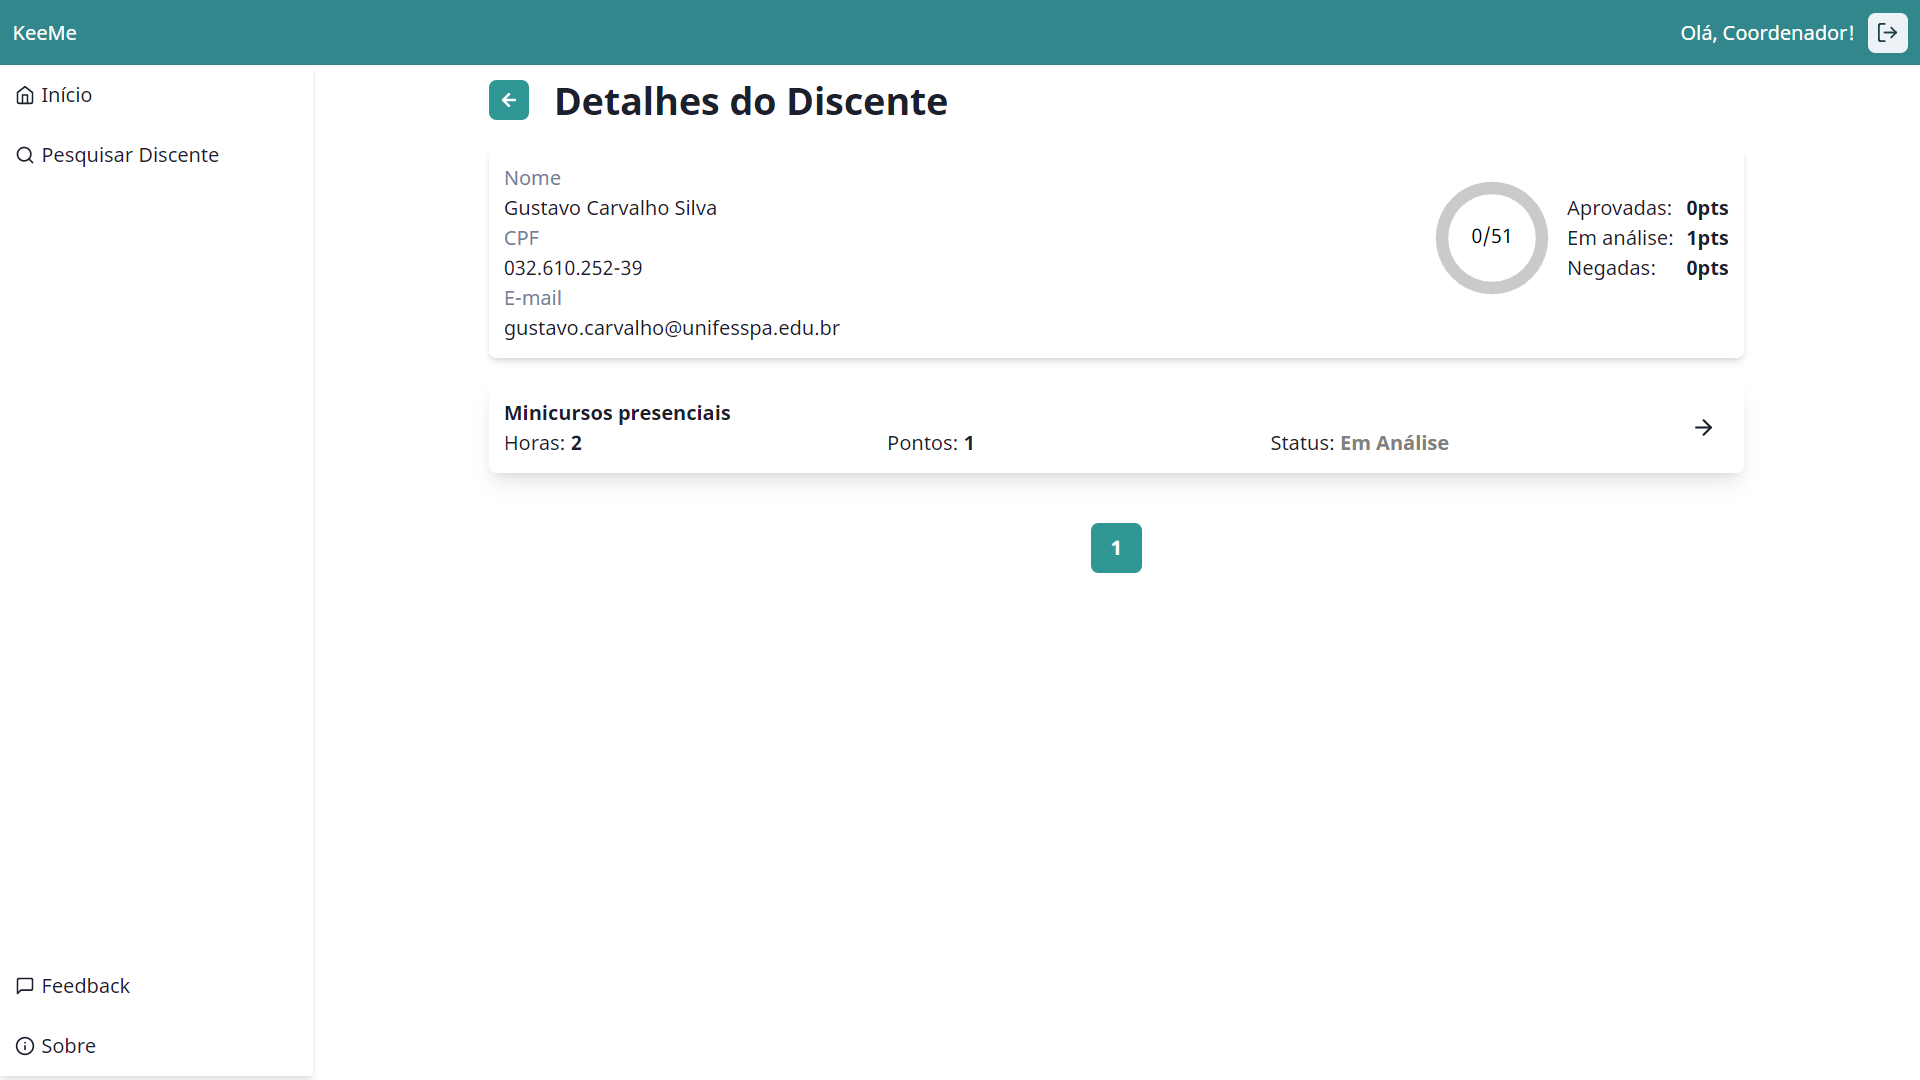
\includegraphics[width=\textwidth]{dados/figuras/Proposta/Screens/coordinator_student_details.png}
    \caption{Tela de Detalhes do Discente}
    \label{fig:screenDetalhesDoDiscente}
\end{figure}

O coordenador poderá acompanhar o avanço de um discente através da tela mostrada na Figura \ref{fig:screenDetalhesDoDiscente}. Essa tela exibe todas as informações pertinentes de um discente, além das informações de pontuação do mesmo. Sedo assim, é mostrado um gráfico que ilustra o avanço do discente na pontuação, e a quantidade de pontos que o mesmo possui para diferentes estados tais como, "Aprovados", "Reprovados" e "Em análise".

\begin{figure}[H]
    \centering
    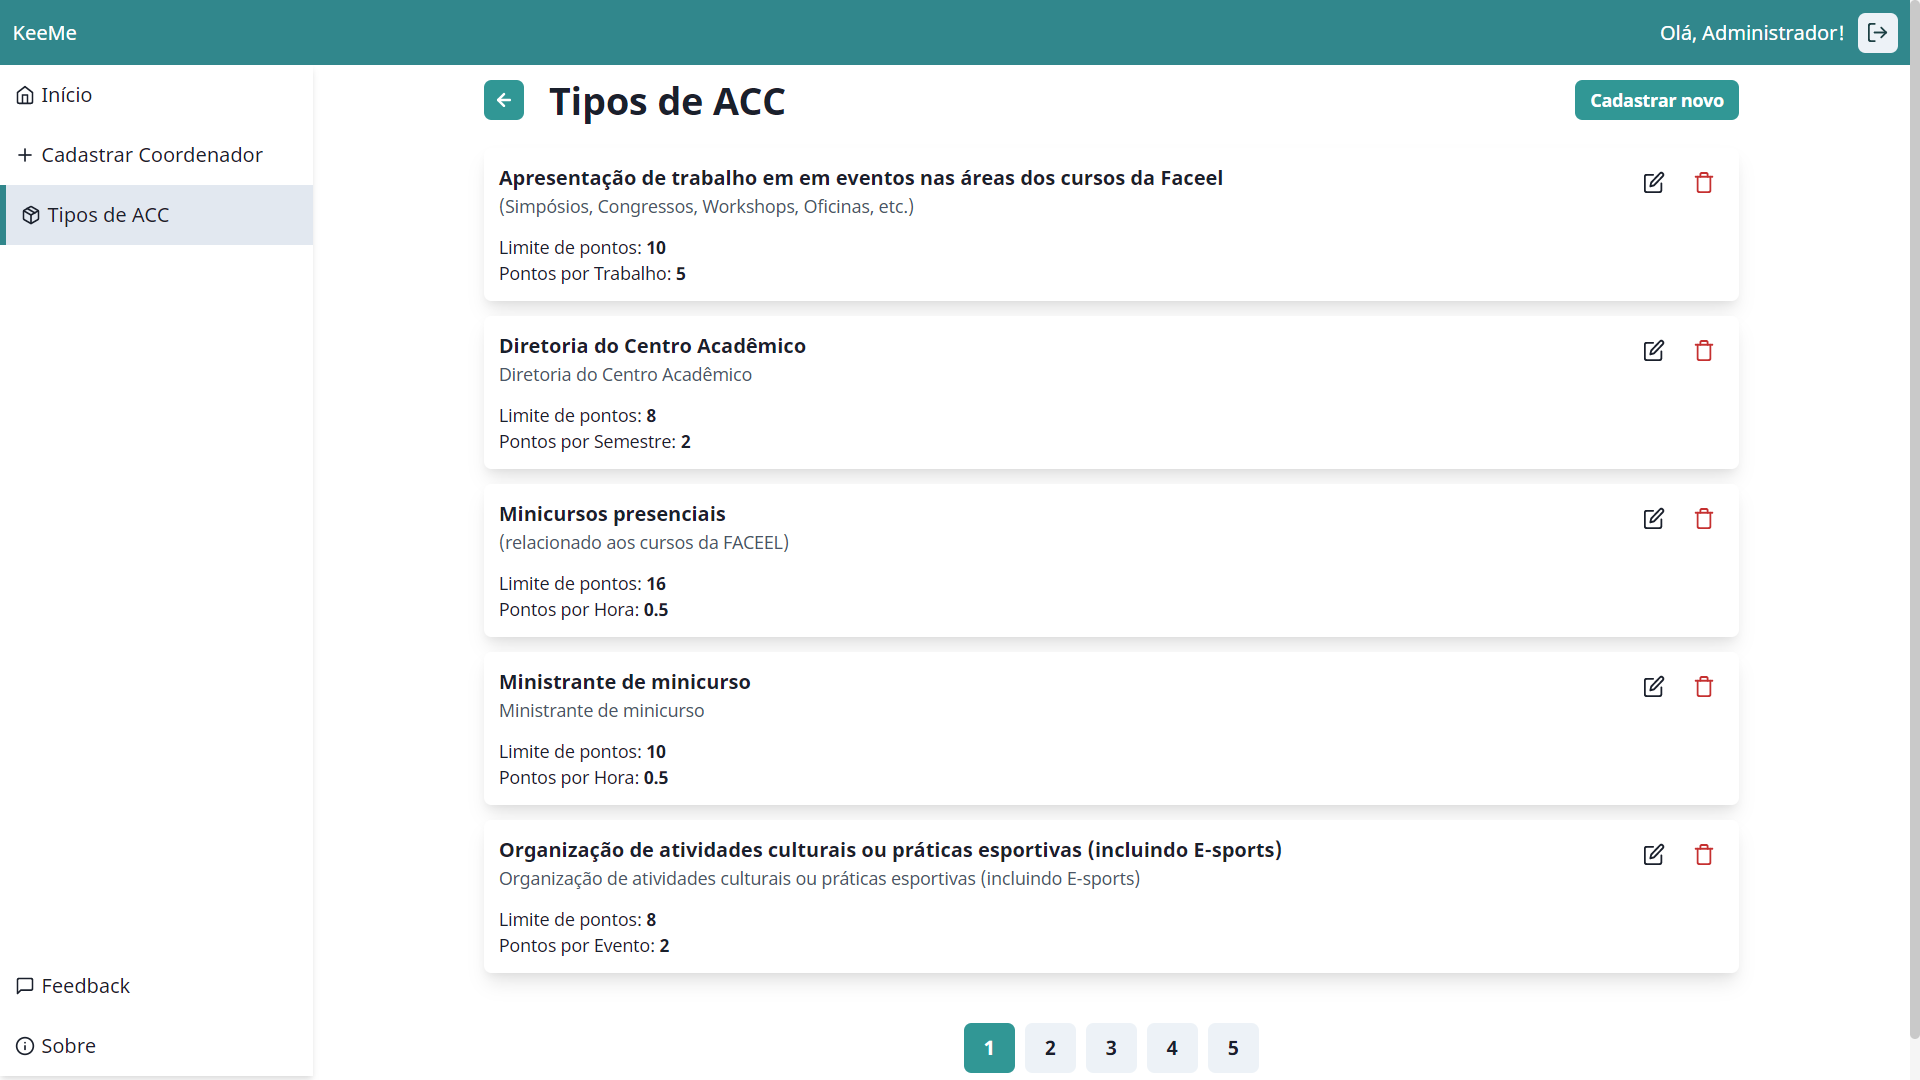
\includegraphics[width=\textwidth]{dados/figuras/Proposta/Screens/admin_acc_types.png}
    \caption{Tela de Listagem dos Tipos de ACC}
    \label{fig:screenListagemTiposDeACC}
\end{figure}

A Figura \ref{fig:screenListagemTiposDeACC} mostra a tela de listagem dos Tipos de ACC, esta tela se encontra dentro do módulo do Administrador e está baseada no caso de uso expandido da Tabela \ref{casoExpandido:gerenciarTiposDeACC}. Através dessa tela o Administrador tem acesso aos Tipos de ACC presentes dentro do sistema, além de poder realizar as operações de Cadastro, Consulta, Edição e Exclusão.

\begin{figure}[H]
    \centering
    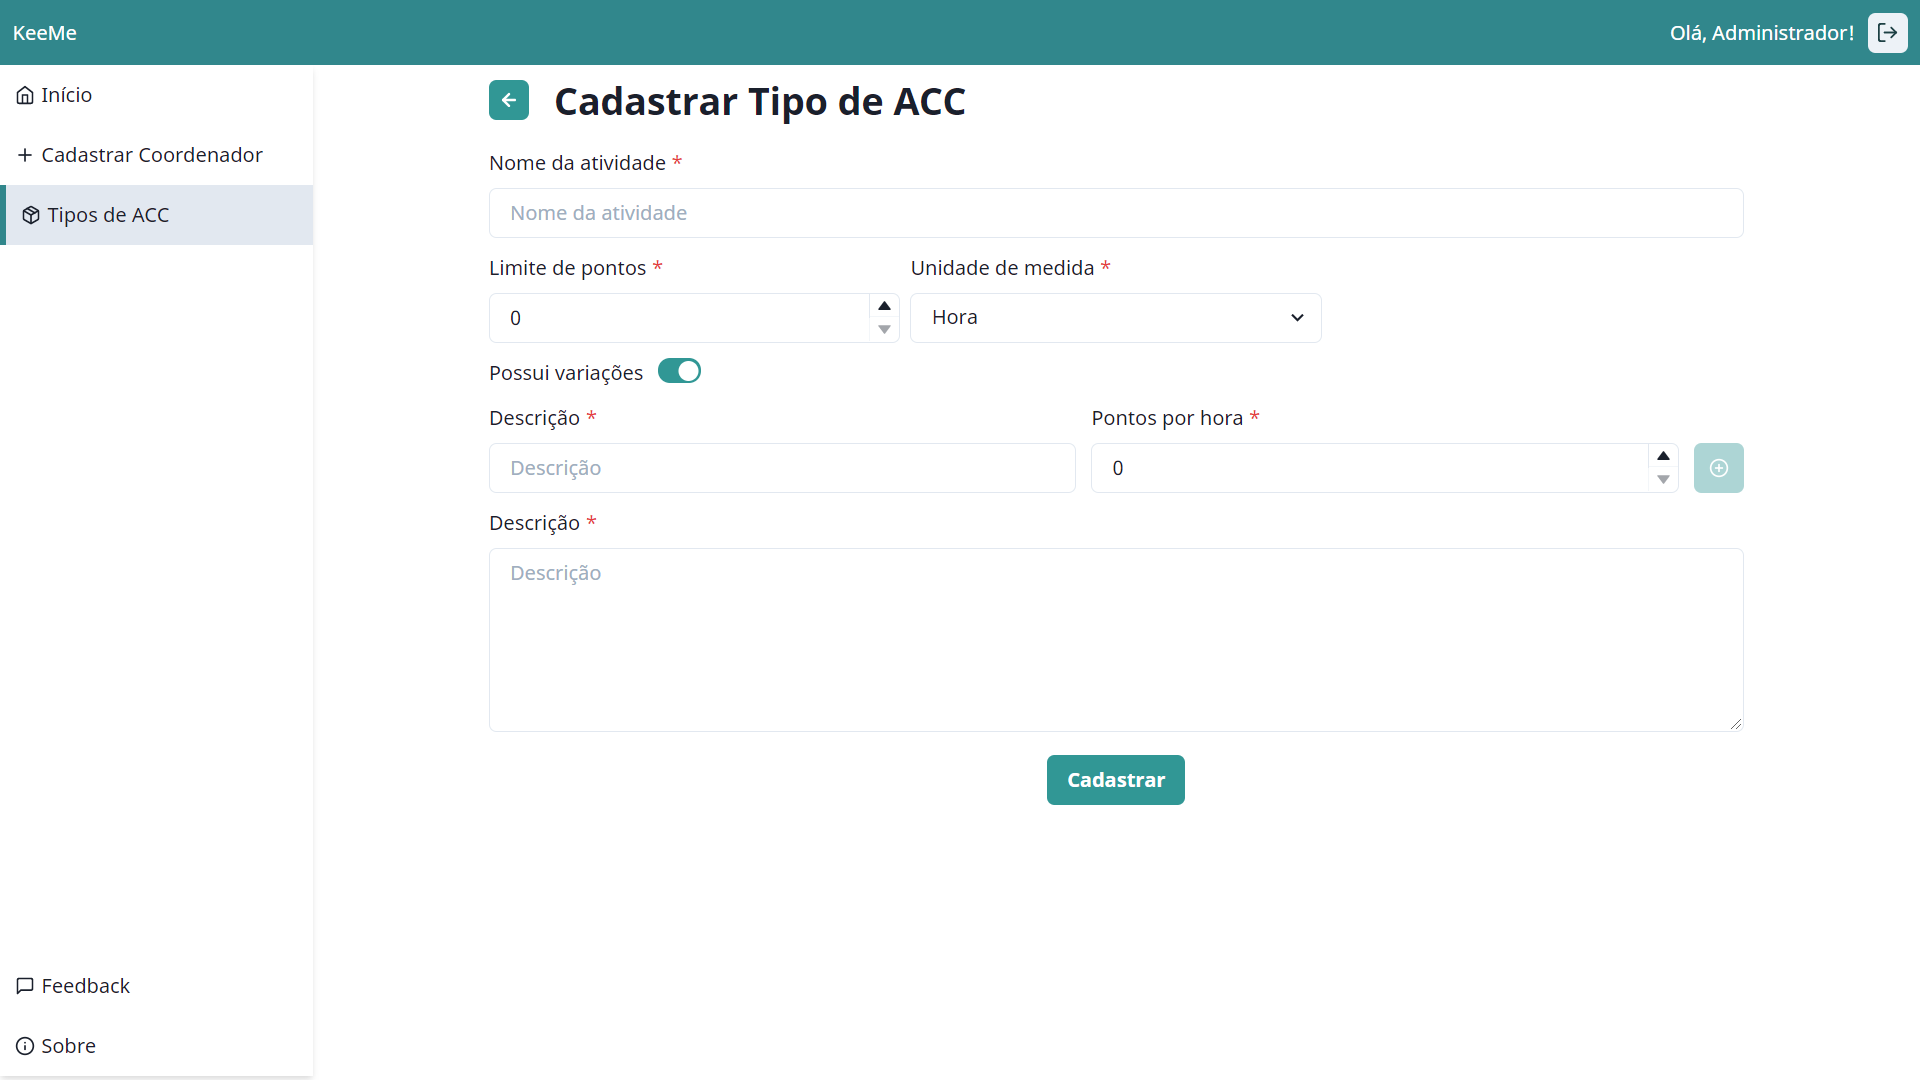
\includegraphics[width=\textwidth]{dados/figuras/Proposta/Screens/admin_create_acc_type.png}
    \caption{Tela de Cadastro de Tipo de ACC}
    \label{fig:screenCadastroTipoDeACC}
\end{figure}

Na Figura \ref{fig:screenCadastroTipoDeACC} é possível ver a tela de Cadastro de um novo Tipo de ACC, ação realizada por um usuário do tipo Administrador. O Administrador deve preencher os campos: Nome da atividade; Limite de pontos, que descreve o máximo de pontos que um usuário pode obter no Tipo de ACC; Unidade de Medida, que é a forma em que o Tipo de ACC será pontuado, se por Horas, Semestres, Certificados, entre outros; Variações, que são as variantes que este Tipo de ACC pode possuir, como Congresso Regional ou Nacional, dentro dos cursos da FACEEL ou não, entre outros; e a descrição do Tipo de ACC; Como pode ser observado na Figura \ref{fig:screenCadastroTipoDeACC} há uma opção chamada "Possui variações", caso essa opção esteja desmarcada o sistema não exibirá os campos para se adicionar as variantes, ficando apenas o campo de número de Pontos por unidade de medida, dessa forma, o Tipo de ACC será salvo sem variações.



% RESULTADOS-------------------------------------------------------------------

\chapter{ANÁLISE E DISCUSSÃO DOS RESULTADOS}
\label{chap:resultados}

A conceitualização de qualidade é complexa dada sua subjetividade, o mesmo se aplica a qualidade de software. \cite{morais2010qualidade} escreve em seu trabalho que a qualidade está associada a uma série de ações que devem ser executas dentro de uma organização com o fim de criar um produto que satisfaça às expectativas dos clientes. \cite{morais2010qualidade} descreve ainda que no contexto de software a qualidade pode ser vista como um conjunto de características que devem ser criadas para satisfazer as necessidades do usuário.

Neste capítulo, são mostrados resultados da avaliação de qualidade da aplicação KeeMe. A Seção \ref{sec:lighthouse} irá abordar sobre os resultados da avaliação feita utilizando a ferramenta Lighthouse, que é representada em \cite{lighthouse} como uma ferramenta de testes automatizados de qualidade de páginas web, que mostra numa escala de 0 a 100 o quanto uma aplicação web segue determinados requisitos de qualidade.


\section{Avaliação de Qualidade Utilizando Lighthouse}
\label{sec:lighthouse}

Com já foi abordado, o Lighthouse, segundo \cite{lighthouse} se trata de uma ferramenta de código aberto que realiza testes automatizados de qualidade em páginas web. Seus critérios de avaliação são:

\begin{itemize}
    \item Desempenho: avalia o desempenho geral de uma página, como o tempo que leva para que ela seja carregada pela primeira vez, o tempo até que se possa interagir com os elementos da tela, entre outros fatores;
    \item Acessibilidade: se refere aos parâmetros de acessibilidade utilizados durante a criação do código HTML e da interface de uma página. Esses parâmetros são o tamanho da fonte, o contraste entre a cor das fontes e do plano de fundo, entre outros fatores;
    \item SEO (\textit{Search Engine Optimization}): avalia a capacidade que uma aplicação possui de ser indexada por um motor de busca, como o Google. Em outras palavras, se refere à capacidade que uma aplicação possui de poder ser encontrada por buscadores;
    \item Práticas Recomendadas: este critério está ligado ao índice de boas práticas que foram seguidas na construção da página. Essas boas práticas incluem não mostrar erros no console dos navegadores, tornar a página rápida, tornar a página segura, entre outros;
\end{itemize}

O Lighthouse avalia esses fatores, e então pontua de 0 a 100 a página web, mostrando também o que levou àquela nota. O \cite{lighthouse} classifica as notas como sendo: 0 a 49, como "Desempenho Pobre", ou seja, sem muita qualidade; 50 a 89, como "Necessita de Melhoria", significa que a aplicação possui qualidade, mas precisa ser melhorada; e de 90 a 100 como "Bom", ou seja, a aplicação possui qualidade no critério avaliado. Essa ferramenta foi utilizada por conta da necessidade de se ter uma avaliação precisa da qualidade da aplicação, além de se ter um norteador do que poderia ser feito para que possa ser melhorada.

A Figura \ref{fig:graficoResultadosDesktop} mostra a média de resultados da avaliação de todas as telas acessadas através de um computador, para isso, acessou-se cada uma das telas, fazendo uma avaliação da qualidade e registrando os resultados, esses resultados foram então somados e divididos pela quantidade total de telas proporcionando a média entre elas. Como é possível ver no gráfico, todos os resultados ficaram acima dos 90 pontos, indicando que a aplicação segue os melhores critérios de qualidade. O Desempenho foi pontuado com 96,63; já Acessibilidade 96,55; enquanto SEO 99,75; e Boas Práticas 100.

\begin{figure}[H]
    \centering
    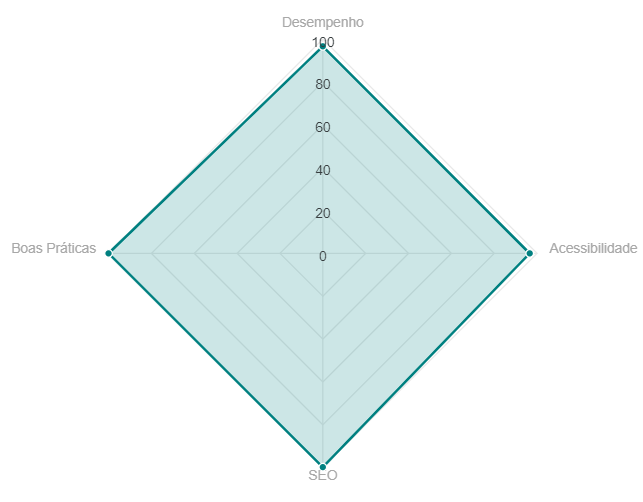
\includegraphics[width=12cm]{dados/figuras/Resultados/radar_desktop.png}
    \caption{Média de Resultados do Acesso por Computador}
    \label{fig:graficoResultadosDesktop}
\end{figure}

A Figura \ref{fig:graficoResultadosMobile} mostra a média de resultados da avaliação de todas as telas acessadas através de um dispositivo móvel, para se obter essa média foi realizado o teste de todas as telas do sistema através de um dispositivo móvel, após isso os resultados foram registrados, somados e divididos pela quantidade total de telas proporcionando a média de qualidade entre elas. Através do gráfico é possível ver que enquanto todos os outros resultados ficaram acima dos 90, o Desempenho ficou entre 70 e 80, o que indica que a aplicação possui um bom desempenho, mas que este ainda precisa ser melhorado no que diz respeito ao acesso por um dispositivo móvel. Sendo assim, as médias das notas foram: Desempenho, 75,27; Acessibilidade, 96,55; SEO, 99,75; e Boas Práticas, 99,75;

\begin{figure}[H]
    \centering
    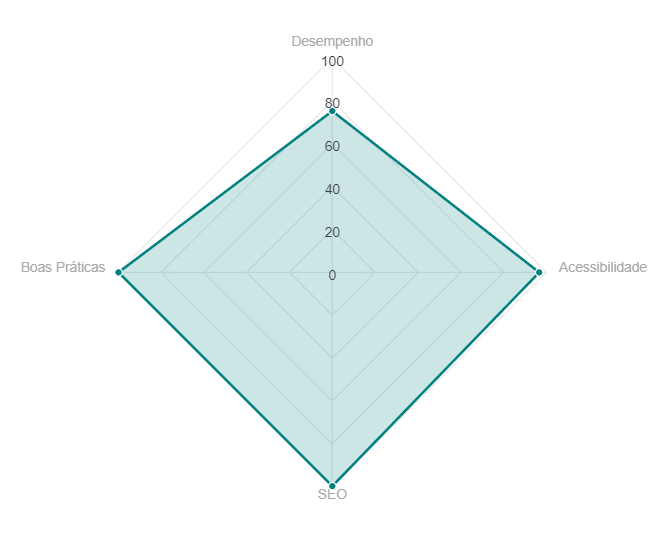
\includegraphics[width=12cm]{dados/figuras/Resultados/radar_mobile.png}
    \caption{Média de Resultados do Acesso por Dispositivo Móvel}
    \label{fig:graficoResultadosMobile}
\end{figure}

Como podemos ver nos resultados, a aplicação possui bons índices de qualidade tanto no acesso por um computador quanto no acesso por um dispositivo móvel. Como mostrado no gráfico da Figura \ref{fig:graficoResultadosMobile} o desempenho nos dispositivos móveis ainda precisa ser melhorado, tal resultado está ligado à utilização do React, ferramenta retratada em \cite{react} como sendo um \textit{framework} de criação de interfaces HTML usando Javascript. O React faz o carregamento de todo o \textit{script} gerado durante o primeiro acesso, para se melhorar a performance é necessário que seja feita uma estratégia de carregamento dinâmico desse \textit{script}.

 % Resultados

% % ORIENTAÇÕES GERAIS------------------------------------------------------------


% SOBRE AS ILUSTRAÇÕES----------------------------------------------------------
\chapter{SOBRE AS ILUSTRAÇÕES}
\label{chap:apSobreIlust}

A seguir exemplifica-se como inserir ilustrações no corpo do trabalho. As ilustrações serão indexadas automaticamente em suas respectivas listas. A numeração sequencial de figuras, tabelas e equações também ocorre de modo automático.

Referências cruzadas são obtidas através dos comandos \verb|\label{}| e \verb|\ref{}|. Sendo assim, não é necessário por exemplo, saber que o número de certo capítulo é \ref{chap:fundamentacaoTeorica} para colocar o seu número no texto. Outra forma que pode ser utilizada é esta: \autoref{chap:fundamentacaoTeorica}, facilitando a inserção, remoção e manejo de elementos numerados no texto sem a necessidade de renumerar todos esses elementos.

% FIGURAS-----------------------------------------------------------------------
\chapter{FIGURAS}
\label{chap:figuras}

Exemplo de como inserir uma figura. A \autoref{fig:figura-exemplo1} aparece automaticamente na lista de figuras. Para saber mais sobre o uso de imagens no \LaTeX{} consulte literatura especializada \cite{Goossens2007}.

Os arquivos das figuras devem ser armazenados no diretório de "/dados".

\begin{figure}[!htb]
    \centering
    \caption{Exemplo de Figura}
    \includegraphics[width=0.5\textwidth]{./dados/figuras/figura1}
    \fonte{\citeonline{IRL2014}}
    \label{fig:figura-exemplo1}
\end{figure}

% QUADROS E TABELAS---------------------------------------------------------------
\chapter{QUADROS E TABELAS}
\label{chap:tabelas}

Exemplo de como inserir o \autoref{qua:quadro-exemplo1} e a \autoref{tab:tabela-exemplo1}. Ambos aparecem automaticamente nas suas respectivas listas. Para saber mais informações sobre a construção de tabelas no \LaTeX{} consulte literatura especializada \cite{Mittelbach2004}.

Ambos os elementos (Quadros e Tabelas) devem ser criados em arquivos separados para facilitar manutenção e armazenados no diretório de "/dados".

\begin{quadro}[!htb]
    \centering
    \caption{Exemplo de Quadro.\label{qua:quadro-exemplo1}}
    \begin{tabular}{|p{7cm}|p{7cm}|}
        \hline
        \textbf{BD Relacionais} & \textbf{BD Orientados a Objetos} \\
        \hline
        Os dados são passivos, ou seja, certas operações limitadas podem ser automaticamente acionadas quando os dados são usados. Os dados são ativos, ou seja, as solicitações fazem com que os objetos executem seus métodos. & Os processos que usam dados mudam constantemente. \\
        \hline
    \end{tabular}
    \fonte{\citeonline{Barbosa2004}}
\end{quadro}


A diferença entre quadro e tabela está no fato que um quadro é formado por linhas horizontais e verticais. Deve ser utilizado quando o conteúdo é majoritariamente não-numérico. O número do quadro e o título vem acima do quadro, e a fonte, deve vir abaixo. E Uma tabela é formada apenas por linhas verticais. Deve ser utilizada quando o conteúdo é majoritariamente numérico. O número da tabela e o título vem acima da tabela, e a fonte, deve vir abaixo, tal como no quadro.

\begin{table}[!htb]
    \centering
    \caption[Resultado dos testes]{Resultado dos testes.
    \label{tab:tabela-exemplo1}}
    \begin{tabular}{rrrrr}
        \toprule
            & Valores 1 & Valores 2 & Valores 3 & Valores 4 \\
        \midrule
            Caso 1 & 0,86 & 0,77 & 0,81 & 163 \\
            Caso 2 & 0,19 & 0,74 & 0,25 & 180 \\
            Caso 3 & 1,00 & 1,00 & 1,00 & 170 \\
        \bottomrule
    \end{tabular}
    \fonte{\citeonline{Barbosa2004}}
\end{table}


% EQUAÇÕES-----------------------------------------------------------------------
\chapter{EQUAÇÕES}
\label{chap:equacoes}

Exemplo de como inserir a \autoref{eq:equacao-exemplo1} e a Eq. \ref{eq:equacao-exemplo2} no corpo do texto \footnote{Deve-se atentar ao fato de a formatação das equações ficar muito boa esteticamente.}. Observe que foram utilizadas duas formas distintas para referenciar as equações.

\begin{equation}
    X(s) = \int\limits_{t = -\infty}^{\infty} x(t) \, \text{e}^{-st} \, dt
    \label{eq:equacao-exemplo1}
\end{equation}

\begin{equation}
    F(u, v) = \sum_{m = 0}^{M - 1} \sum_{n = 0}^{N - 1} f(m, n) \exp \left[ -j 2 \pi \left( \frac{u m}{M} + \frac{v n}{N} \right) \right]
    \label{eq:equacao-exemplo2}
\end{equation}

% ALGORITMOS-----------------------------------------------------------------------
\chapter{ALGORITMOS}
\label{chap:algoritmos}

Exemplo de como inserir um algoritmo. Para inserção de algoritmos utiliza-se o pacote {\ttfamily algorithm2e} que já está devidamente configurado dentro do template.

Os algoritmos devem ser criados em arquivos separados para facilitar manutenção e armazenados no diretório de "/dados".\\
\\

\begin{algorithm}
    \caption{Exemplo de Algoritmo}
    \KwIn{o número $n$ de vértices a remover, grafo original $G(V, E)$}
    \KwOut{grafo reduzido $G'(V,E)$}
    $removidos \leftarrow 0$ \\
    \While {removidos $<$ n } {
        $v \leftarrow$ Random$(1, ..., k) \in V$ \\
            \For {$u \in adjacentes(v)$} {
                remove aresta (u, v)\\
                $removidos \leftarrow removidos + 1$\\
            }
            \If {há  componentes desconectados} {
                remove os componentes desconectados\\
            }
        }
\end{algorithm}


% SOBRE AS LISTAS--------------------------------------------------------------------
\chapter{SOBRE AS LISTAS}
\label{chap:apSobreLista}

Para construir listas de "\textit{bullets}"{} ou listas enumeradas, inclusive listas aninhadas, é utilizado o pacote \verb|paralist|.

Exemplo de duas listas não numeradas aninhadas, utilizando o comando \verb|\itemize|. Observe a indentação, bem como a mudança automática do tipo de "\textit{bullet}"{} nas listas aninhadas.

\begin{itemize}
    \item item não numerado 1
    \item item não numerado 2
    \begin{itemize}
        \item subitem não numerado 1
        \item subitem não numerado 2
        \item subitem não numerado 3
    \end{itemize}
    \item item não numerado 3
\end{itemize}

Exemplo de duas listas numeradas aninhadas, utilizando o comando \verb|\enumerate|. Observe a numeração progressiva e indentação das listas aninhadas.

\begin{enumerate}
    \item item numerado 1
    \item item numerado 2
    \begin{enumerate}
        \item subitem numerado 1
        \item subitem numerado 2
        \item subitem numerado 3
    \end{enumerate}
    \item item numerado 3
\end{enumerate}

% SOBRE AS CITAÇÕES E CHAMADAS DE REFERÊNCAS----------------------------------------------
\chapter{SOBRE AS CITAÇÕES E CHAMADAS DE REFERÊNCAS}
\label{chap:apSobreCita}

Citações são trechos de texto ou informações obtidas de materiais consultadss quando da elaboração do trabalho. São utilizadas no texto com o propósito de esclarecer, completar e embasar as ideias do autor. Todas as publicações consultadas e utilizadas (por meio de citações) devem ser listadas, obrigatoriamente, nas referências bibliográficas, para preservar os direitos autorais. São classificadas em citações indiretas e diretas.

% CITAÇÕES INDIRETAS-----------------------------------------------------------------------
\chapter{CITAÇÕES INDIRETAS}
\label{chap:citacoesLivres}

É a transcrição, com suas próprias palavras, das idéias de um autor, mantendo-se o sentido original. A citação indireta é a maneira que o pesquisador tem de ler, compreender e gerar conhecimento a partir do conhecimento de outros autores. Quanto à chamada da referência, ela pode ser feita de duas maneiras distintas, conforme o nome do(s) autor(es) façam parte do seu texto ou não. Exemplo de chamada fazendo parte do texto:\\
\\Enquanto \citeonline{Maturana2003} defendem uma epistemologia baseada na biologia. Para os autores, é necessário rever \ldots.\\

A chamada de referência foi feita com o comando \verb|\citeonline{chave}|, que produzirá a formatação correta.

A segunda forma de fazer uma chamada de referência deve ser utilizada quando se quer evitar uma interrupção na sequência do texto, o que poderia, eventualmente, prejudicar a leitura. Assim, a citação é feita e imediatamente após a obra referenciada deve ser colocada entre parênteses. Porém, neste caso específico, o nome do autor deve vir em caixa alta, seguido do ano da publicação. Exemplo de chamada não fazendo parte do texto:\\
\\Há defensores da epistemologia baseada na biologia que argumentam em favor da necessidade de \ldots \cite{Maturana2003}.\\

Nesse caso a chamada de referência deve ser feita com o comando \verb|\cite{chave}|, que produzirá a formatação correta.

% CITAÇÕES DIRETAS-----------------------------------------------------------------------
\chapter{CITAÇÕES DIRETAS}
\label{chap:citacoesLiterais}

É a transcrição ou cópia de um parágrafo, de uma frase, de parte dela ou de uma expressão, usando exatamente as mesmas palavras adotadas pelo autor do trabalho consultado.

Quanto à chamada da referência, ela pode ser feita de qualquer das duas maneiras já mencionadas nas citações indiretas, conforme o nome do(s) autor(es) façam parte do texto ou não. Há duas maneiras distintas de se fazer uma citação direta, conforme o trecho citado seja longo ou curto.

Quando o trecho citado é longo (4 ou mais linhas) deve-se usar um parágrafo específico para a citação, na forma de um texto recuado (4 cm da margem esquerda), com tamanho de letra menor e espaçamento entrelinhas simples. Exemplo de citação longa:
\\\begin{citacao}
    Desse modo, opera-se uma ruptura decisiva entre a reflexividade filosófica, isto é a possibilidade do sujeito de pensar e de refletir, e a objetividade científica. Encontramo-nos num ponto em que o conhecimento científico está sem consciência. Sem consciência moral, sem consciência reflexiva e também subjetiva. Cada vez mais o desenvolvimento extraordinário do conhecimento científico vai tornar menos praticável a própria possibilidade de reflexão do sujeito sobre a sua pesquisa \cite[p.~28]{Silva2000}.
\end{citacao}

Para fazer a citação longa deve-se utilizar os seguintes comandos:
\begin{verbatim}
\begin{citacao}
<texto da citacao>
\end{citacao}
\end{verbatim}

No exemplo acima, para a chamada da referência o comando \verb|\cite[p.~28]{Silva2000}| foi utilizado, visto que os nomes dos autores não são parte do trecho citado. É necessário também indicar o número da página da obra citada que contém o trecho citado.

Quando o trecho citado é curto (3 ou menos linhas) ele deve inserido diretamente no texto entre aspas. Exemplos de citação curta:\\
\\A epistemologia baseada na biologia parte do princípio de que "assumo que não posso fazer referência a entidades independentes de mim para construir meu explicar" \cite[p.~35]{Maturana2003}.\\
\\A epistemologia baseada na biologia de \citeonline[p.~35]{Maturana2003} parte do princípio de que "assumo que não posso fazer referência a entidades independentes de mim para construir meu explicar".

% DETALHES SOBRE AS CHAMADAS DE REFERÊNCIAS---------------------------------------------------------
\chapter{DETALHES SOBRE AS CHAMADAS DE REFERÊNCIAS}
\label{chap:referUtilizadas}

Outros exemplos de comandos para as chamadas de referências e o resultado produzido por estes:\\
\\\citeonline{Maturana2003} \ \ \  \verb|\citeonline{Maturana2003}|\\
\citeonline{Barbosa2004} \ \ \   \verb|\citeonline{Barbosa2004}|\\
\cite[p.~28]{Silva2000} \ \ \  \verb|\cite[p.~28]{Silva2000}|\\
\citeonline[p.~33]{Silva2000} \ \ \   \verb|\citeonline[p.~33]{v}|\\
\cite[p.~35]{Maturana2003} \ \ \   \verb|\cite[p.~35]{Maturana2003}|\\
\citeonline[p.~35]{Maturana2003} \ \ \   \verb|\citeonline[p.~35]{Maturana2003}|\\
\cite{Barbosa2004,Maturana2003} \ \ \   \verb|\cite{Barbosa2004,Maturana2003}|\\

% SOBRE AS REFERÊNCIAS BIBLIOGRÁFICAS-------------------------------------------------------
\chapter{SOBRE AS REFERÊNCIAS BIBLIOGRÁFICAS}
\label{chap:apSobreRefer}

A bibliografia é feita no padrão \textsc{Bib}\TeX{}. As referências são colocadas em um arquivo separado. Neste template as referências são armazenadas no arquivo "base-referencias.bib".

Existem diversas categorias documentos e materiais componentes da bibliografia. A classe abn\TeX{} define as seguintes categorias (entradas):

\begin{verbatim}
@book
@inbook
@article
@phdthesis
@mastersthesis
@monography
@techreport
@manual
@proceedings
@inproceedings
@journalpart
@booklet
@patent
@unpublished
@misc
\end{verbatim}

Cada categoria (entrada) é formatada pelo pacote \citeonline{abnTeX22014d} de uma forma específica. Algumas entradas foram introduzidas especificamente para atender à norma \citeonline{NBR6023:2002}, são elas: \verb|@monography|, \verb|@journalpart|,\verb|@patent|. As demais entradas são padrão \textsc{Bib}\TeX{}. Para maiores detalhes, refira-se a \citeonline{abnTeX22014d}, \citeonline{abnTeX22014b}, \citeonline{abnTeX22014c}.

% NOTAS DE RODAPÉ--------------------------------------------------------------------------
\chapter{NOTAS DE RODAPÉ}
\label{chap:notasRodape}

As notas de rodapé pode ser classificadas em duas categorias: notas explicativas\footnote{é o tipo mais comum de notas que destacam, explicam e/ou complementam o que foi dito no corpo do texto, como esta nota de rodapé, por exemplo.} e notas de referências. A notas de referências, como o próprio nome ja indica, são utilizadas para colocar referências e/ou chamadas de referências sob certas condições.

 % Capítulo com Orientações de uso do Template

% \chapter{CRONOGRAMA DE DESENVOLVIMENTO}
\label{chap:cronograma}

\begin{description}
 \item[A1)] Atividades referentes ao TCC I 
\end{description}

\begin{description}[labelindent=1cm]
 \item[A1.1] Coleta de Requisitos
 \item[A1.2] Definição do Escopo do Projeto
 \item[A1.3] Definição da Arquitetura do Projeto
\end{description}

\begin{description}
 \item[A2)] Atividades referentes ao TCC II 
\end{description}

\begin{description}[labelindent=1cm]
 \item[A2.1] Modelagem do Banco
 \item[A2.2] Modelagem dos Diagramas de Caso de Uso
 \item[A2.3] Prototipação da Interface do Sistema
 \item[A2.4] Desenvolvimento do Back-End
 \item[A2.5] Desenvolvimento do Front-End
 \item[A2.6] Testes do Sistema
\end{description}



\begin{table}[H]
\caption{Cronograma de atividades}
\label{tab:cronograma}
\begin{tabular}{c|c|l|l|l|l|l|l|l|l|l|l|l|l|}
\cline{2-14}
\multicolumn{1}{l|}{} & \multirow{2}{*}{\textbf{Atividades}} & \multicolumn{12}{c|}{\textbf{Meses}} \\ \cline{3-14} 
 &  & \textbf{1} & \textbf{2} & \textbf{3} & \textbf{4} & \textbf{5} & \textbf{6} & \textbf{7} & \textbf{8} & \textbf{9} & \textbf{10} & \textbf{11} & \textbf{12} \\ \hline
\multicolumn{1}{|c|}{\multirow{3}{*}{\rotatebox[origin=c]{90}{\textbf{TCC I}}}} & A1.1 & \cmark &  &  &  &  &  &  &  &  &  &  &  \\ \cline{2-14} 
\multicolumn{1}{|c|}{} & A1.2 &  &  \cmark  &  &  &  &  &  &  &  &  &  &  \\ \cline{2-14} 
\multicolumn{1}{|c|}{} & A1.3 &  &  & \cmark &  &  &  &  &  &  &  &  &  \\ \hline
% \multicolumn{1}{|c|}{} & A1.4 &  &  &  &  & \cmark &  &  &  &  &  &  &  \\ \cline{2-14} 
% \multicolumn{1}{|c|}{} & A1.5 &  &  &  &  &  &  &  &  &  &  &  &  \\ \hline
\multicolumn{1}{|c|}{\multirow{6}{*}{\rotatebox[origin=c]{90}{\textbf{TCC II}}}} & A2.1 &  &  &  &  \cmark  &  &  &  &  &  &  &  &  \\ \cline{2-14} 
\multicolumn{1}{|c|}{} & A2.2 &  &  &  &  \cmark  &  &  &  &  &  &  &  &  \\ \cline{2-14} 
\multicolumn{1}{|c|}{} & A2.3 &  &  &  &  & \cmark  &  &  &  &  &  &  &  \\ \cline{2-14} 
\multicolumn{1}{|c|}{} & A2.4 &  &  &  &  &  &  \cmark  &  &  &  &  &  &  \\ \cline{2-14}
\multicolumn{1}{|c|}{} & A2.5 &  &  &  &  &  &  &  &  &  &  \cmark  &  &  \\ \cline{2-14}
\multicolumn{1}{|c|}{} & A2.6 &  &  &  &  &  &  &  &  &  &  &  \cmark  &  \\ \hline
\end{tabular}
\end{table}  % O cronograma não está mais presente nos TCCs

% CONCLUSÃO--------------------------------------------------------------------

\chapter{CONSIDERAÇÕES FINAIS}
\label{chap:conclusao}

Neste trabalho foi desenvolvida a aplicação KeeMe, ferramenta criada com o objetivo de informatizar os processos de avaliação de Atividades Curriculares Complementares dos discentes da FACEEL. Tal ferramenta foi construída utilizando os princípios da engenharia de software, com foco na simplicidade e na qualidade.

O início do desenvolvimento se deu através da coleta de requisitos do sistema com as partes interessadas de forma a se levantar as reais necessidades que a ferramenta deveria suprir. Tais requisitos foram coletados através de reuniões, e da leitura da Resolução de ACC presente no Anexo \ref{anexo:novaResolucaoDeACC}; Após isso, foi feita a modelagem dos requisitos, transformando aquilo que foi coletado em representações visuais que mostrassem quais os ``atores" (tipos de usuário) envolvidos no sistema, quais as entidades que deveriam compor a aplicação, como essas entidades relacionam-se entre si, e quais os fluxos que os usuários executarão dentro do sistema. Nesta etapa também foram desenvolvidos protótipos da interface do sistema com o objetivo de se ter uma visão mais clara dos dados a serem exibidos e das funcionalidades que irão compor o sistema final. Após isso, deu-se a etapa de codificação da aplicação, nesta etapa buscou-se seguir a estrutura criada através dos diagramas construídos na etapa de modelagem, além das interfaces criadas pela prototipagem.

Após o desenvolvimento da aplicação, houve a necessidade de se fazer a avaliação de sua qualidade, tal avaliação teve como objetivo obter uma visão clara do quão bem construída estava a aplicação. Os resultados demonstram que a aplicação possui qualidade nos critérios avaliados através da ferramenta Lighthouse, que segundo \cite{lighthouse} se trata de uma ferramenta de testes automatizados de qualidade em páginas web.

Através do uso da aplicação KeeMe, os discentes poderão ter um acompanhamento mais transparente e simplificado quanto à sua obtenção de pontos em ACCs, assim como um ambiente onde possam fazer o armazenamento dos certificados de suas atividades. Já a coordenação será contemplada com um processo simplificado de avaliação de ACCs e das pontuações obtidas pelos alunos.

Como trabalhos futuros, propõe-se a integração da ferramenta KeeMe com o Sistema Integrado de Gestão de Atividades Acadêmicas (SIGAA) da Universidade Federal do Sul e Sudeste do Pará (UNIFESSPA); a criação de um módulo de geração de relatórios das ACCs enviadas e das pontuações obtidas pelos discentes; e ainda a criação de um módulo que contemple as atividades de extensão realizada pelos discentes.
  % Conclusão

\postextual
% INSERE ELEMENTOS PÓS-TEXTUAIS
% REFERÊNCIAS------------------------------------------------------------------

% Carrega o arquivo "base-referencias.bib" e extrai automaticamente as referências citadas

\bibliography{./base-referencias}
\bibliographystyle{abntex2-alf} % Define o estilo ABNT para formatar a lista de referências
% OBSERVAÇÕES------------------------------------------------------------------
% Este arquivo não precisa ser alterado.
           			   % Referências
%% APÊNDICES--------------------------------------------------------------------

\begin{apendicesenv}
\partapendices

% Primeiro apêndice------------------------------------------------------------
\chapter{Nome do apêndice} % Edite para alterar o título deste apêndice
\label{chap:apendiceA}

Lembre-se que a diferença entre apêndice e anexo diz respeito à autoria do texto e/ou material ali colocado.

Caso o material ou texto suplementar ou complementar seja de sua autoria, então ele deverá ser colocado como um apêndice. Porém, caso a autoria seja de terceiros, então o material ou texto deverá ser colocado como anexo.

Caso seja conveniente, podem ser criados outros apêndices para o seu trabalho acadêmico. Basta recortar e colar este trecho neste mesmo documento. Lembre-se de alterar o "label"{} do apêndice.

Não é aconselhável colocar tudo que é complementar em um único apêndice. Organize os apêndices de modo que, em cada um deles, haja um único tipo de conteúdo. Isso facilita a leitura e compreensão para o leitor do trabalho.

% Novo apêndice----------------------------------------------------------------
\chapter{Nome do outro apêndice}
\label{chap:apendiceB}

conteúdo do novo apêndice

\end{apendicesenv}
             			   % Apêndices

% ANEXO------------------------------------------------------------------------

\begin{anexosenv}
\partanexos

% Primeiro anexo---------------------------------------------------------------
\chapter{Nova Resolução de ACC dos Cursos da FACEEL}     % edite para alterar o título deste anexo
\label{anexo:novaResolucaoDeACC}

% Lembre-se que a diferença entre apêndice e anexo diz respeito à autoria do texto e/ou material ali colocado.

% Caso o material ou texto suplementar ou complementar seja de sua autoria, então ele deverá ser colocado como um apêndice. Porém, caso a autoria seja de terceiros, então o material ou texto deverá ser colocado como anexo.

% Caso seja conveniente, podem ser criados outros anexos para o seu trabalho acadêmico. Basta recortar e colar este trecho neste mesmo documento. Lembre-se de alterar o "label"{} do anexo.

% Organize seus anexos de modo a que, em cada um deles, haja um único tipo de conteúdo. Isso facilita a leitura e compreensão para o leitor do trabalho. É para ele que você escreve.

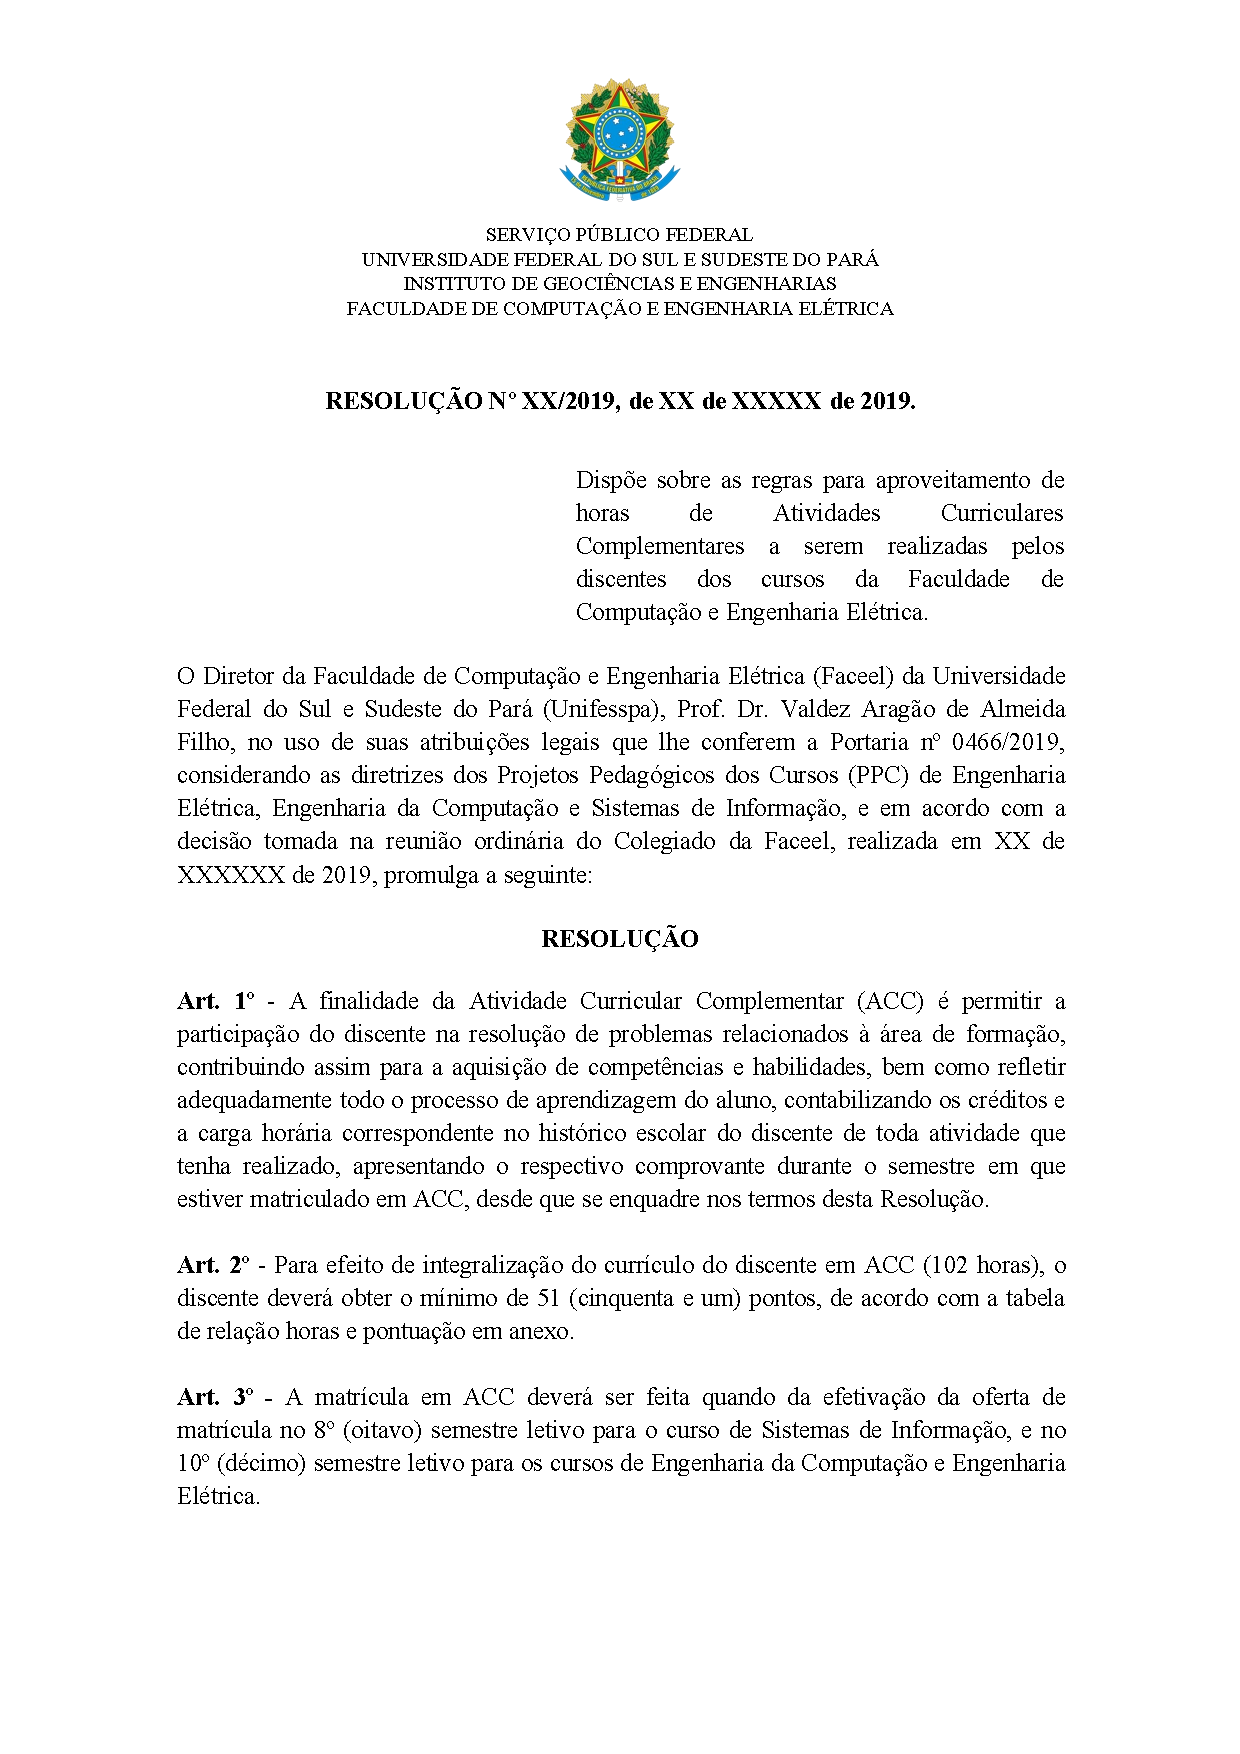
\includepdf[pages=-]{dados/anexos/regulamento_acc.pdf}

% Novo anexo-------------------------------------------------------------------
% \chapter{Nome do outro anexo}
% \label{chap:anexoB}

% conteúdo do outro anexo

\end{anexosenv}
 % Anexos

\end{document}
